This appendix presents the results of the closure tests used to validate the unfolding
procedures.  One hunded pseudoexperiments are constructed, each the weighted
number of events equal to the number of \emubb\ events observed in the data,
by varying the number of jets in the  baseline \ttbar\ +Wt simulation sample.
Each pseudoexperiment is unfolded and the bias ($N_{unfolded}-N_{true}$) and
pull ($(N_{unfolded}-N_{true})/\sigma_{unfolded}$) are calculated.  For each
bin in \pT\ and rank, the bias and pull distributions are fit to Gaussians.

%Figure~\ref{fig:UnfoldBias} shows the fitted mean of the bias for each bin in
\pT\ for jets of rank 1 through rank 5.  The shaded band indicates the fitted
sigma.  There is no evidence of statistically significant bias in the unfolding.

Figures~\ref{fig:appPull0} through~\ref{fig:appPull2} show the pull distributions 
for each bin, together with parameters of Gaussian fits to these distributions.
A summary of these results are also shown in Figure~\ref{fig:UnfoldPull}.  

% \begin{figure}

% 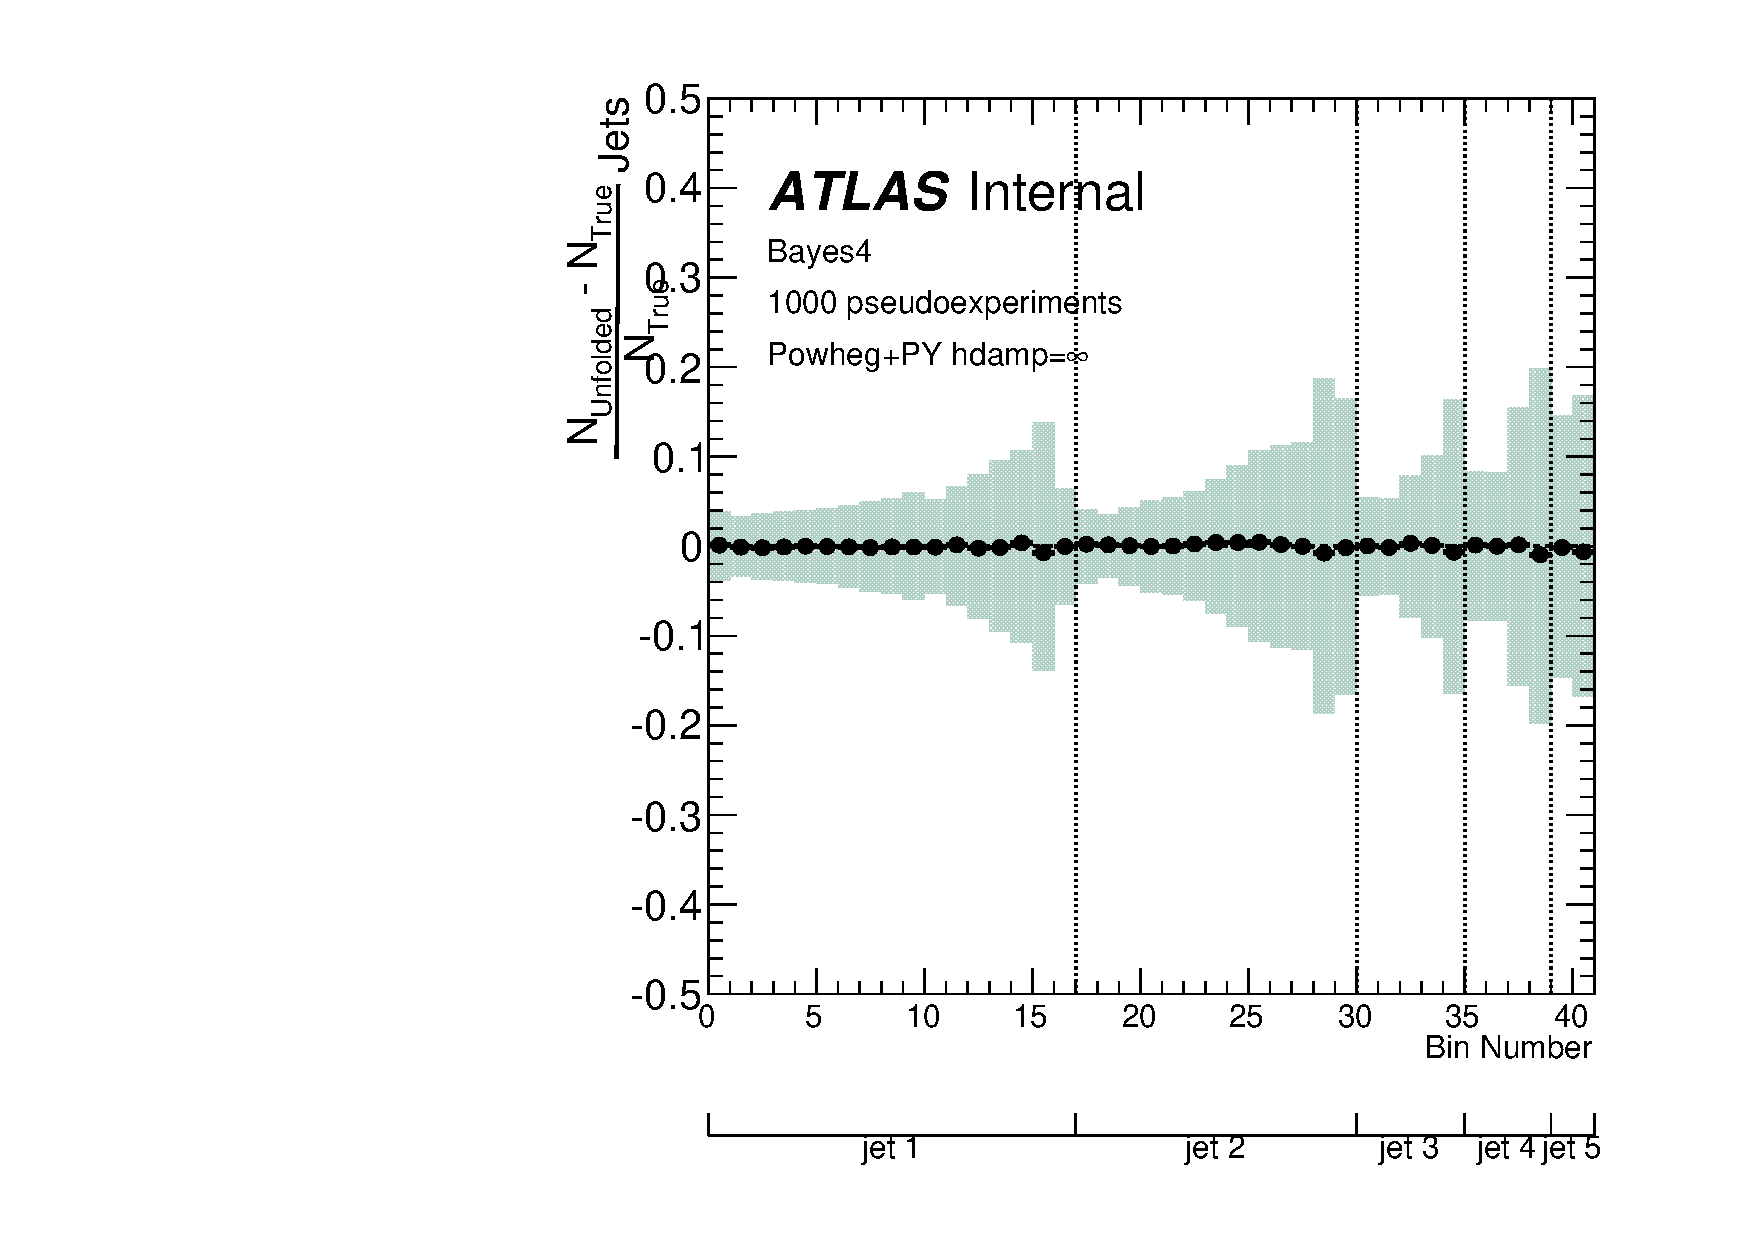
\includegraphics[width=0.9\textwidth]{fig/UnfoldPull/Bayes4Bias117050atlfast.pdf}

% \caption{Bias distributions for the extra jets from the baseline \ttbar\ +Wt simulation (\powpy) unfolded against a matrix filled with the baseline \ttbar\ +Wt simulation (\powpy). The Bayesian unfolding method 4 iterations is used. One thousand pseudoexperiments, each the size of the events in data, are randomly selected from the sample and unfolded.  A Gaussian is fit to the distributions of biases over the pseudoexperiments. The black points show the fitted mean of each bin. A fitted mean of zero shows the unfolding is not signifigantly biased. The blue band shows the fitted $\sigma$ of each bin.}
% \label{fig:UnfoldBias}
% \end{figure}
%\begin{subfigure}[]{0.5\textwidth}
\clearpage

\begin{figure}
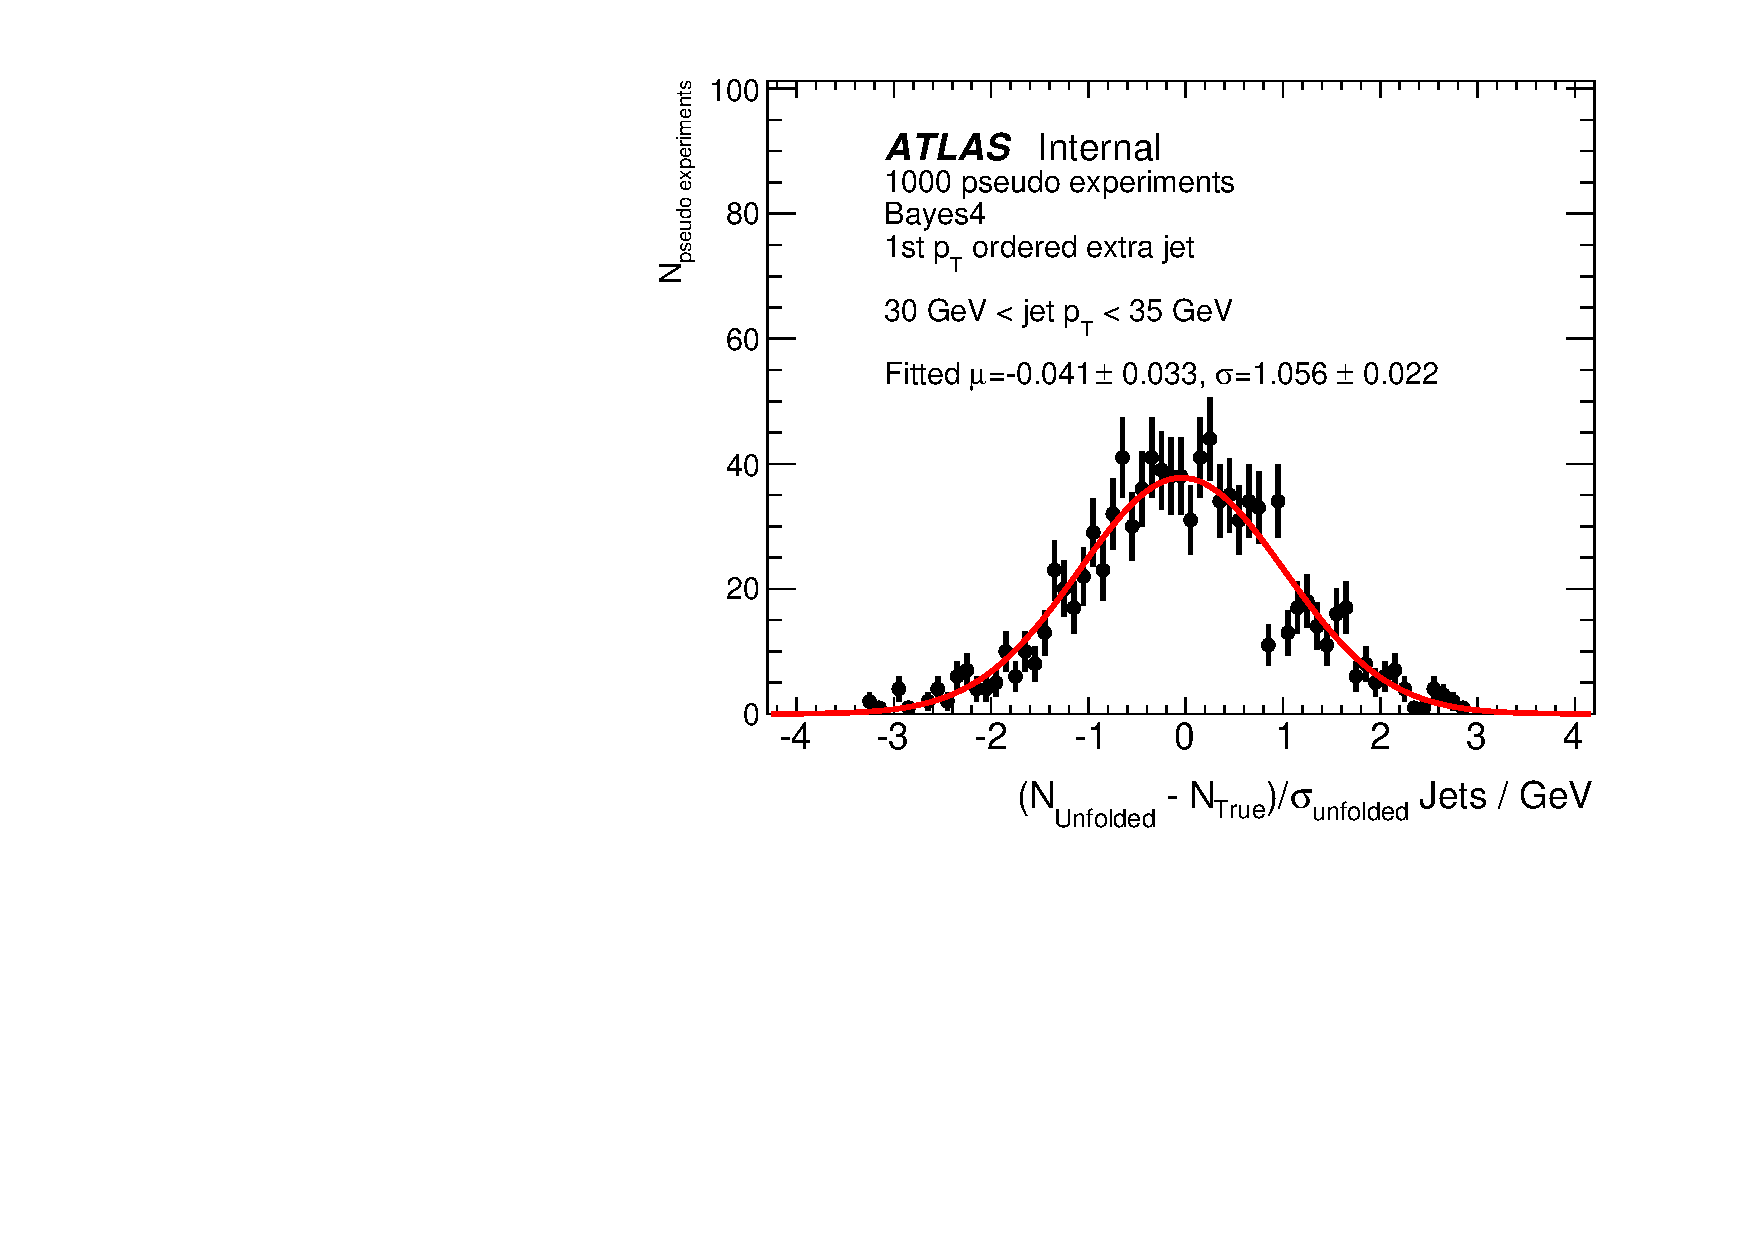
\includegraphics[width=0.33\textwidth]{fig/UnfoldPull/SingleSlicePull1.pdf}
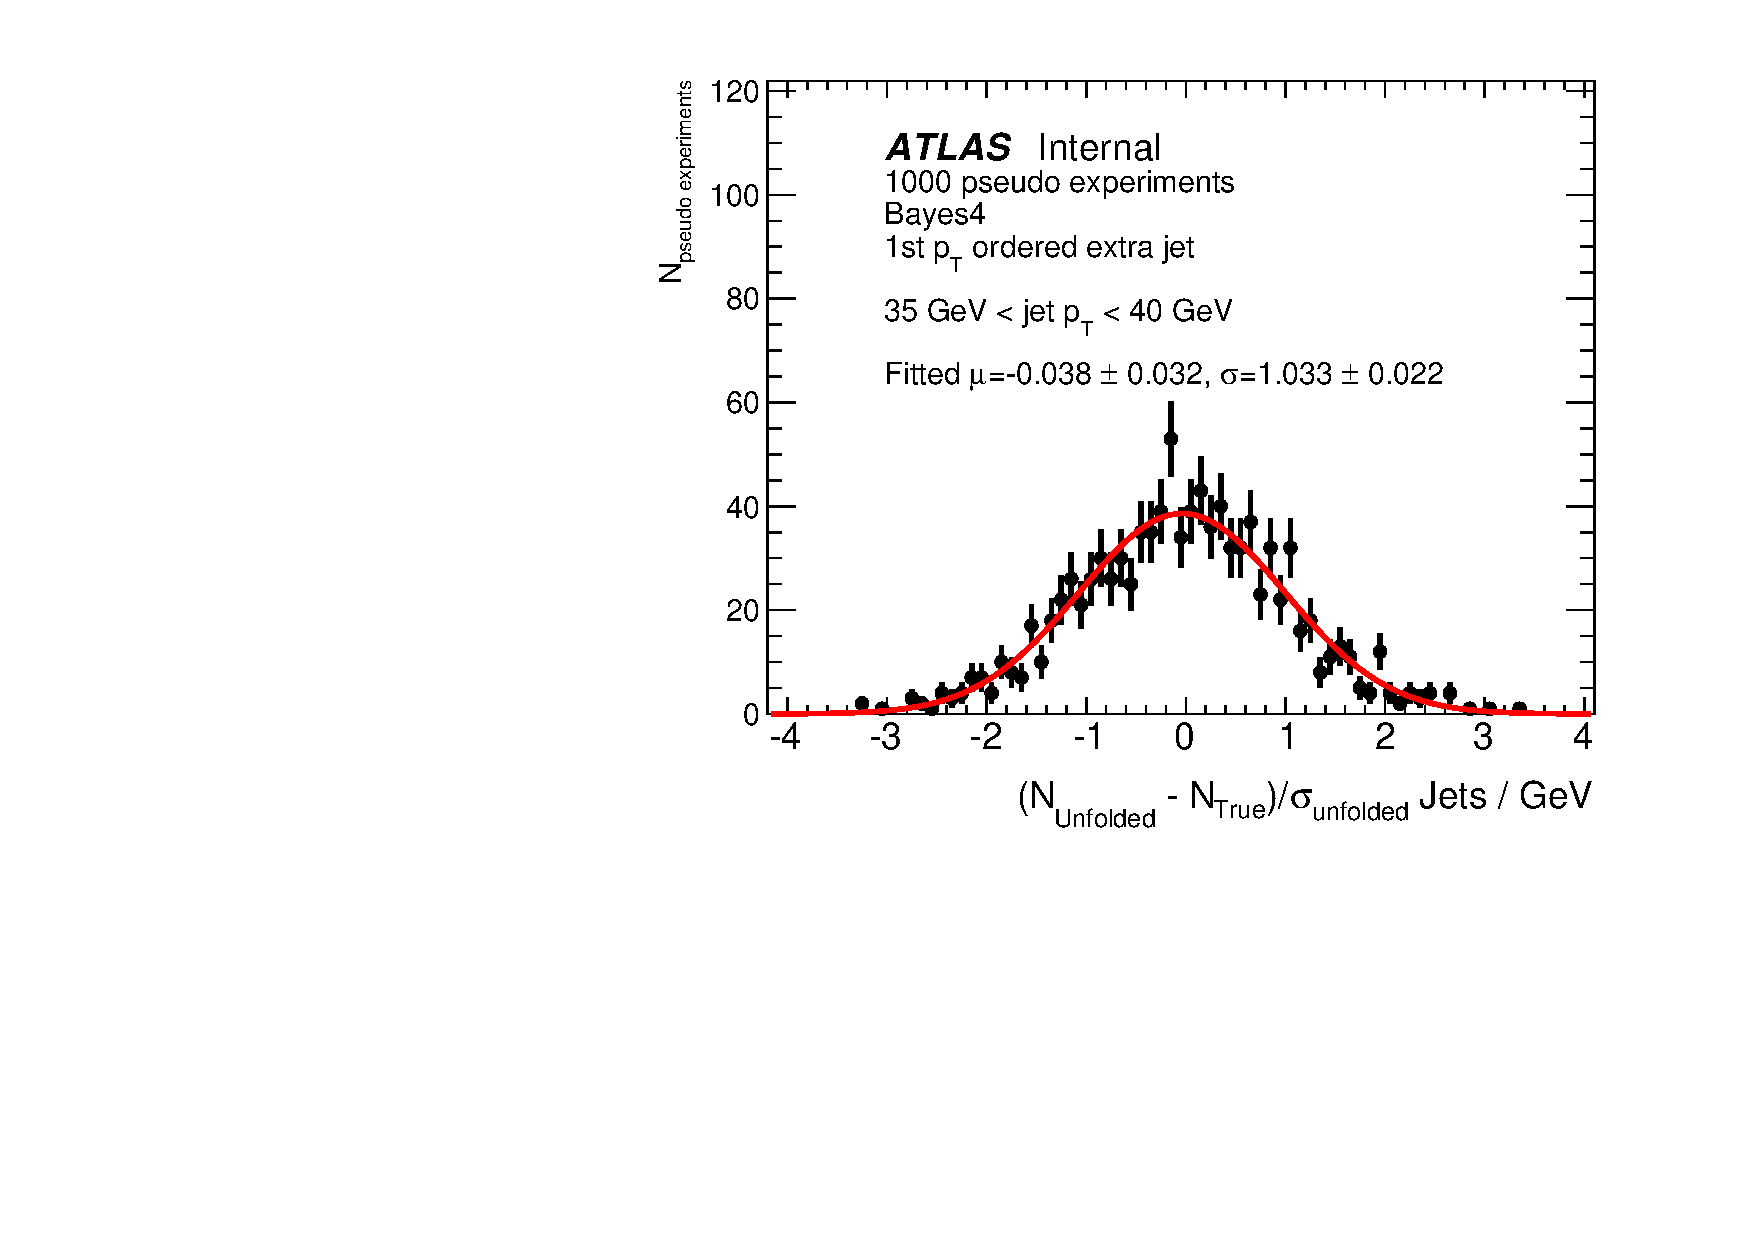
\includegraphics[width=0.33\textwidth]{fig/UnfoldPull/SingleSlicePull2.pdf}
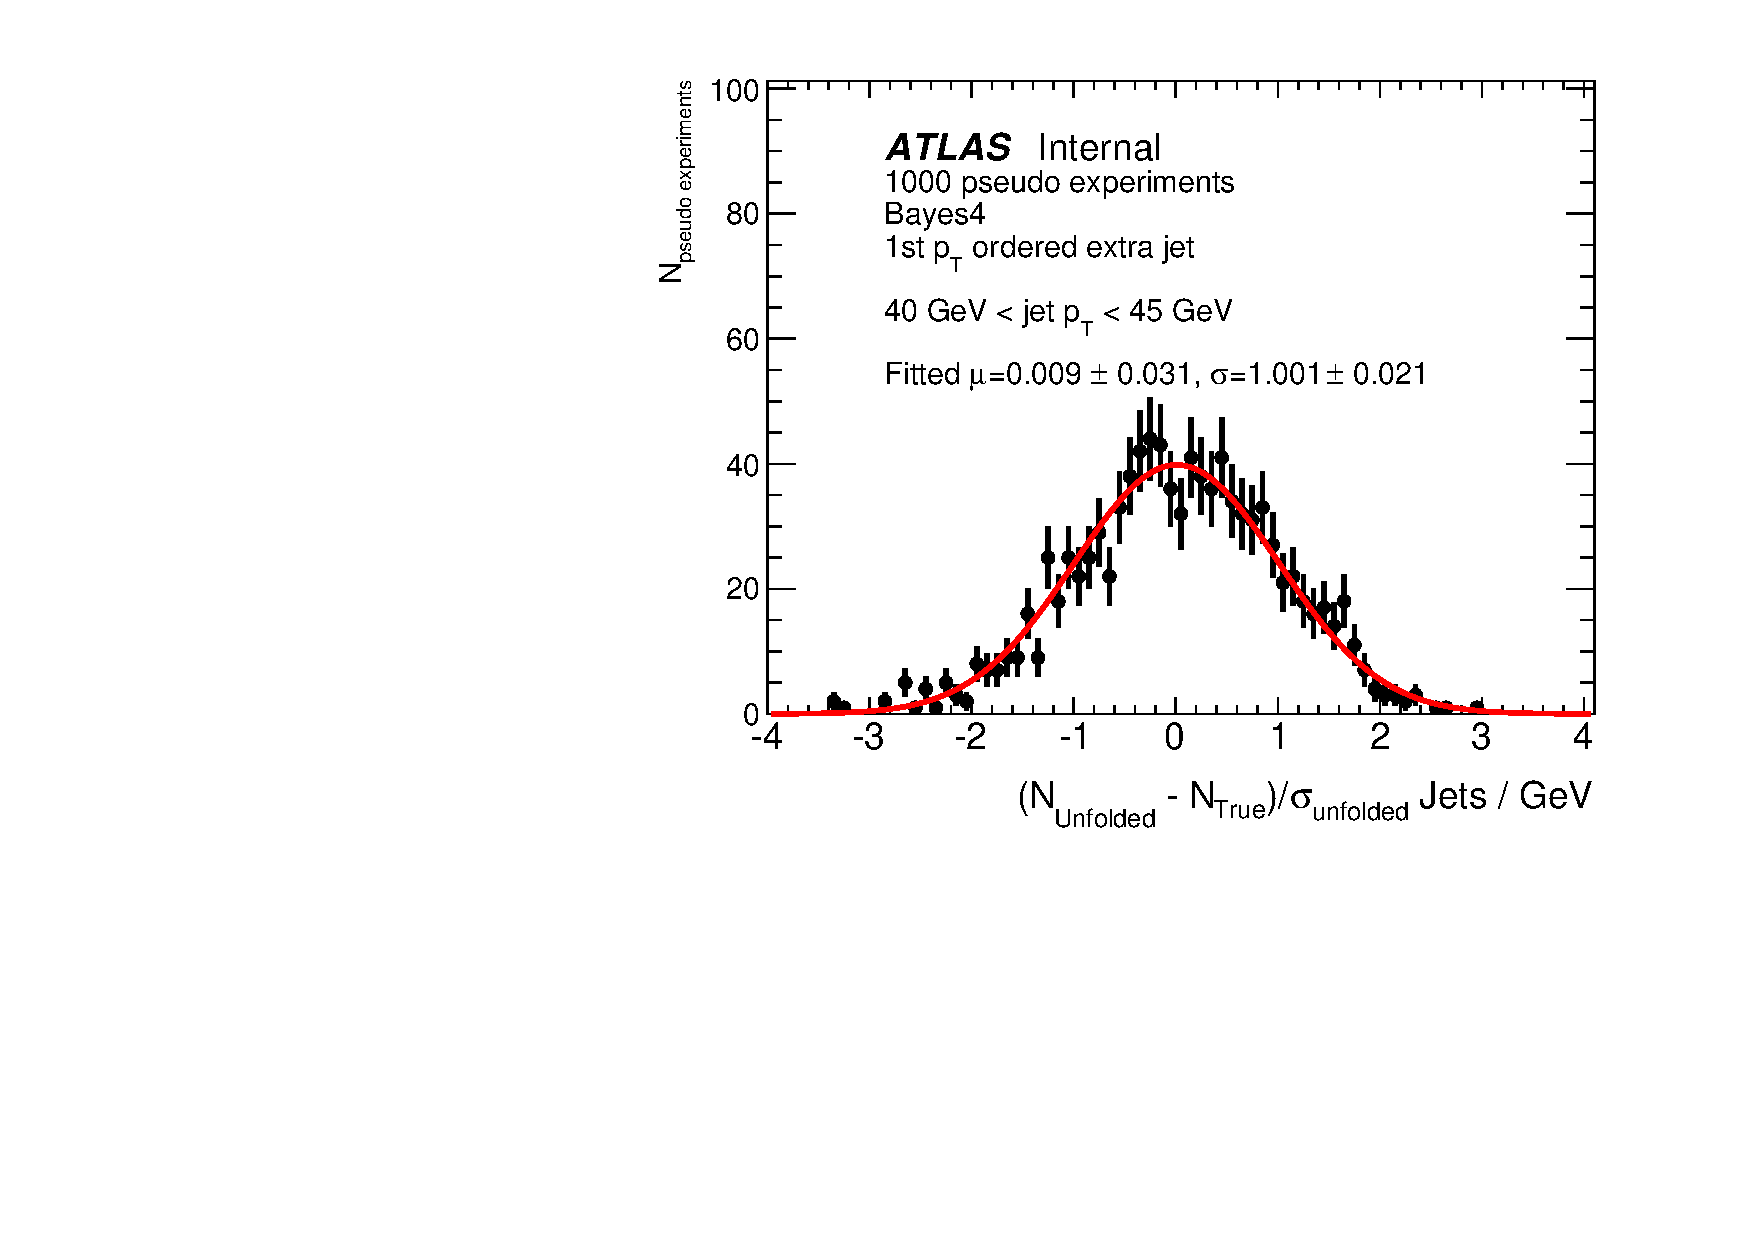
\includegraphics[width=0.33\textwidth]{fig/UnfoldPull/SingleSlicePull3.pdf}
%
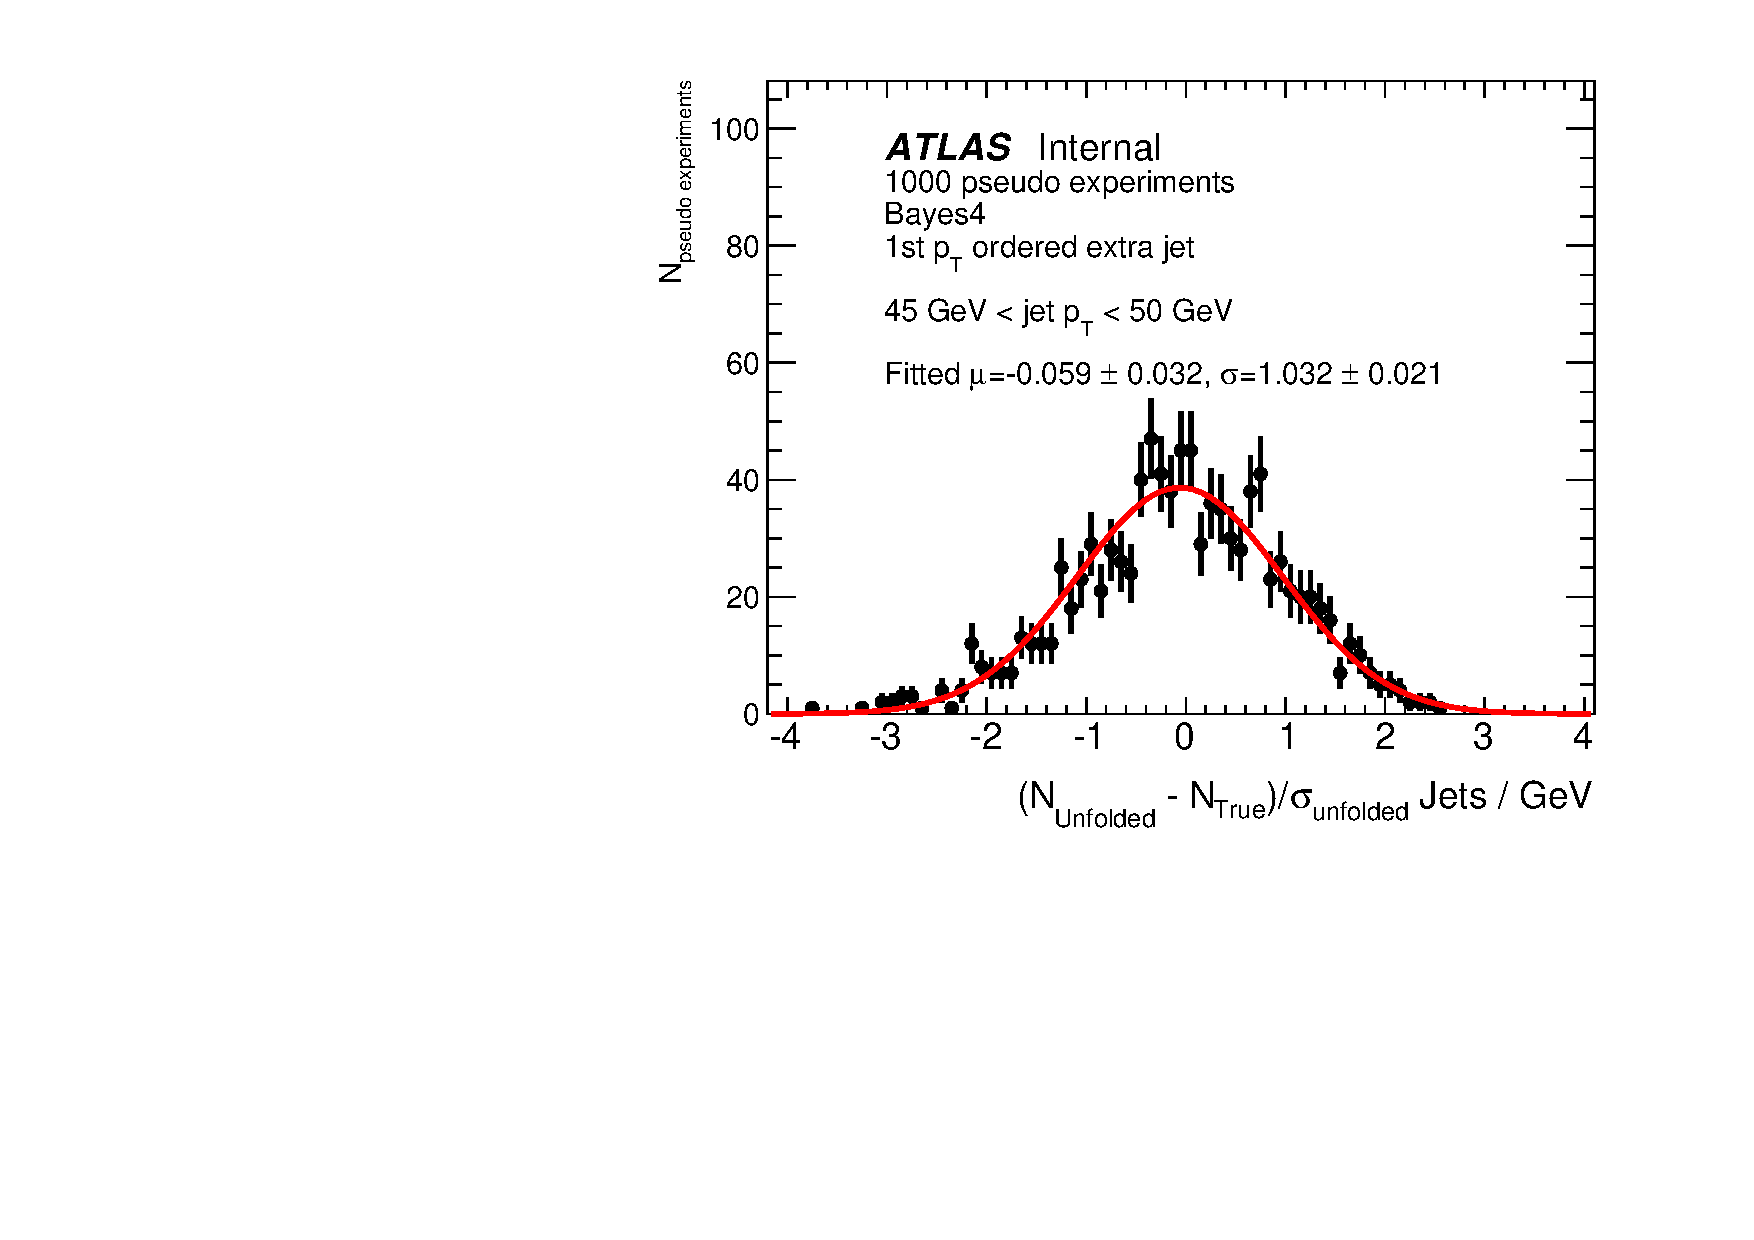
\includegraphics[width=0.33\textwidth]{fig/UnfoldPull/SingleSlicePull4.pdf}
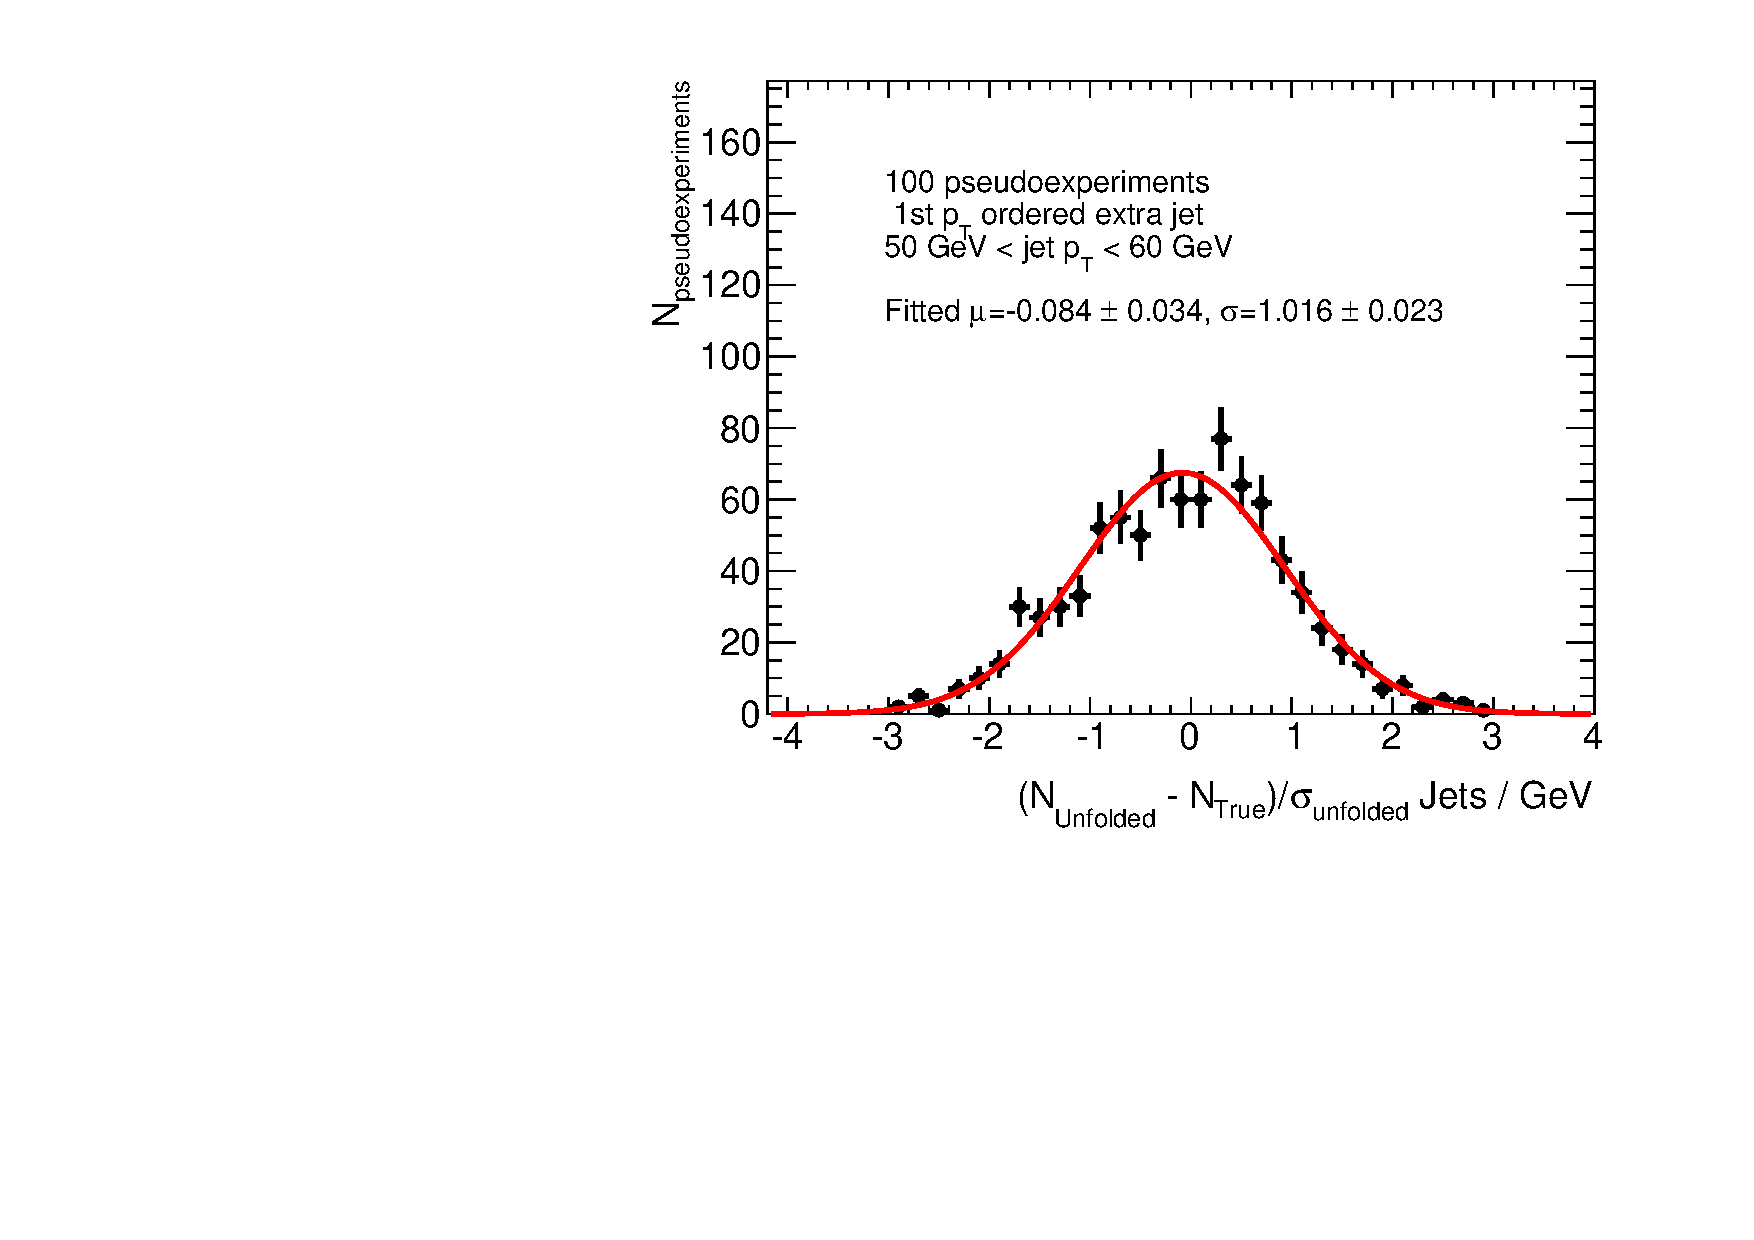
\includegraphics[width=0.33\textwidth]{fig/UnfoldPull/SingleSlicePull5.pdf}
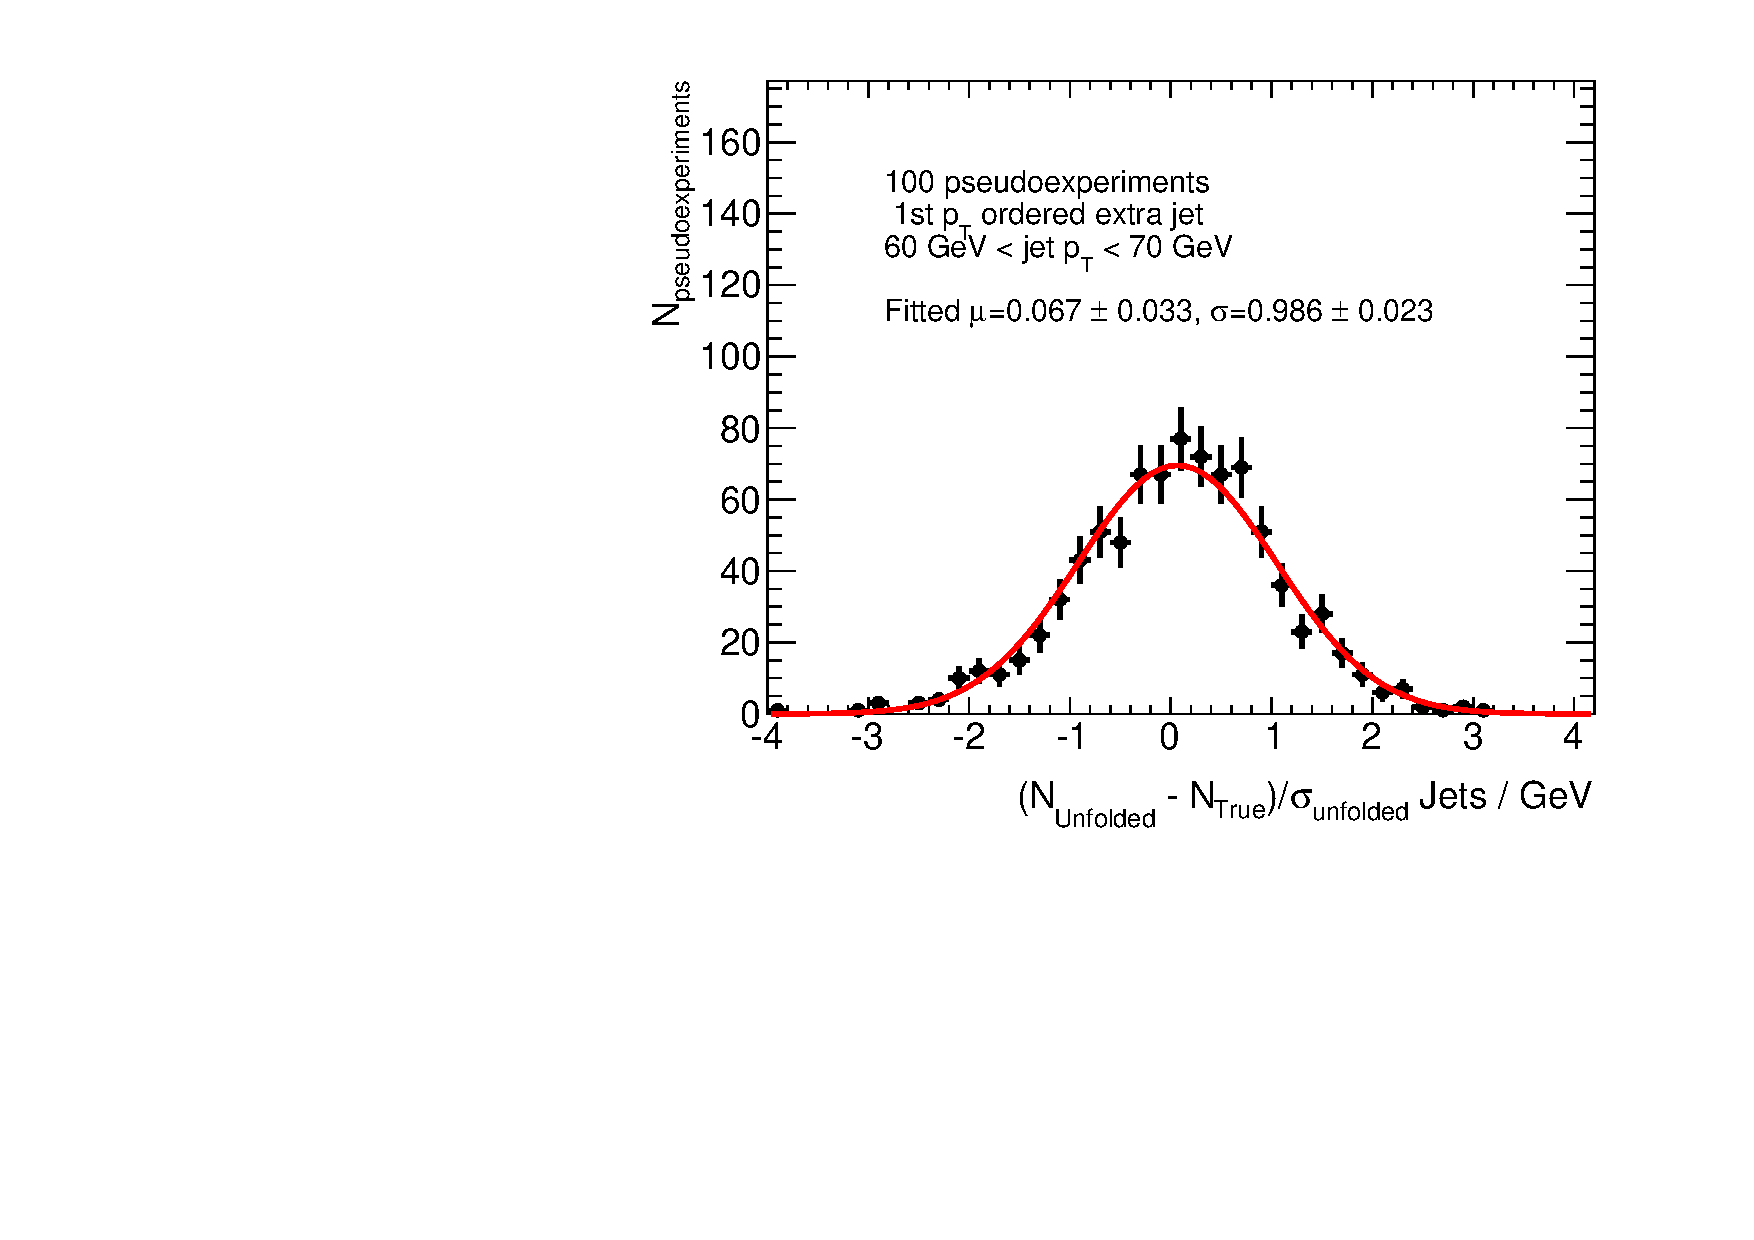
\includegraphics[width=0.33\textwidth]{fig/UnfoldPull/SingleSlicePull6.pdf}
%
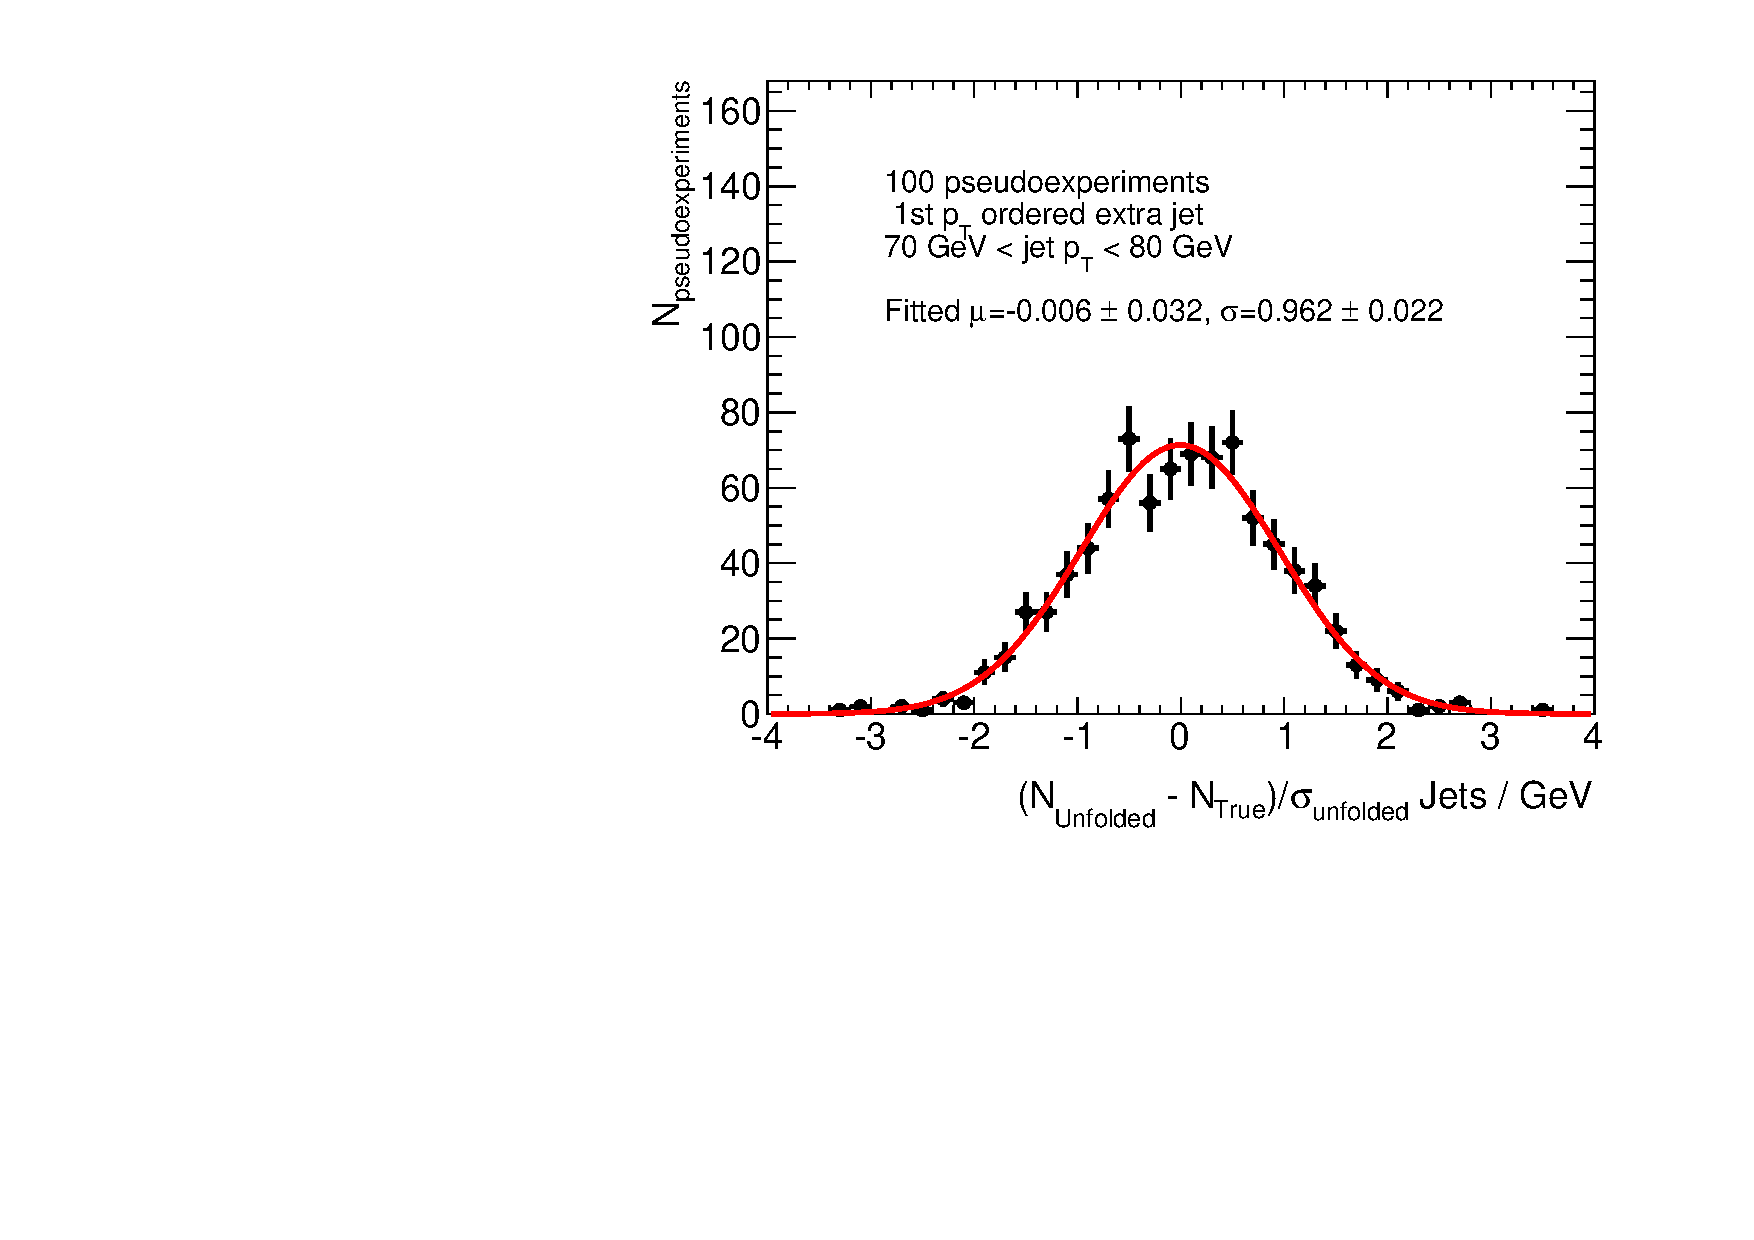
\includegraphics[width=0.33\textwidth]{fig/UnfoldPull/SingleSlicePull7.pdf}
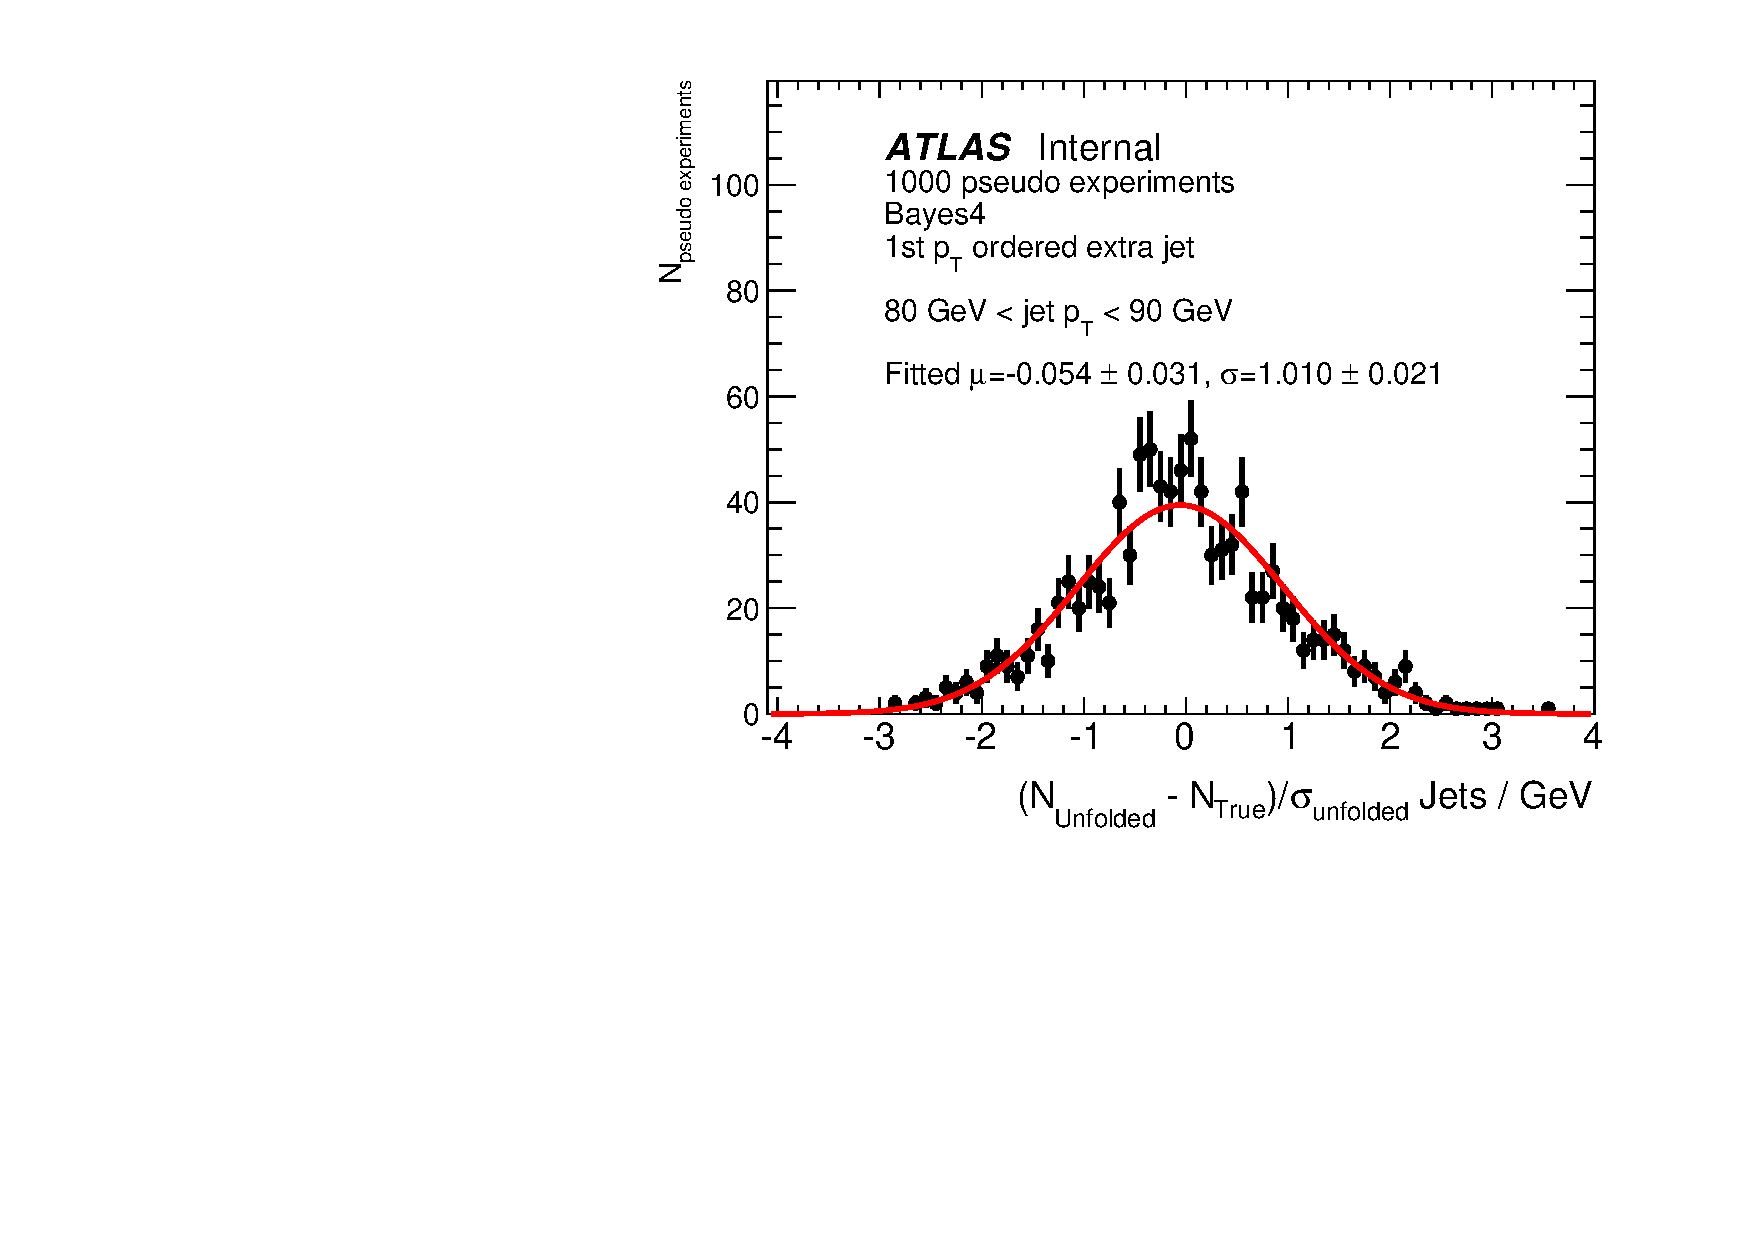
\includegraphics[width=0.33\textwidth]{fig/UnfoldPull/SingleSlicePull8.pdf}
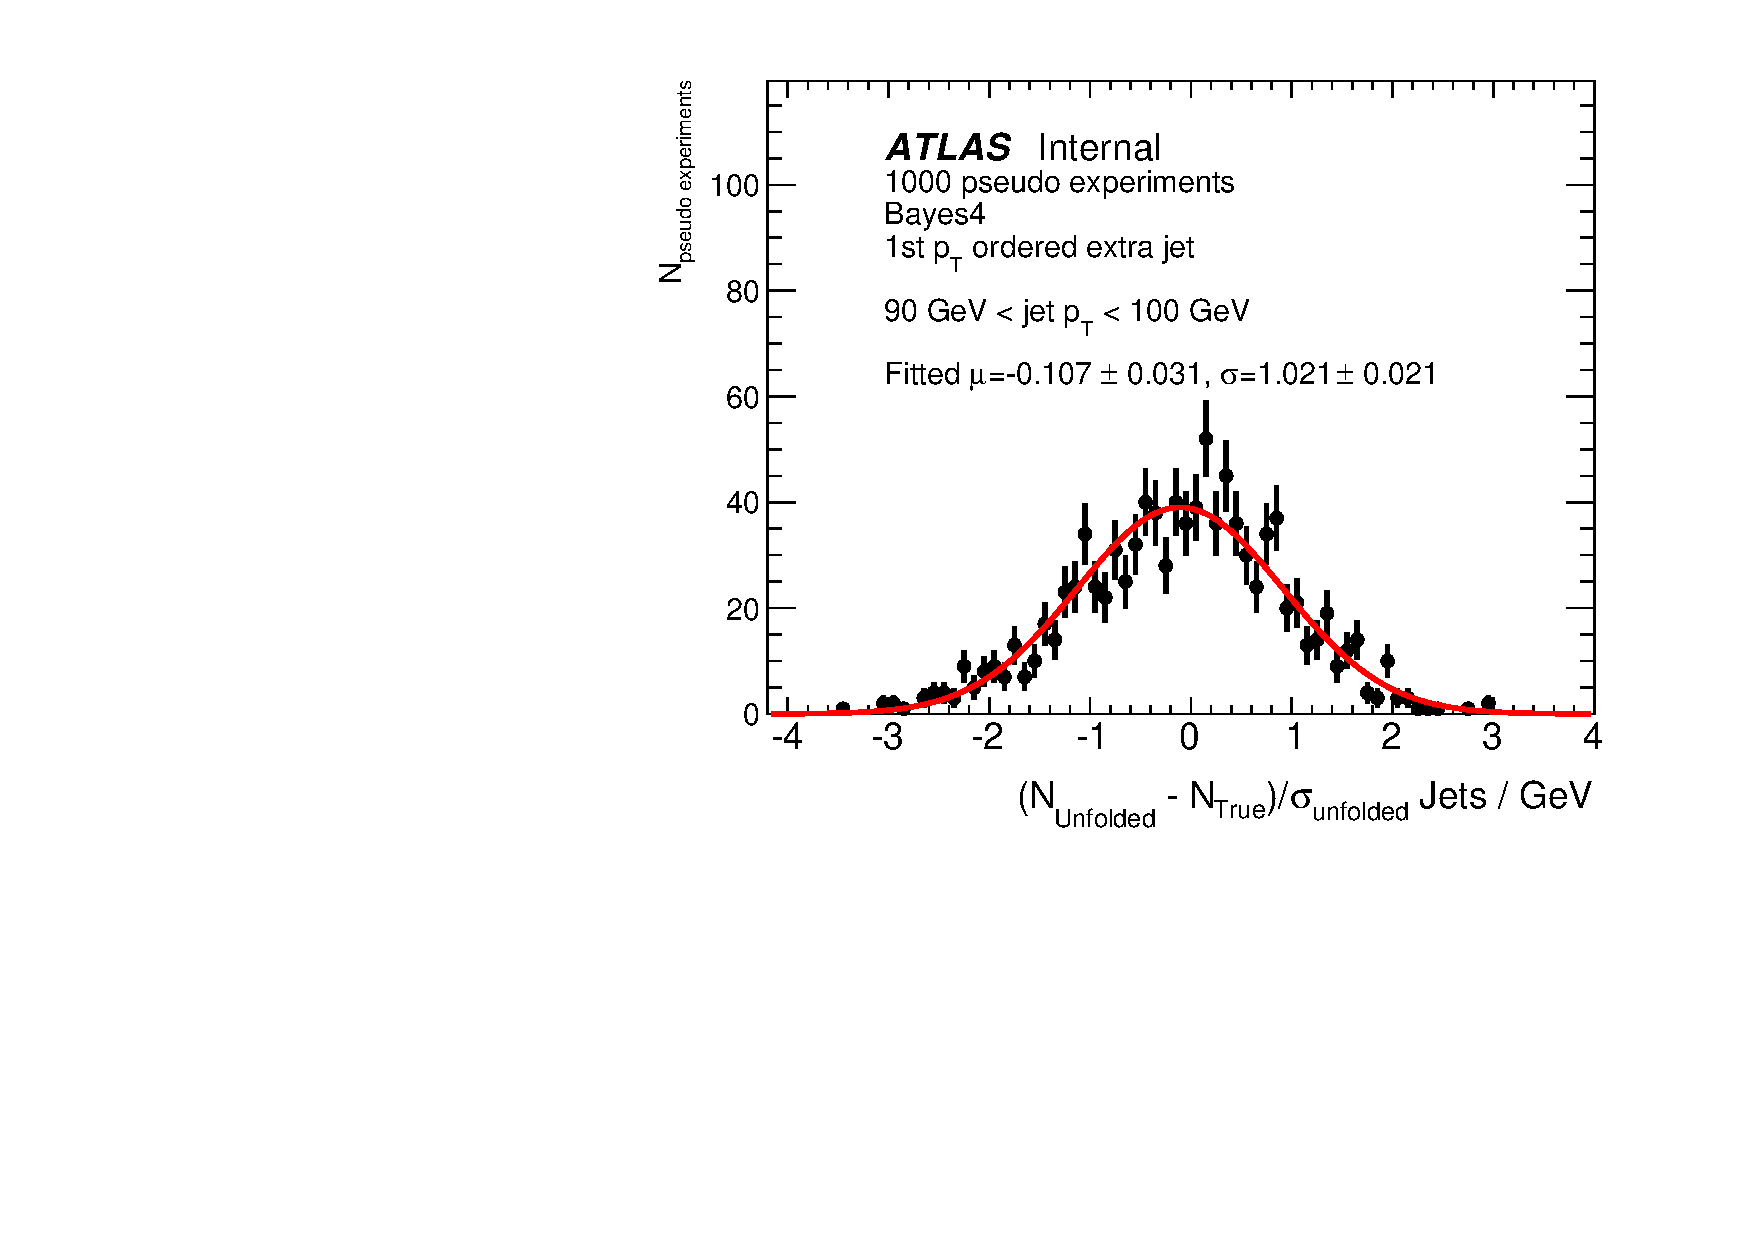
\includegraphics[width=0.33\textwidth]{fig/UnfoldPull/SingleSlicePull9.pdf}
%
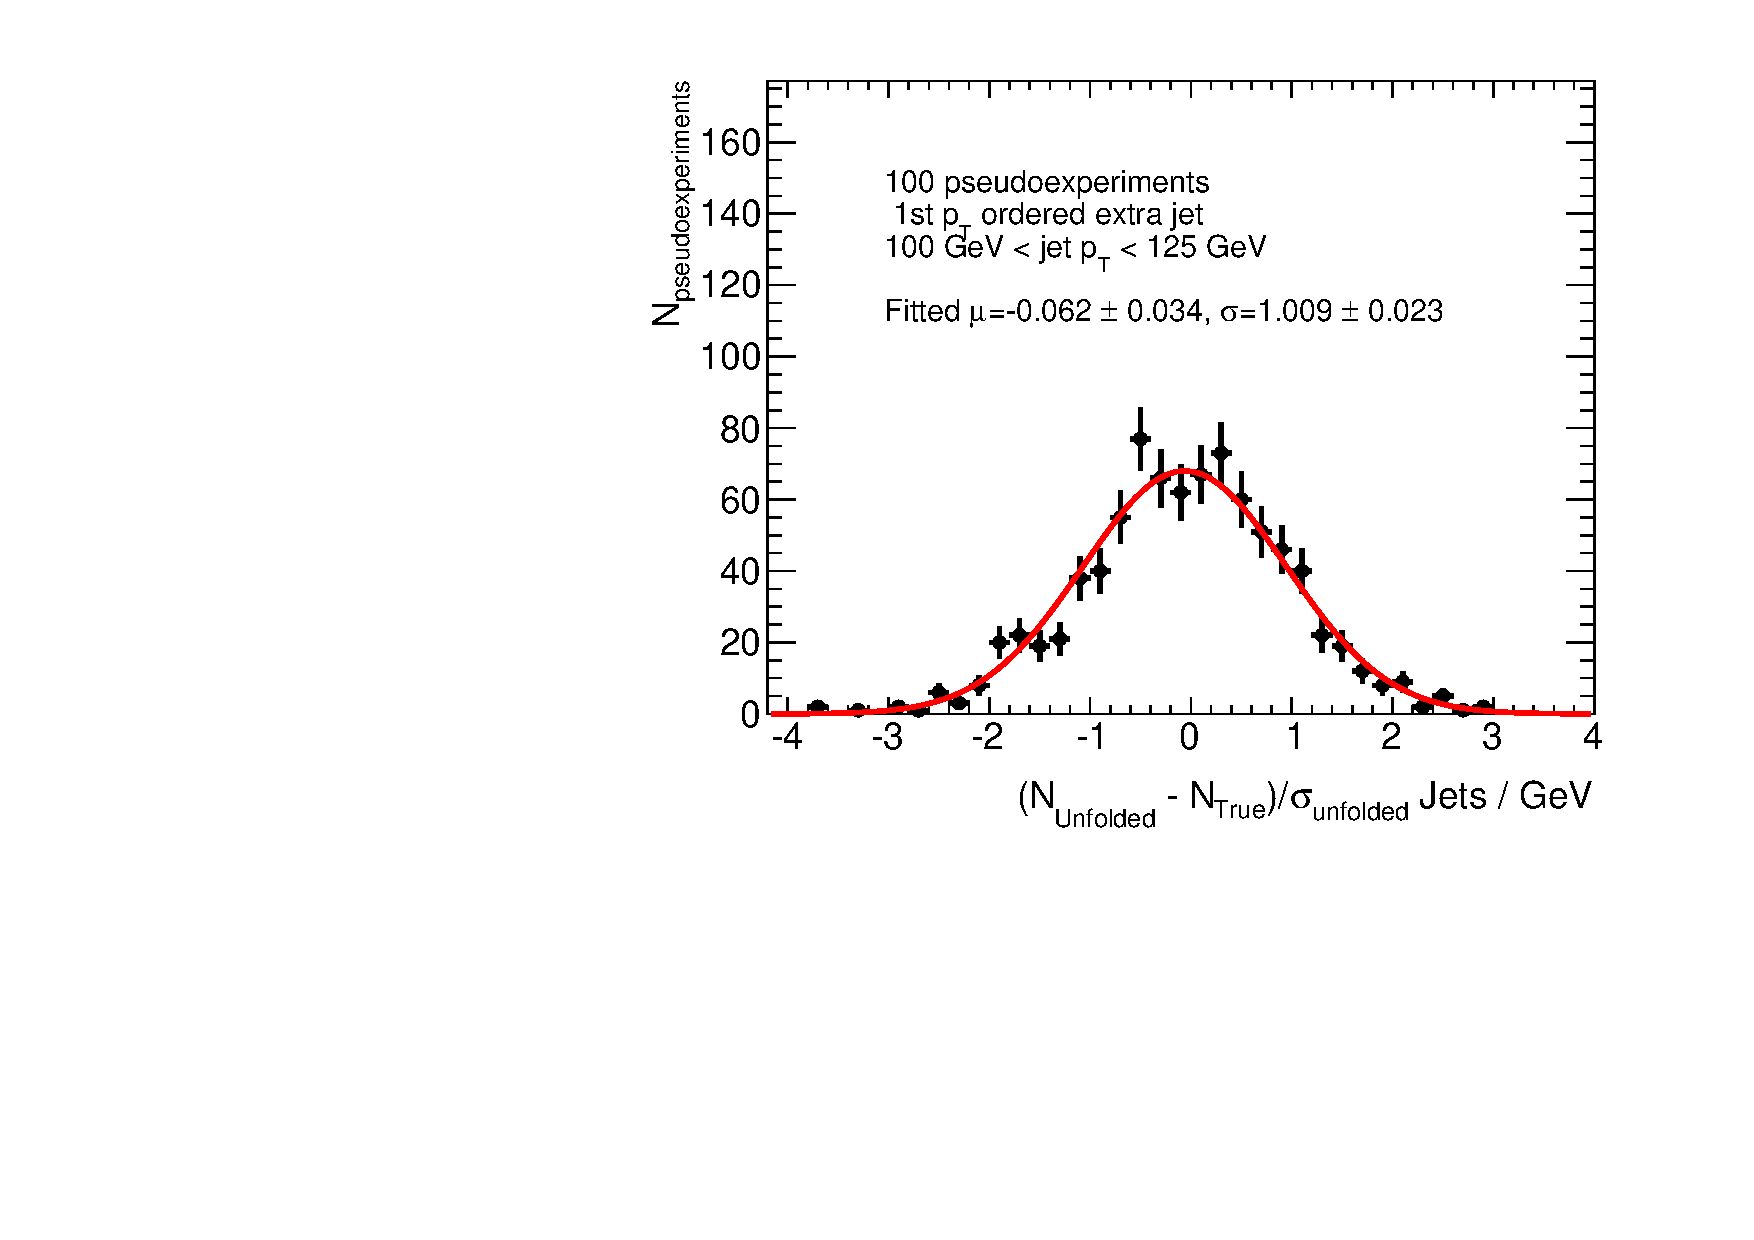
\includegraphics[width=0.33\textwidth]{fig/UnfoldPull/SingleSlicePull10.pdf}
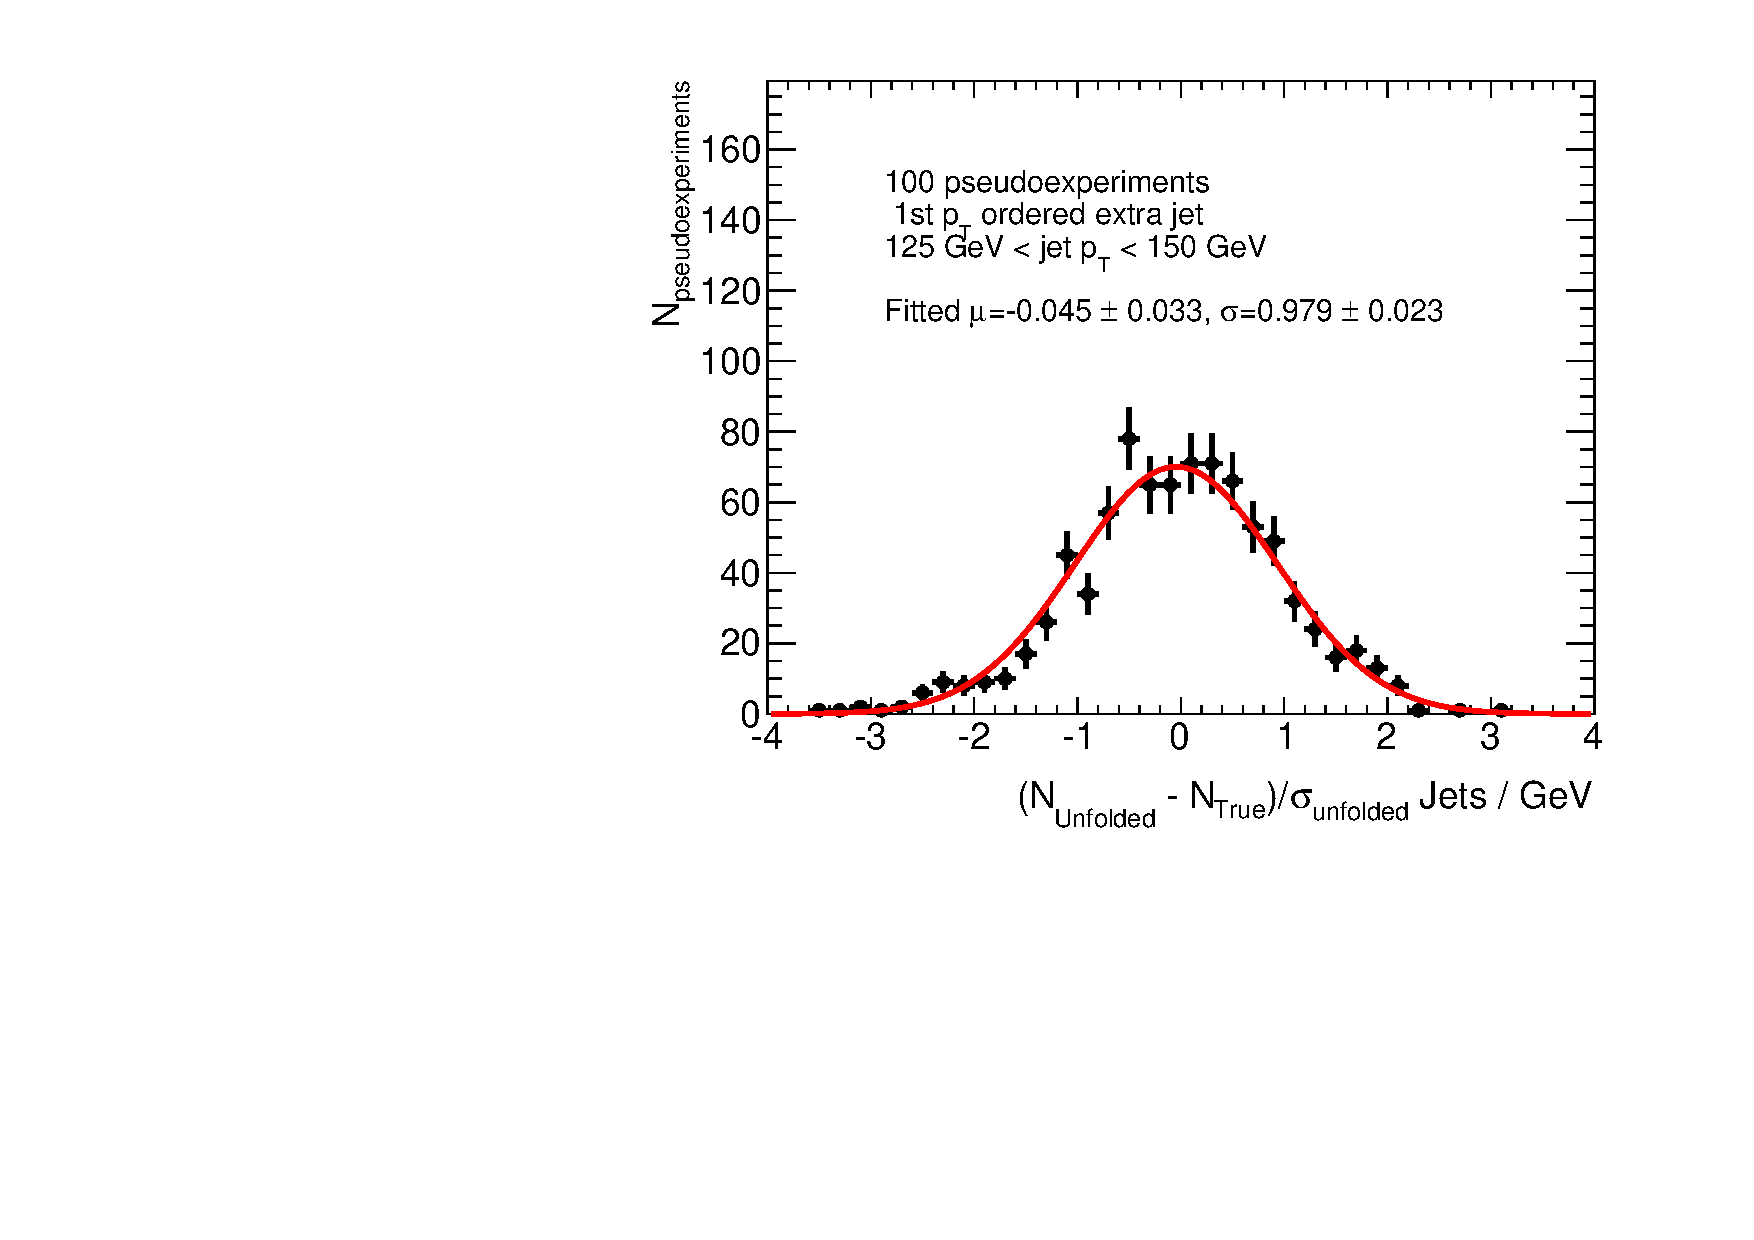
\includegraphics[width=0.33\textwidth]{fig/UnfoldPull/SingleSlicePull11.pdf}
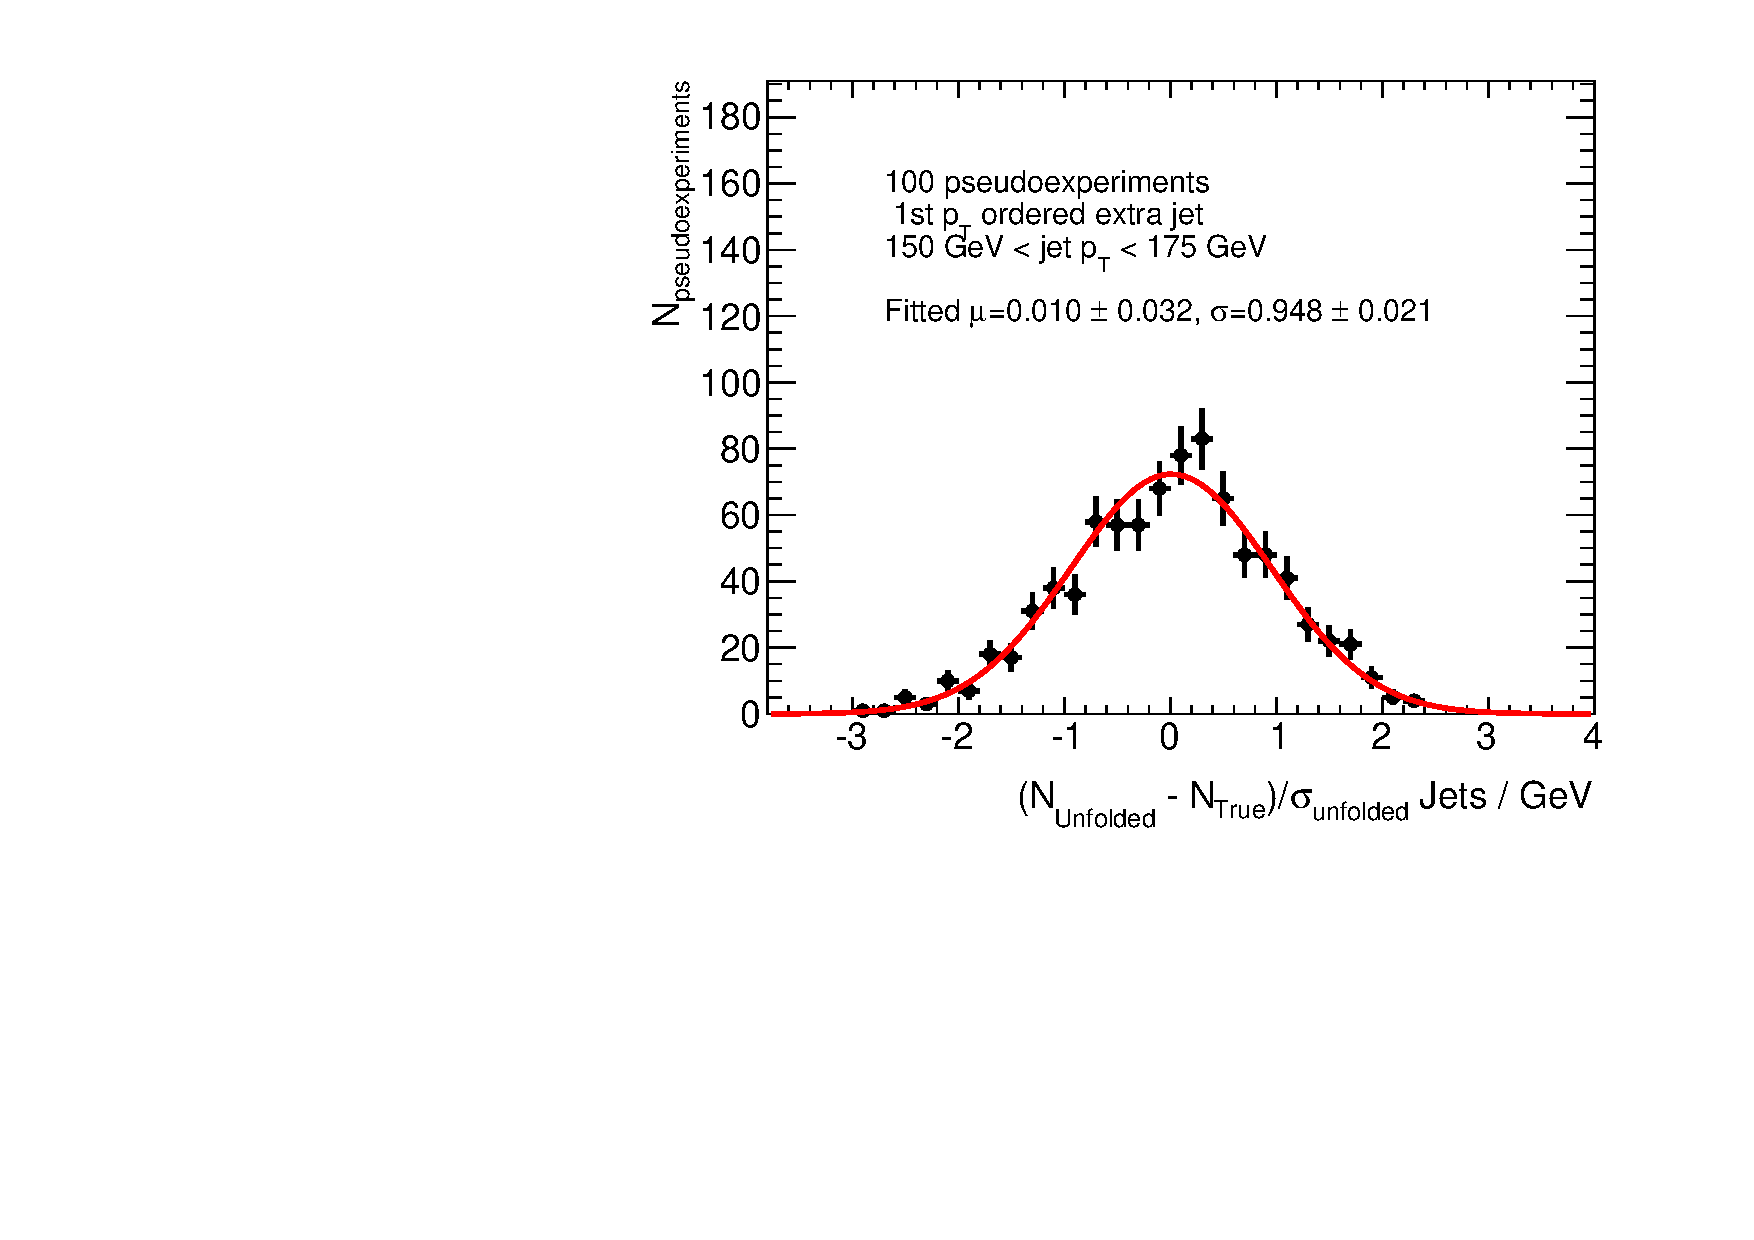
\includegraphics[width=0.33\textwidth]{fig/UnfoldPull/SingleSlicePull12.pdf}
%
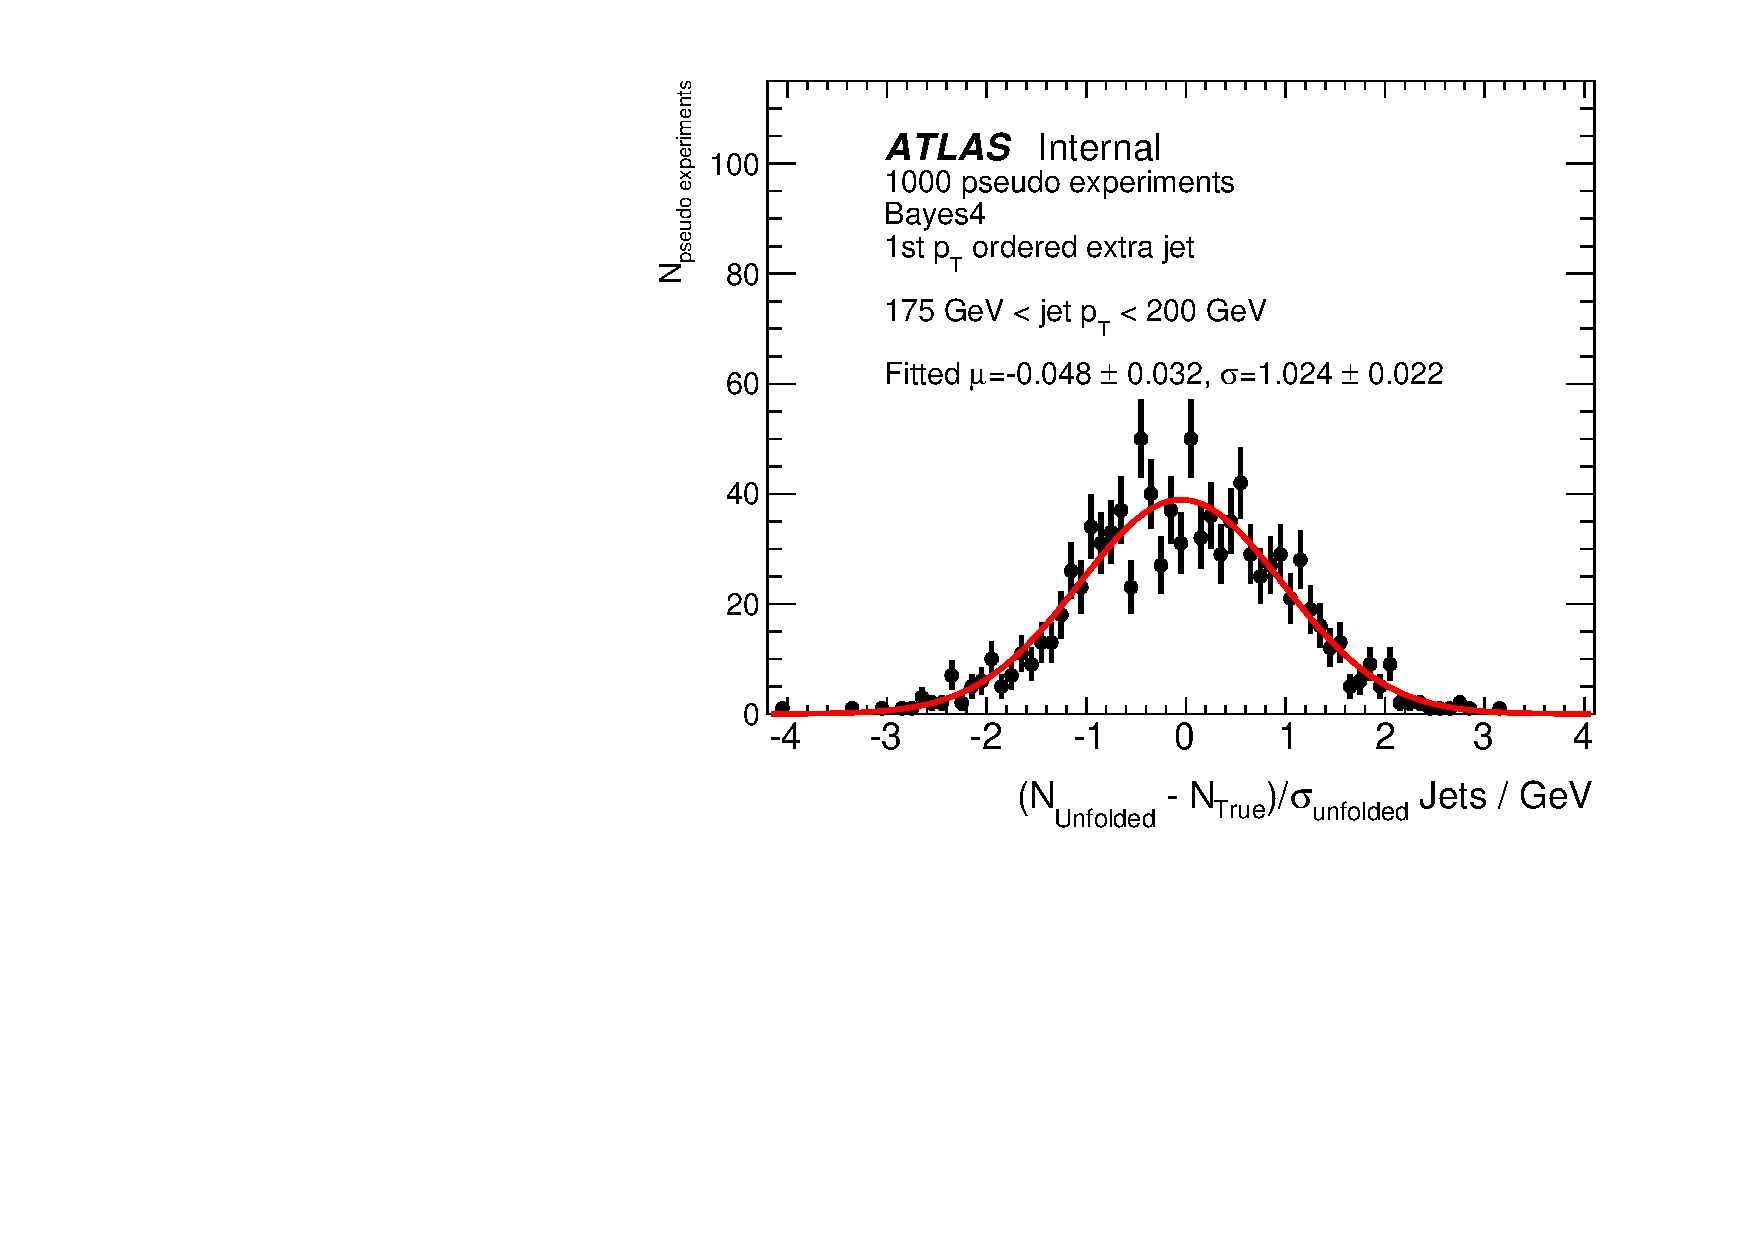
\includegraphics[width=0.33\textwidth]{fig/UnfoldPull/SingleSlicePull13.pdf}
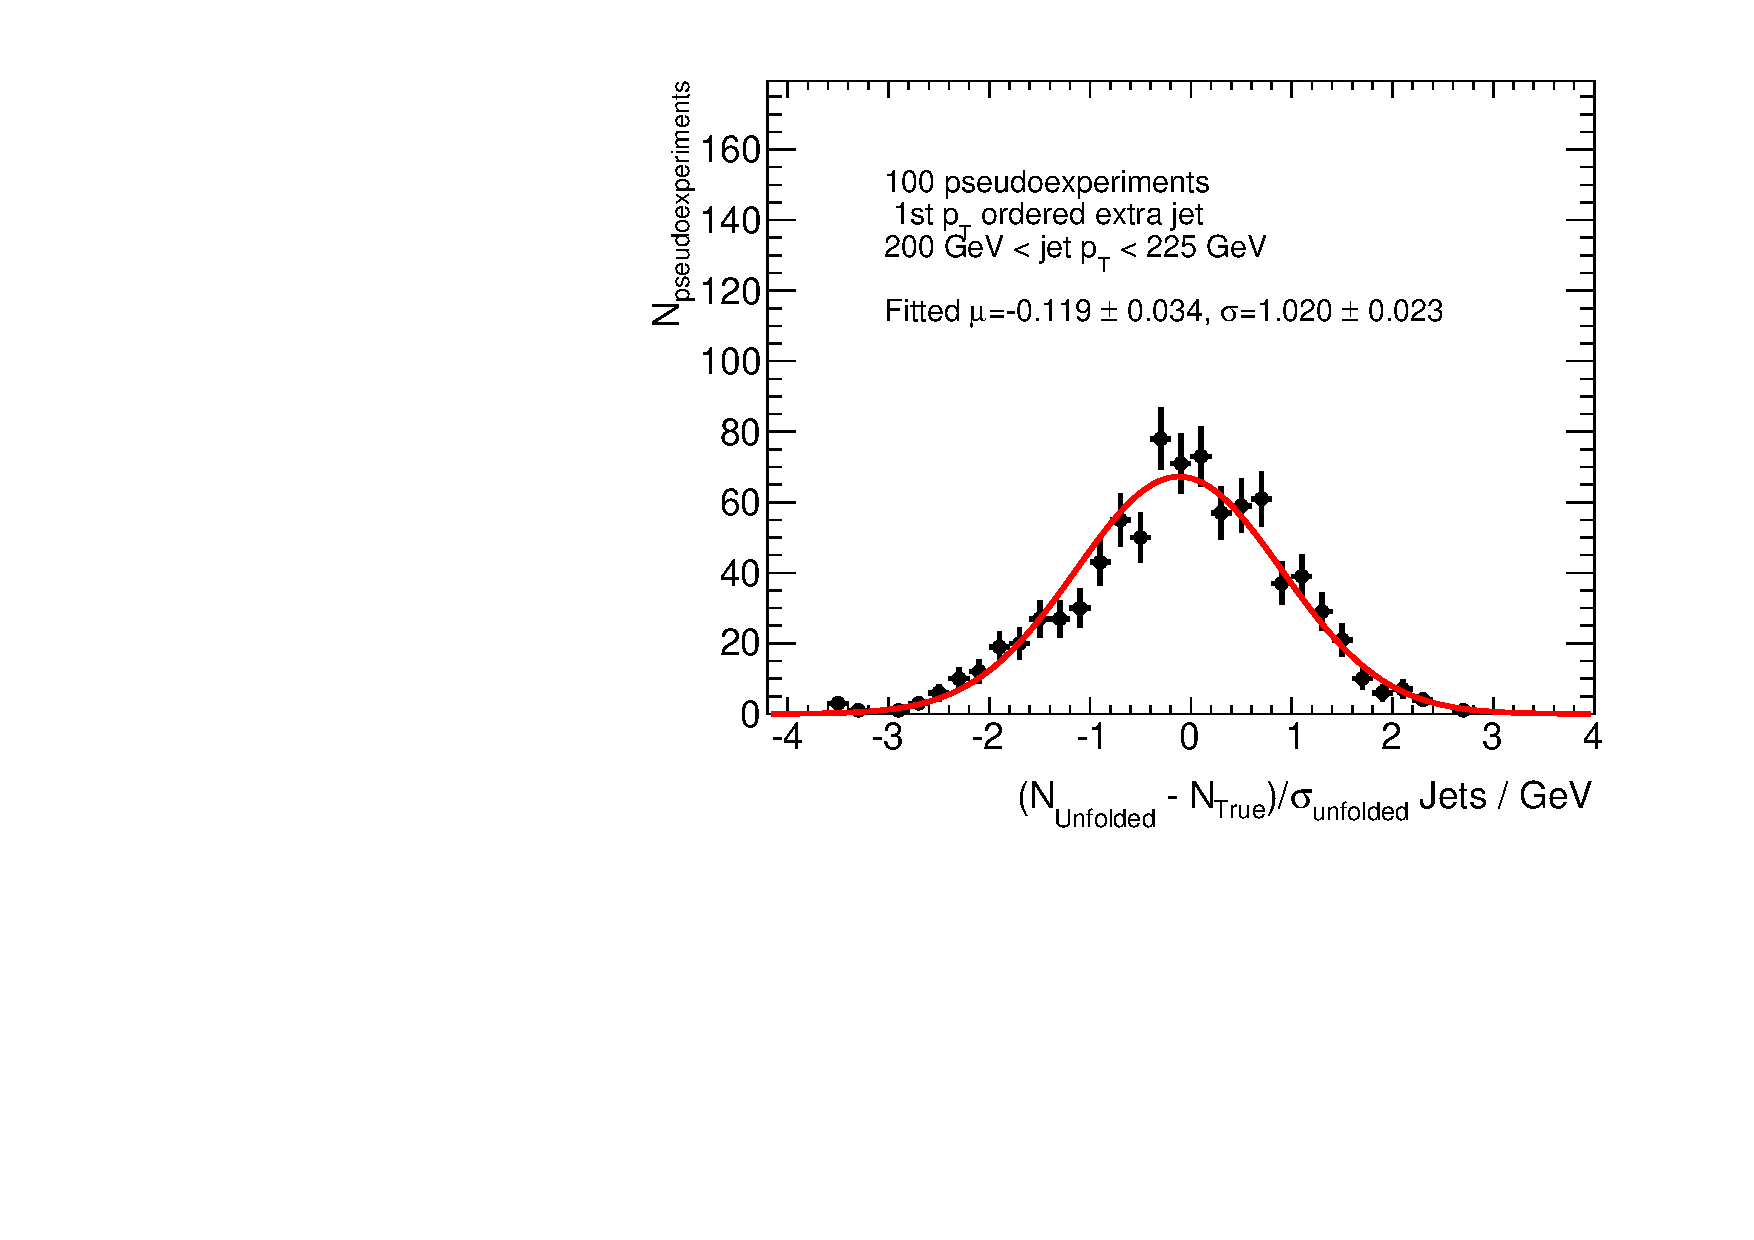
\includegraphics[width=0.33\textwidth]{fig/UnfoldPull/SingleSlicePull14.pdf}
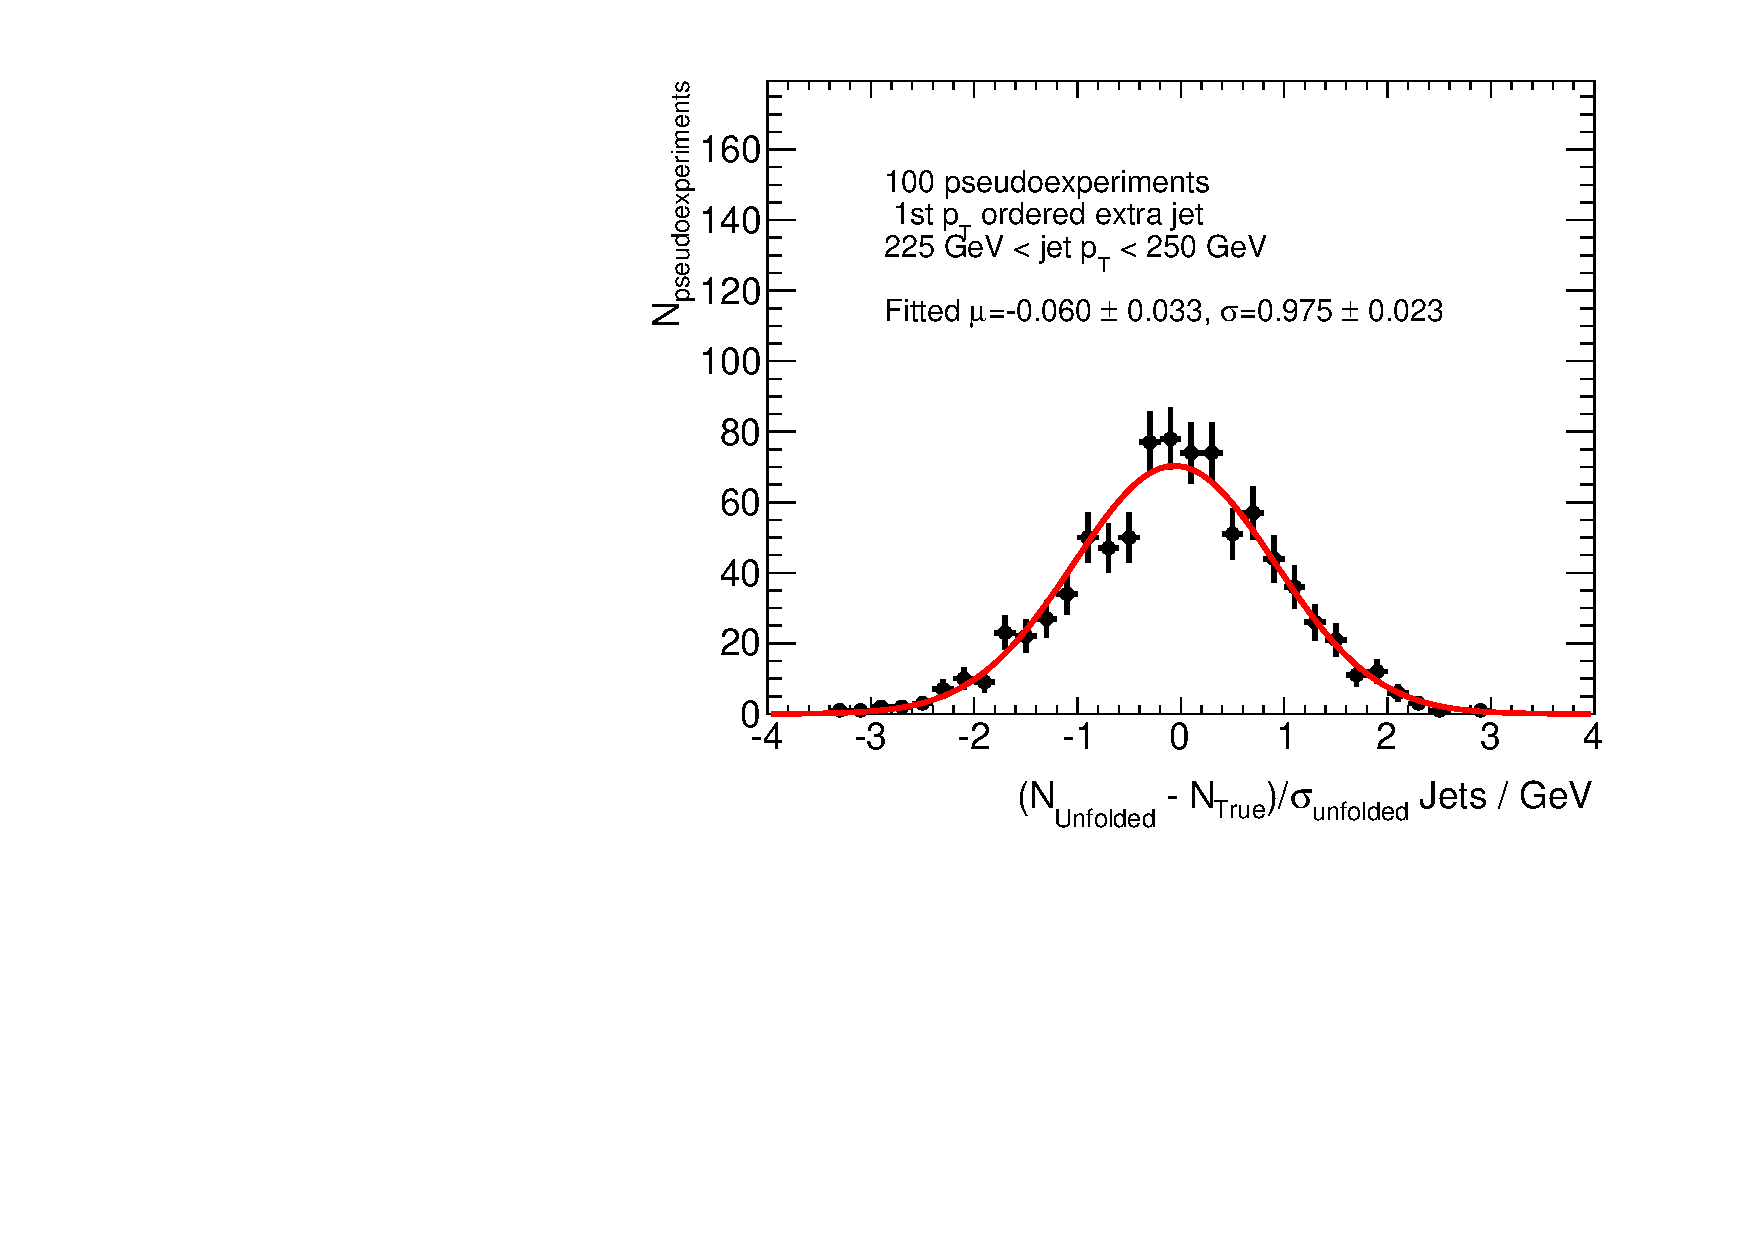
\includegraphics[width=0.33\textwidth]{fig/UnfoldPull/SingleSlicePull15.pdf}
\caption{Pull distributions for the extra jets from the baseline \ttbar\ +Wt simulation (\powpy) unfolded against a matrix filled with the baseline \ttbar\ +Wt simulation (\powpy). The Bayesian unfolding method 4 iterations is used. One thousand pseudoexperiments, each the size of the events in data, are randomly selected from the sample and unfolded.  A Gaussian is fit to the distributions of biases over the pseudoexperiments}
\label{fig:appPull0}
\end{figure}
\begin{figure}
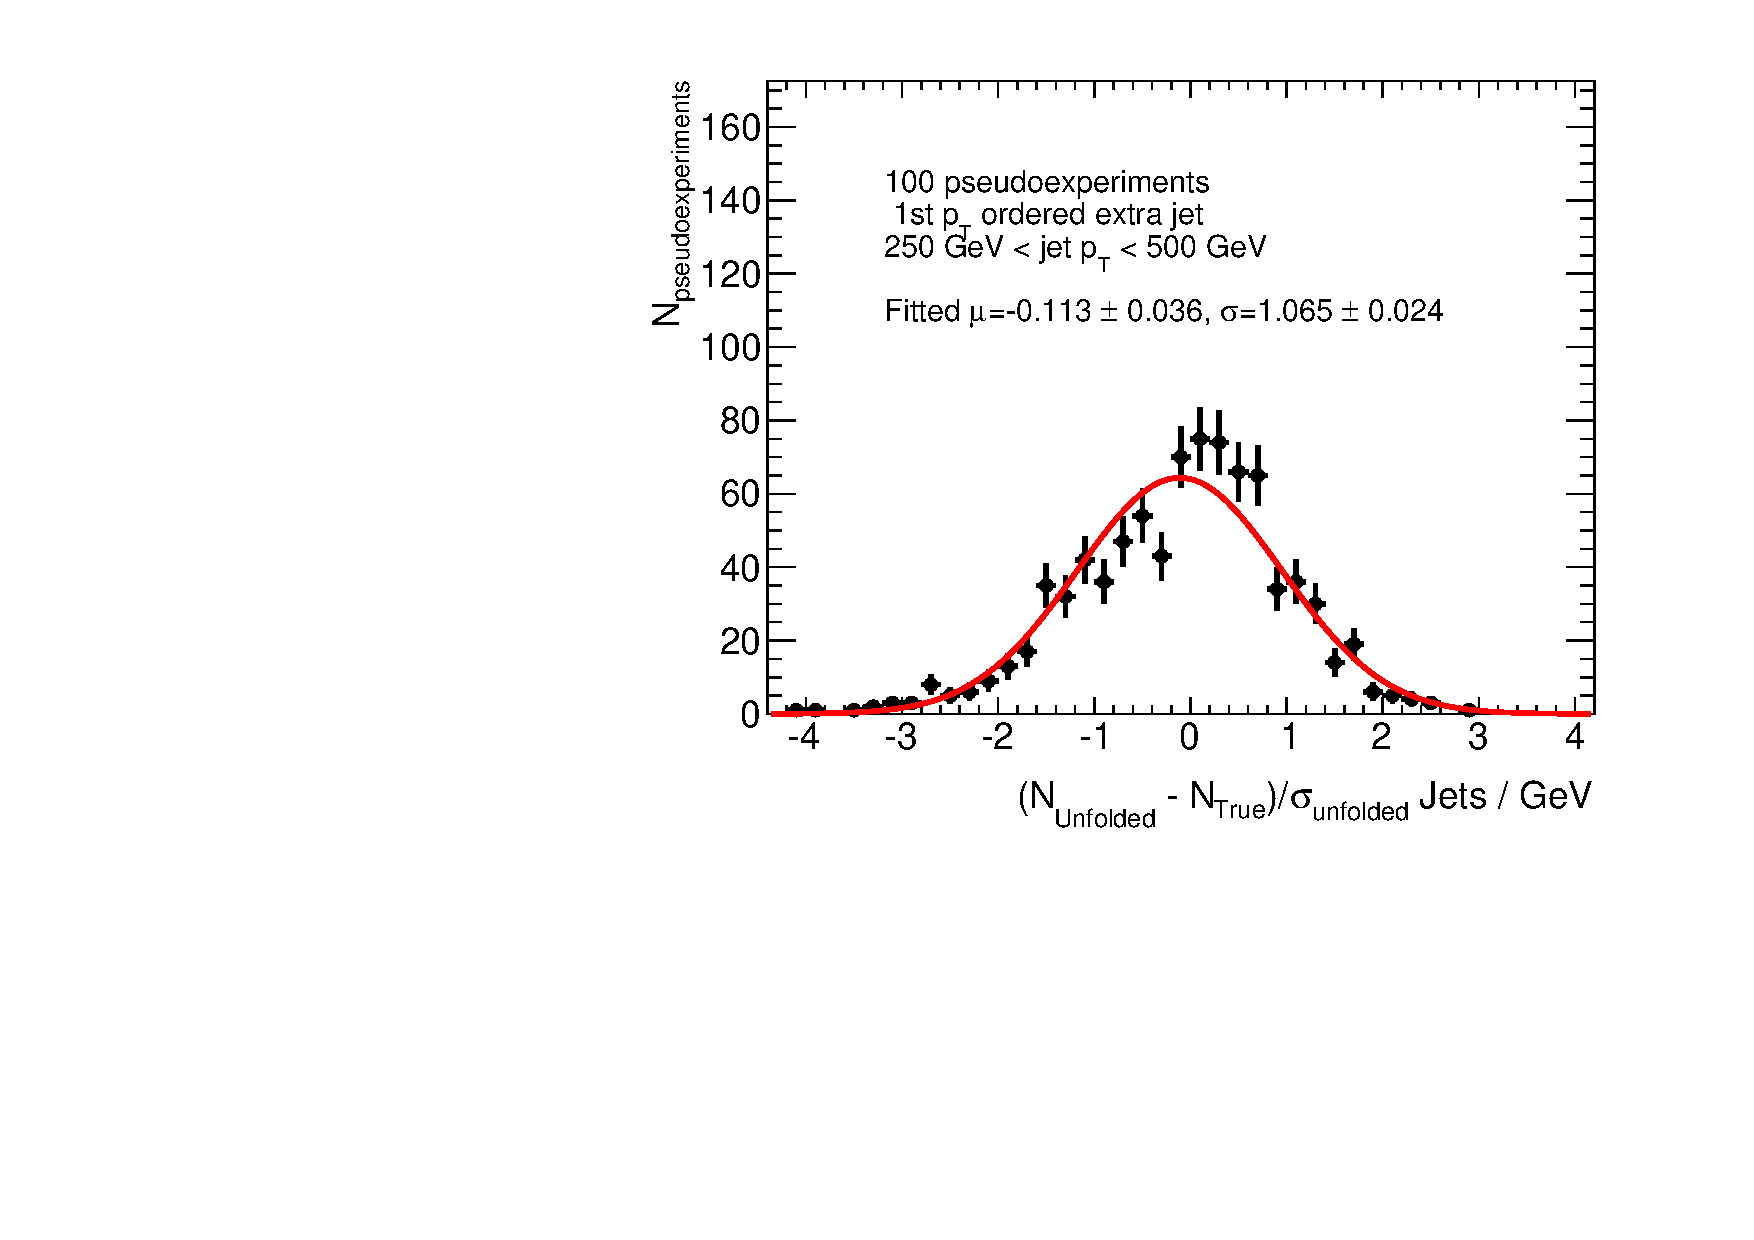
\includegraphics[width=0.33\textwidth]{fig/UnfoldPull/SingleSlicePull16.pdf}
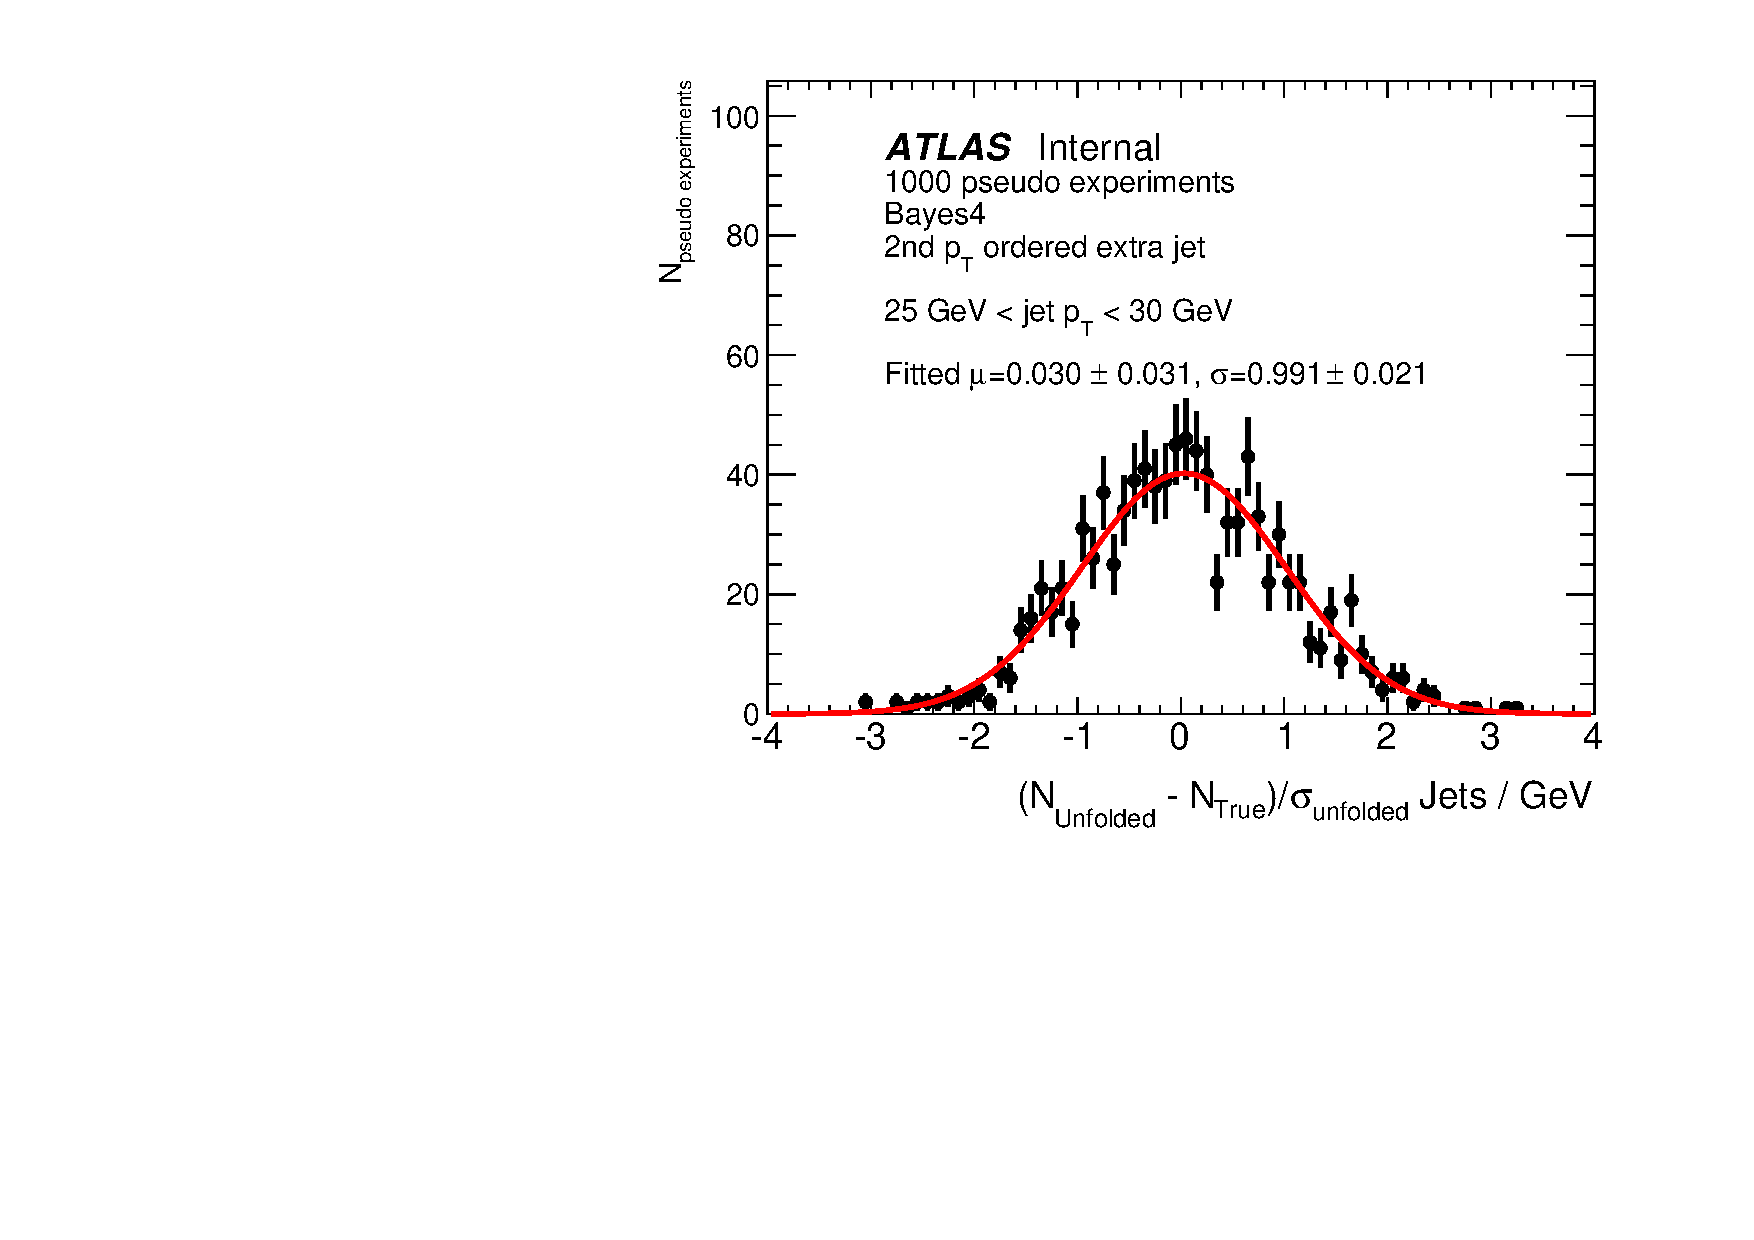
\includegraphics[width=0.33\textwidth]{fig/UnfoldPull/SingleSlicePull17.pdf}
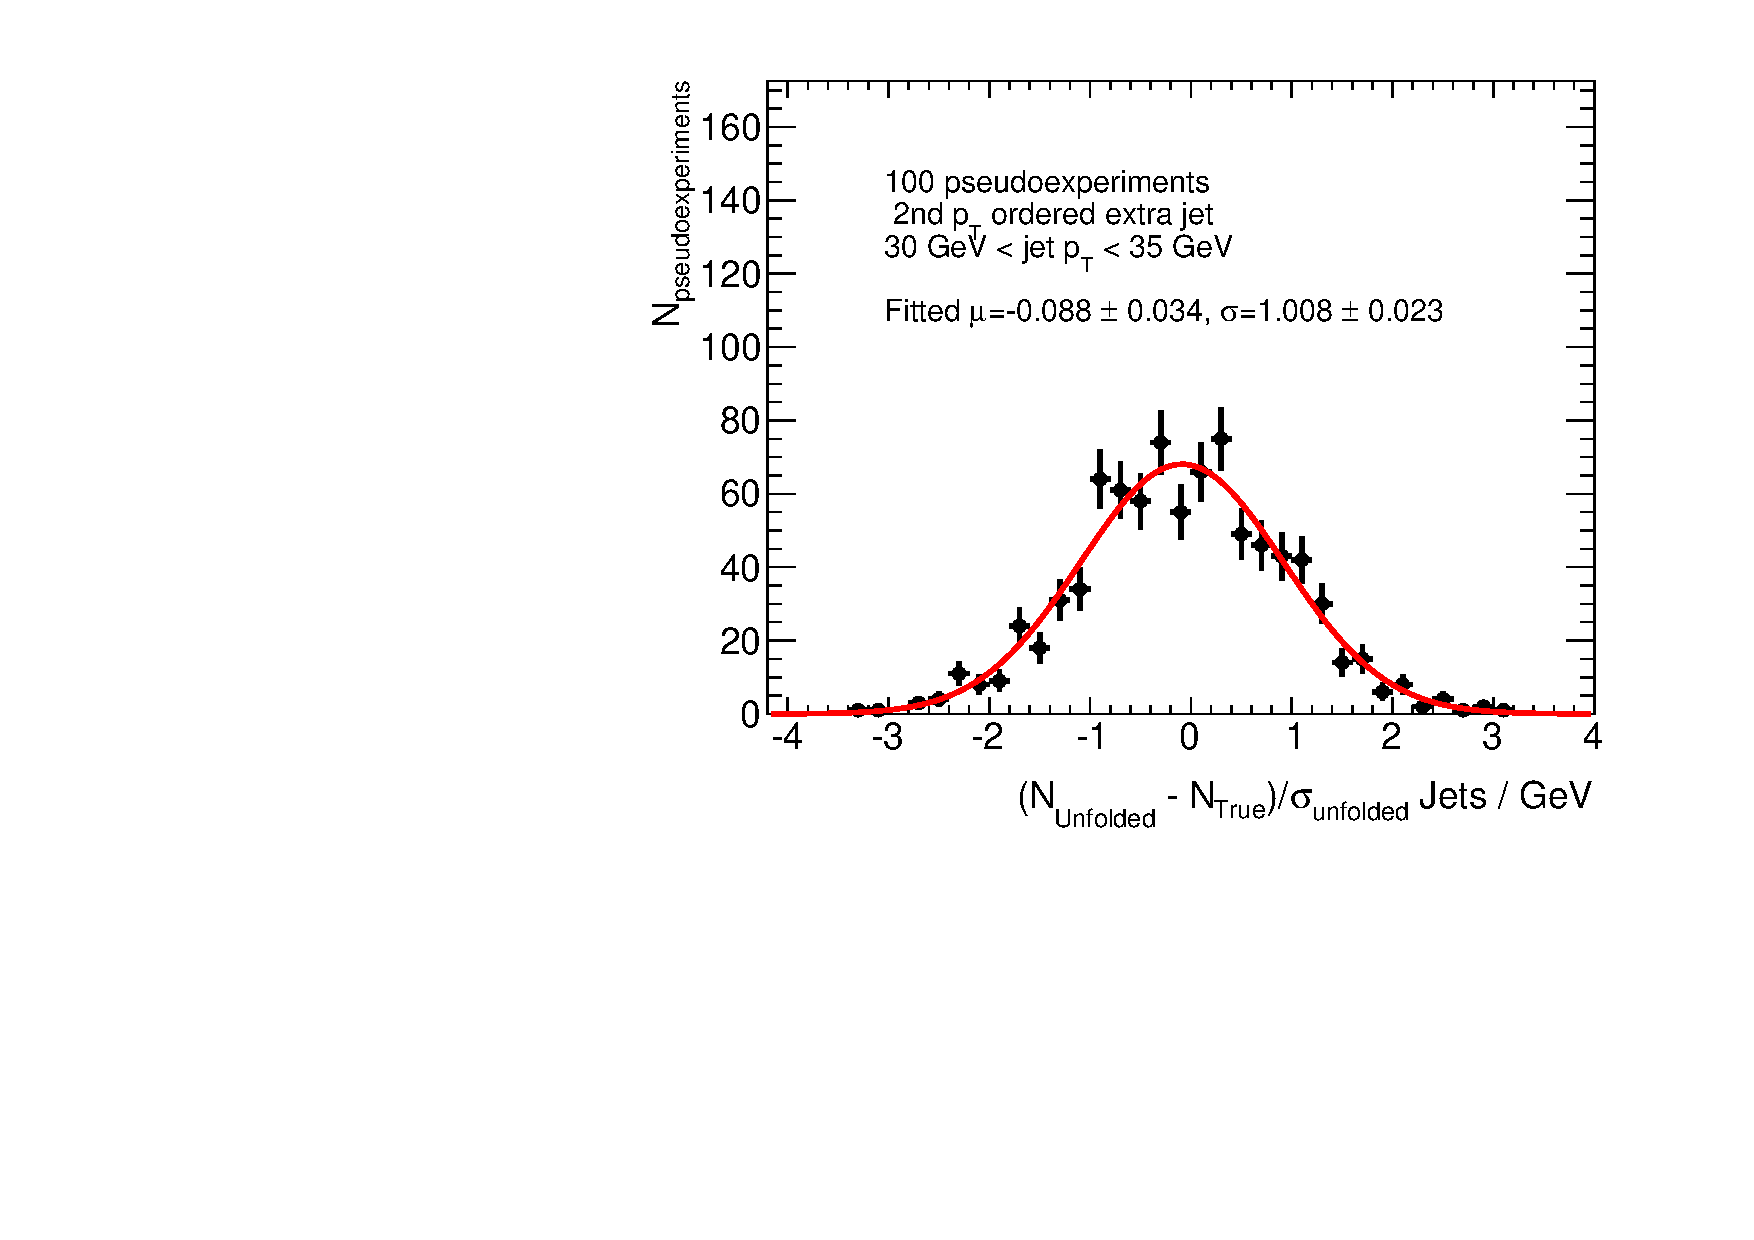
\includegraphics[width=0.33\textwidth]{fig/UnfoldPull/SingleSlicePull18.pdf}
%
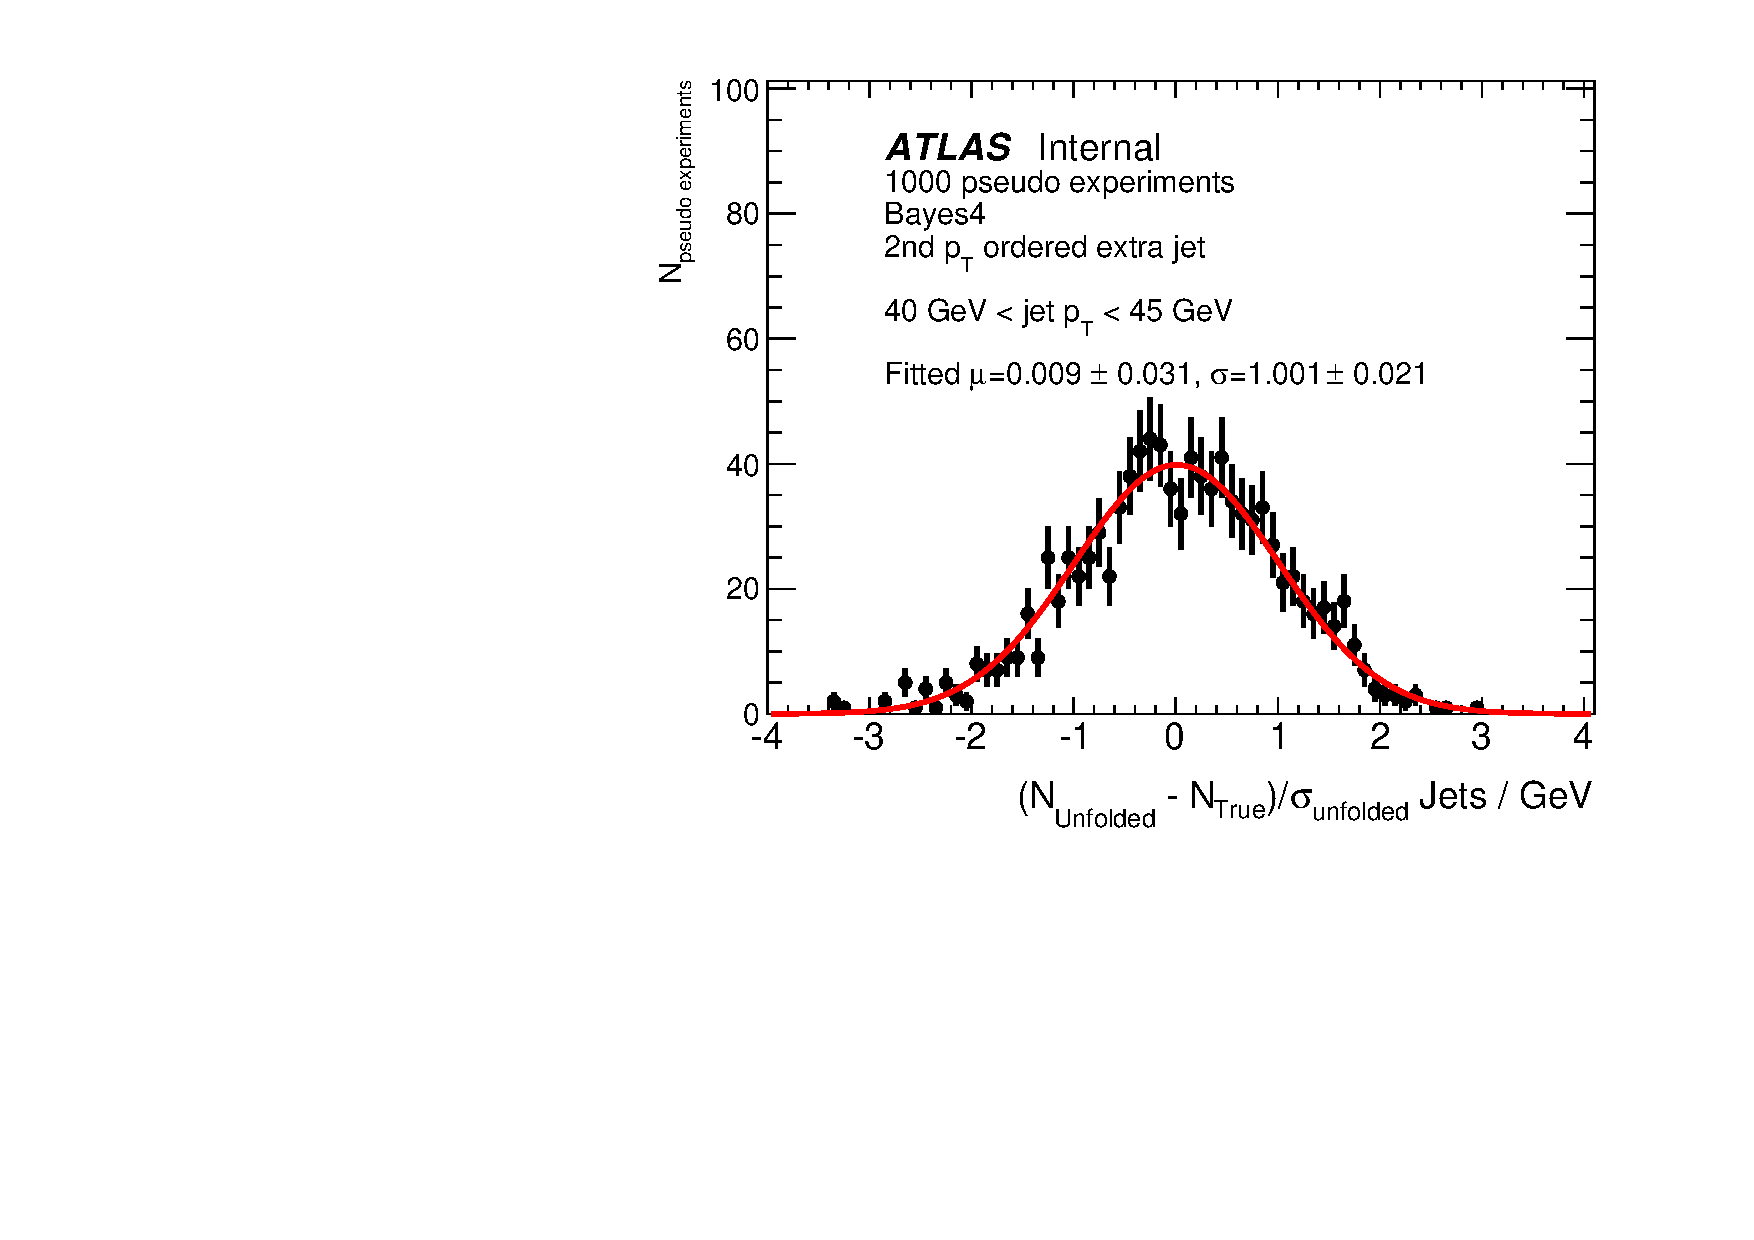
\includegraphics[width=0.33\textwidth]{fig/UnfoldPull/SingleSlicePull20.pdf}
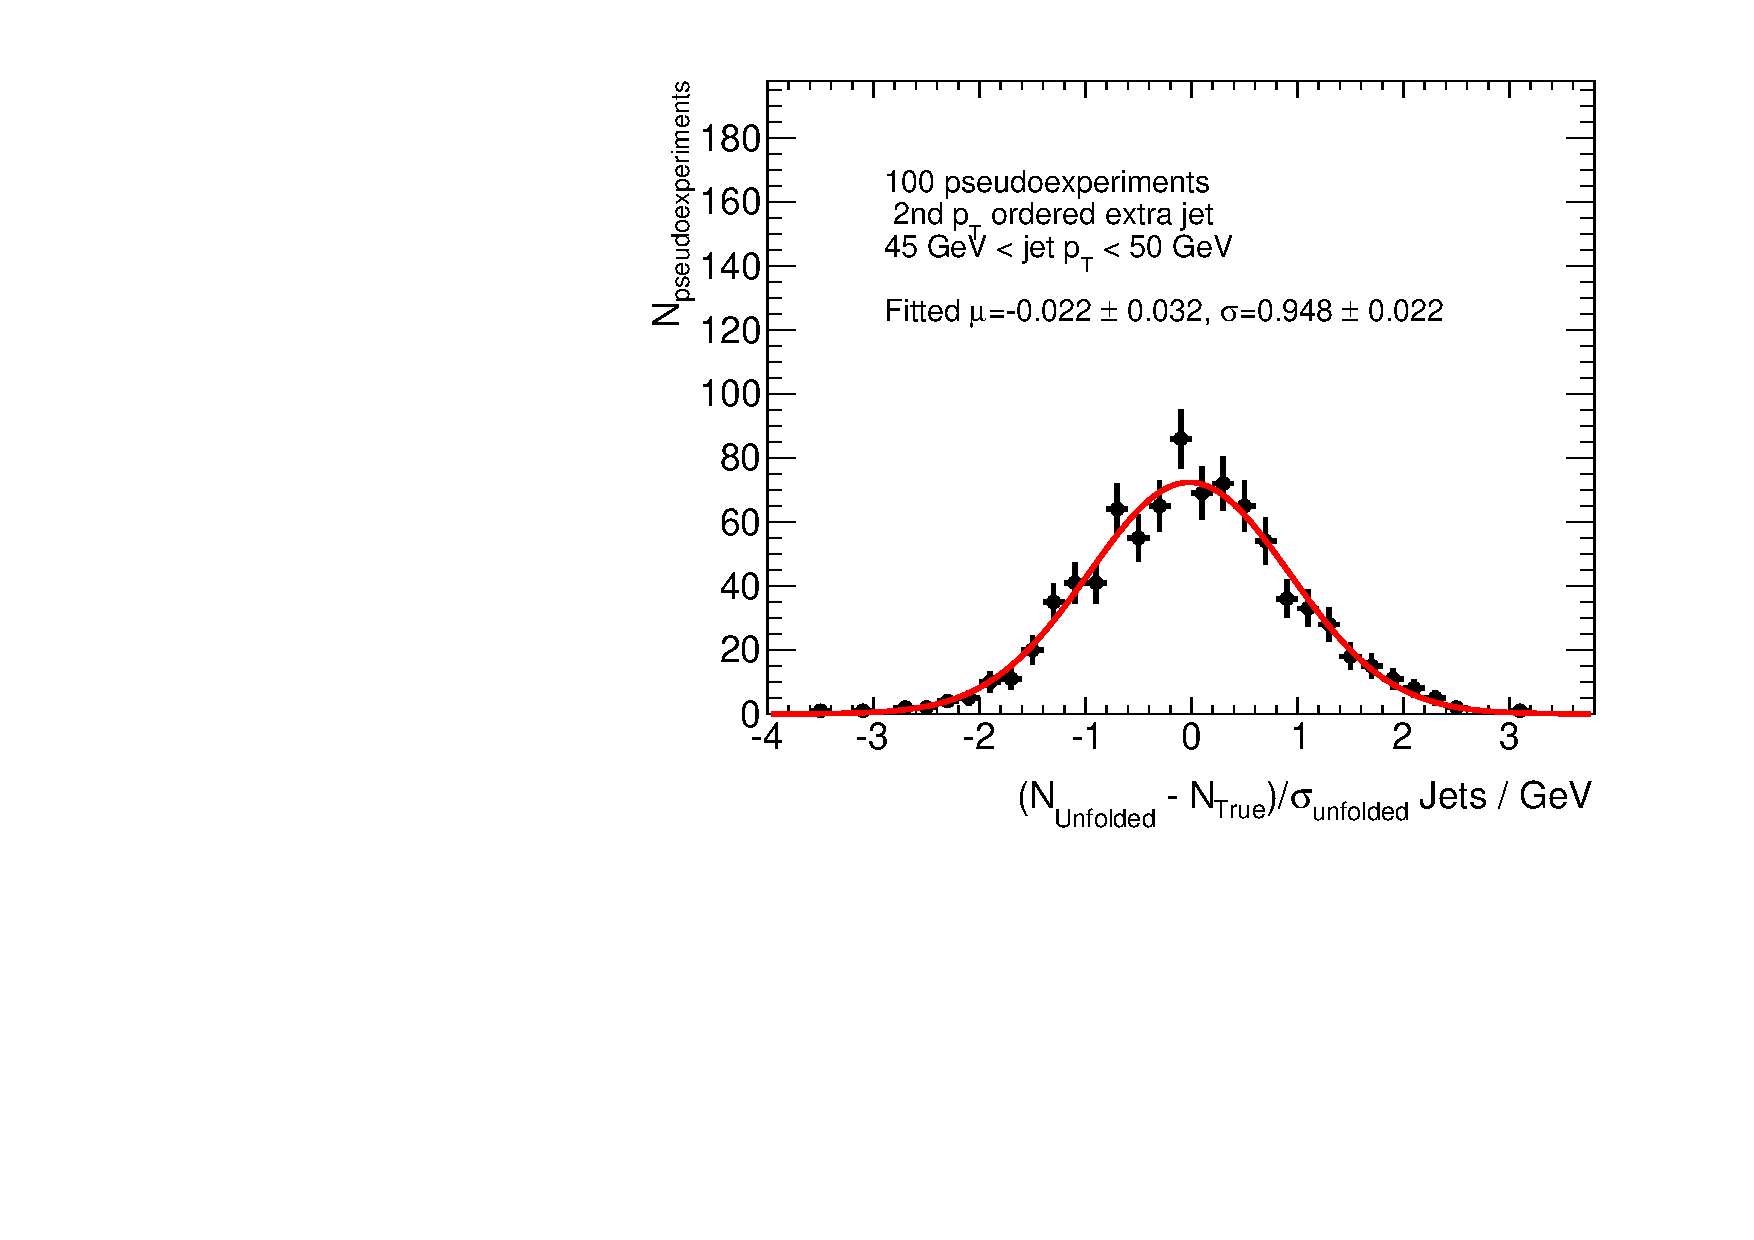
\includegraphics[width=0.33\textwidth]{fig/UnfoldPull/SingleSlicePull21.pdf}
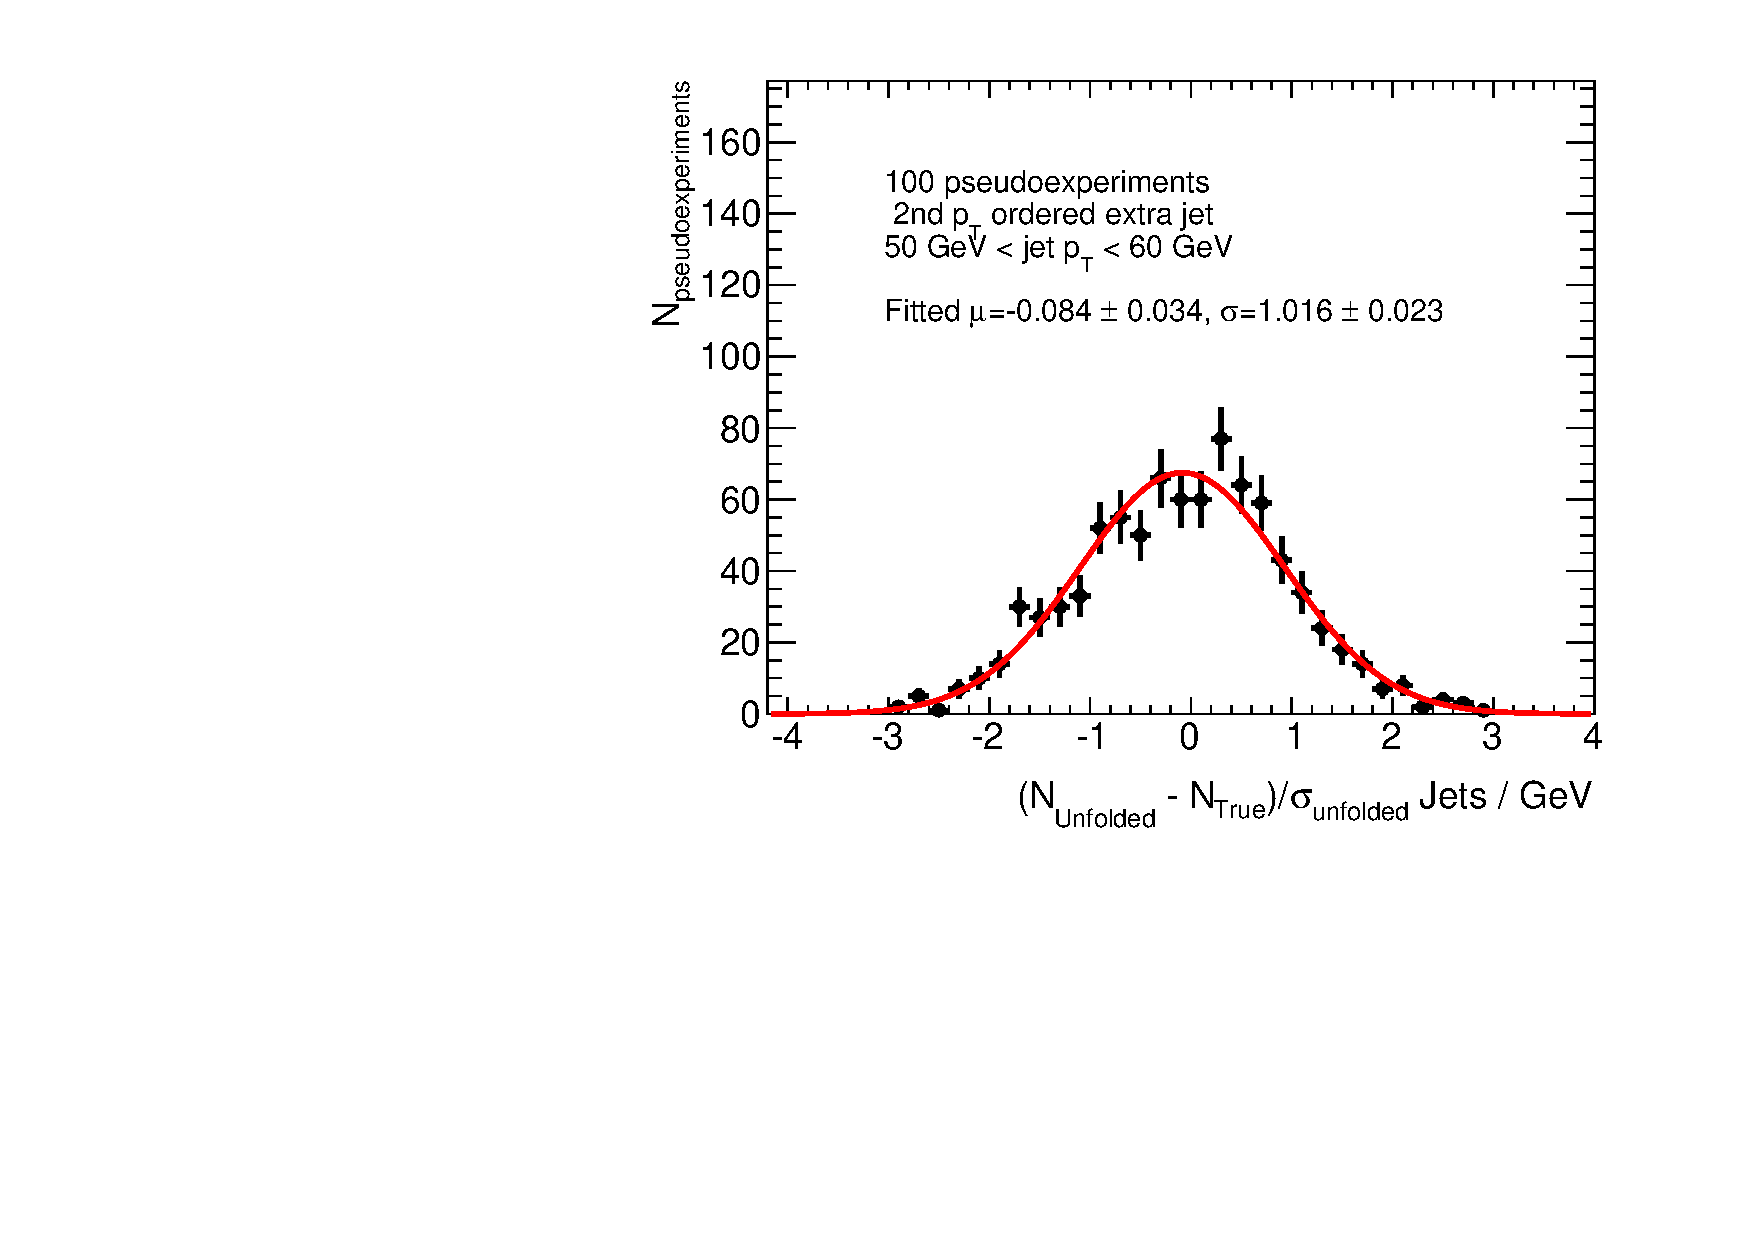
\includegraphics[width=0.33\textwidth]{fig/UnfoldPull/SingleSlicePull22.pdf}
%
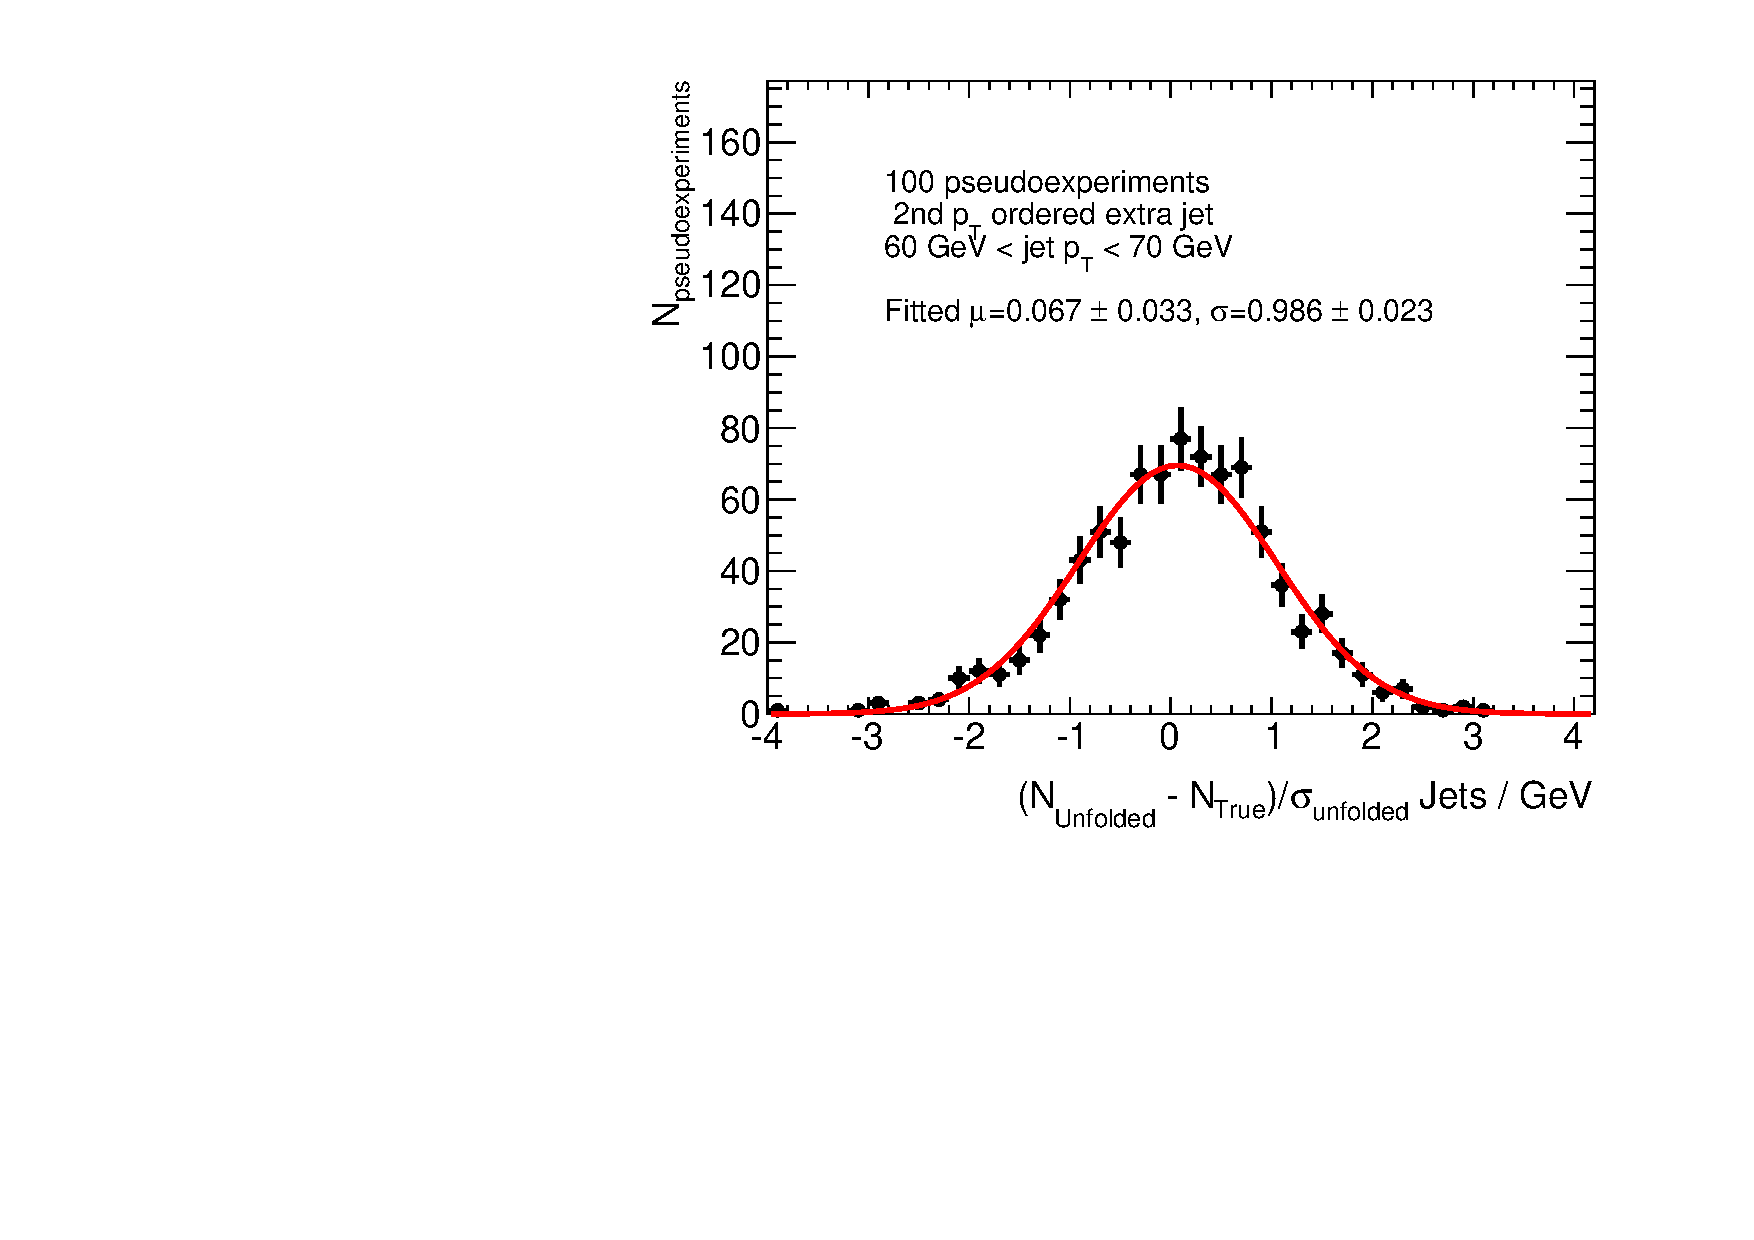
\includegraphics[width=0.33\textwidth]{fig/UnfoldPull/SingleSlicePull23.pdf}
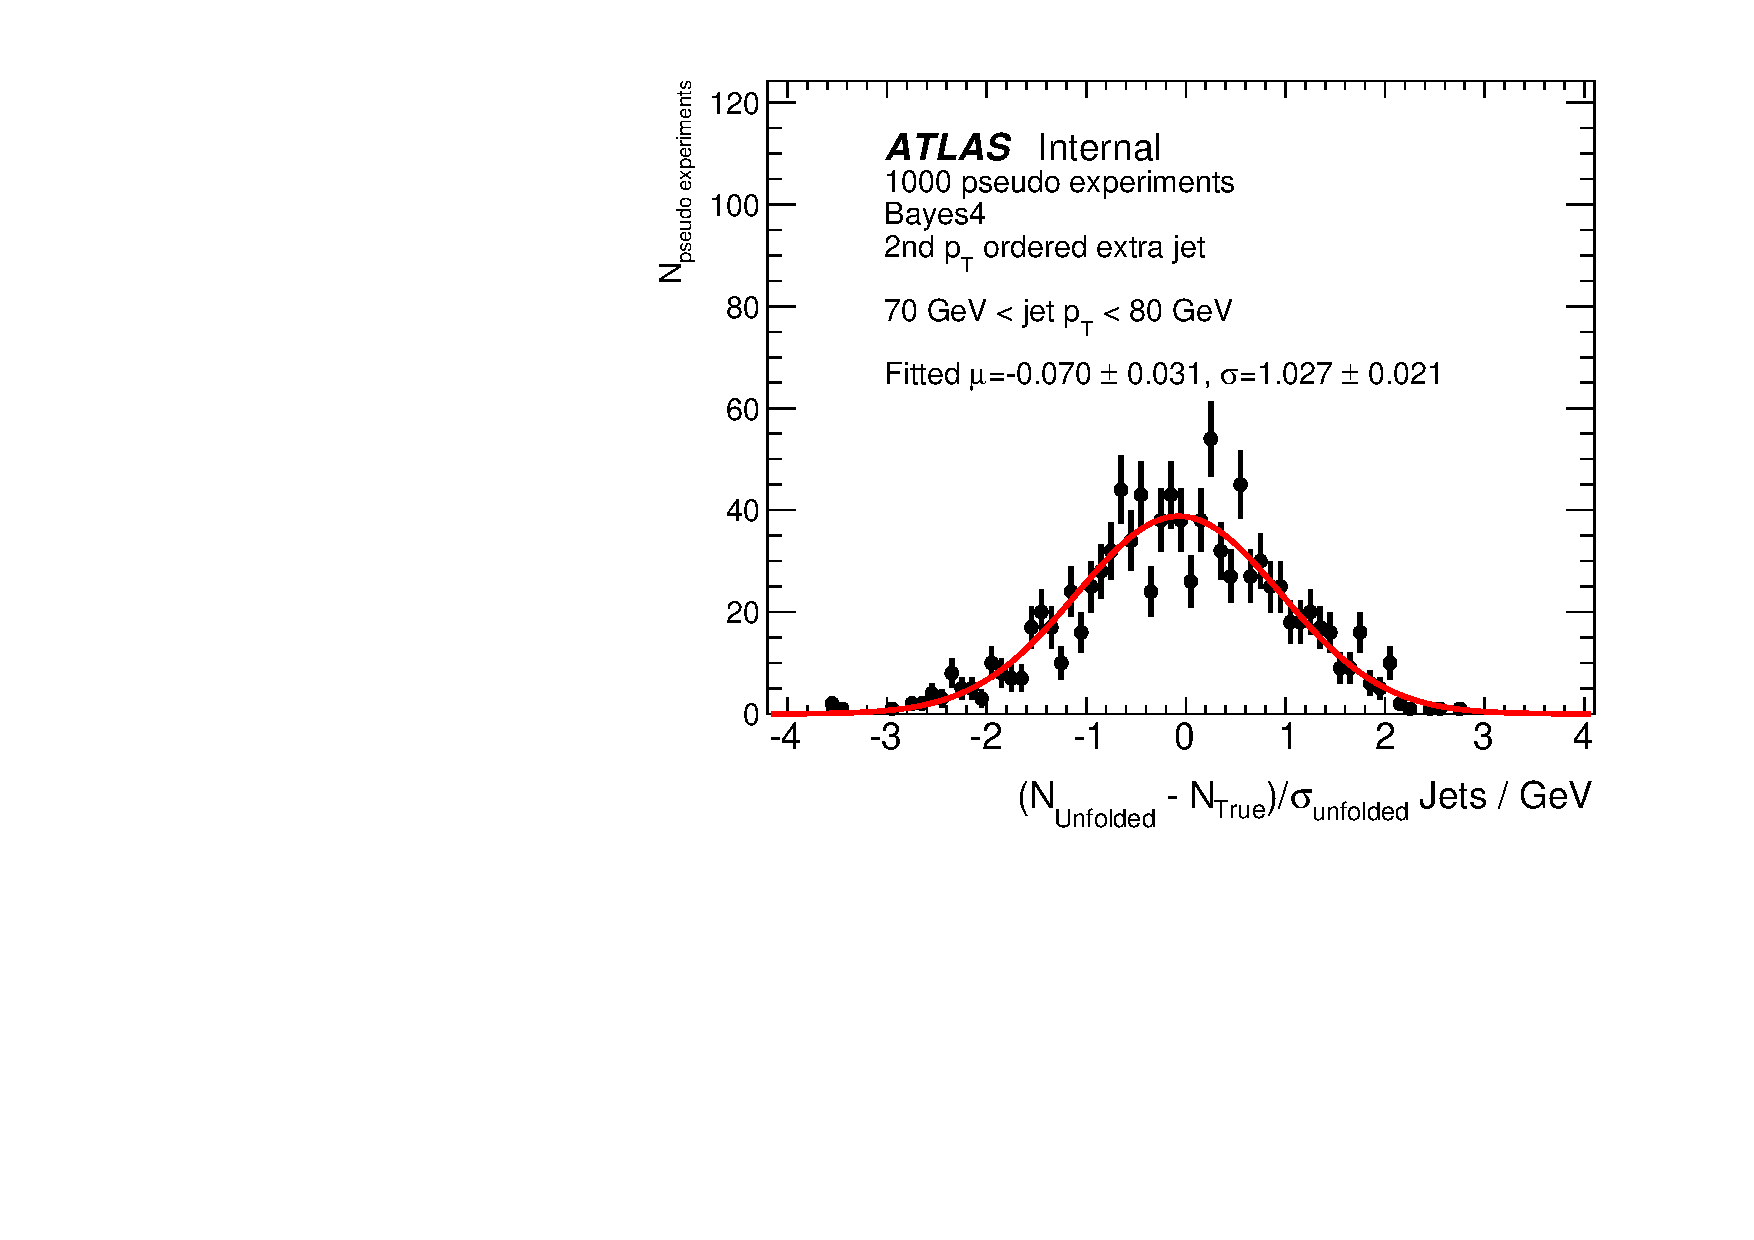
\includegraphics[width=0.33\textwidth]{fig/UnfoldPull/SingleSlicePull24.pdf}
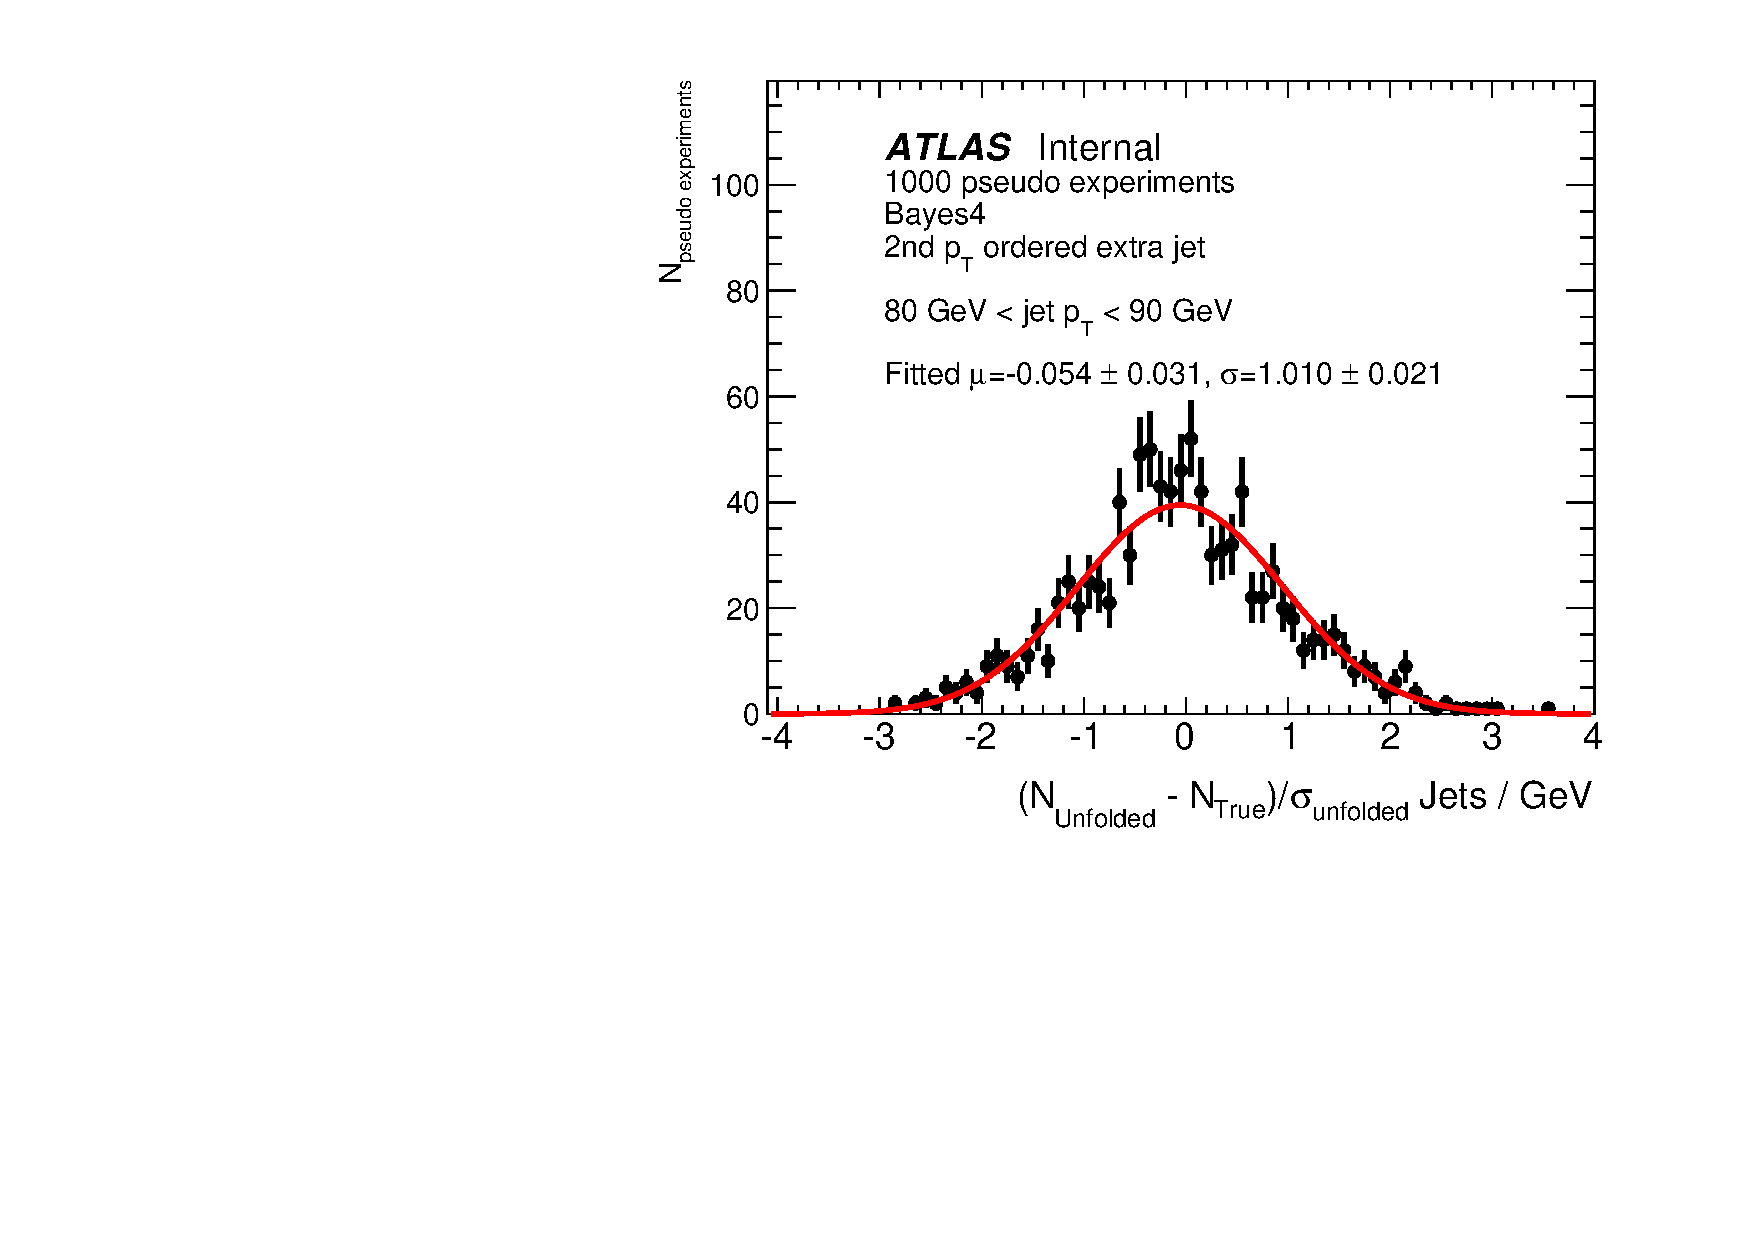
\includegraphics[width=0.33\textwidth]{fig/UnfoldPull/SingleSlicePull25.pdf}
%
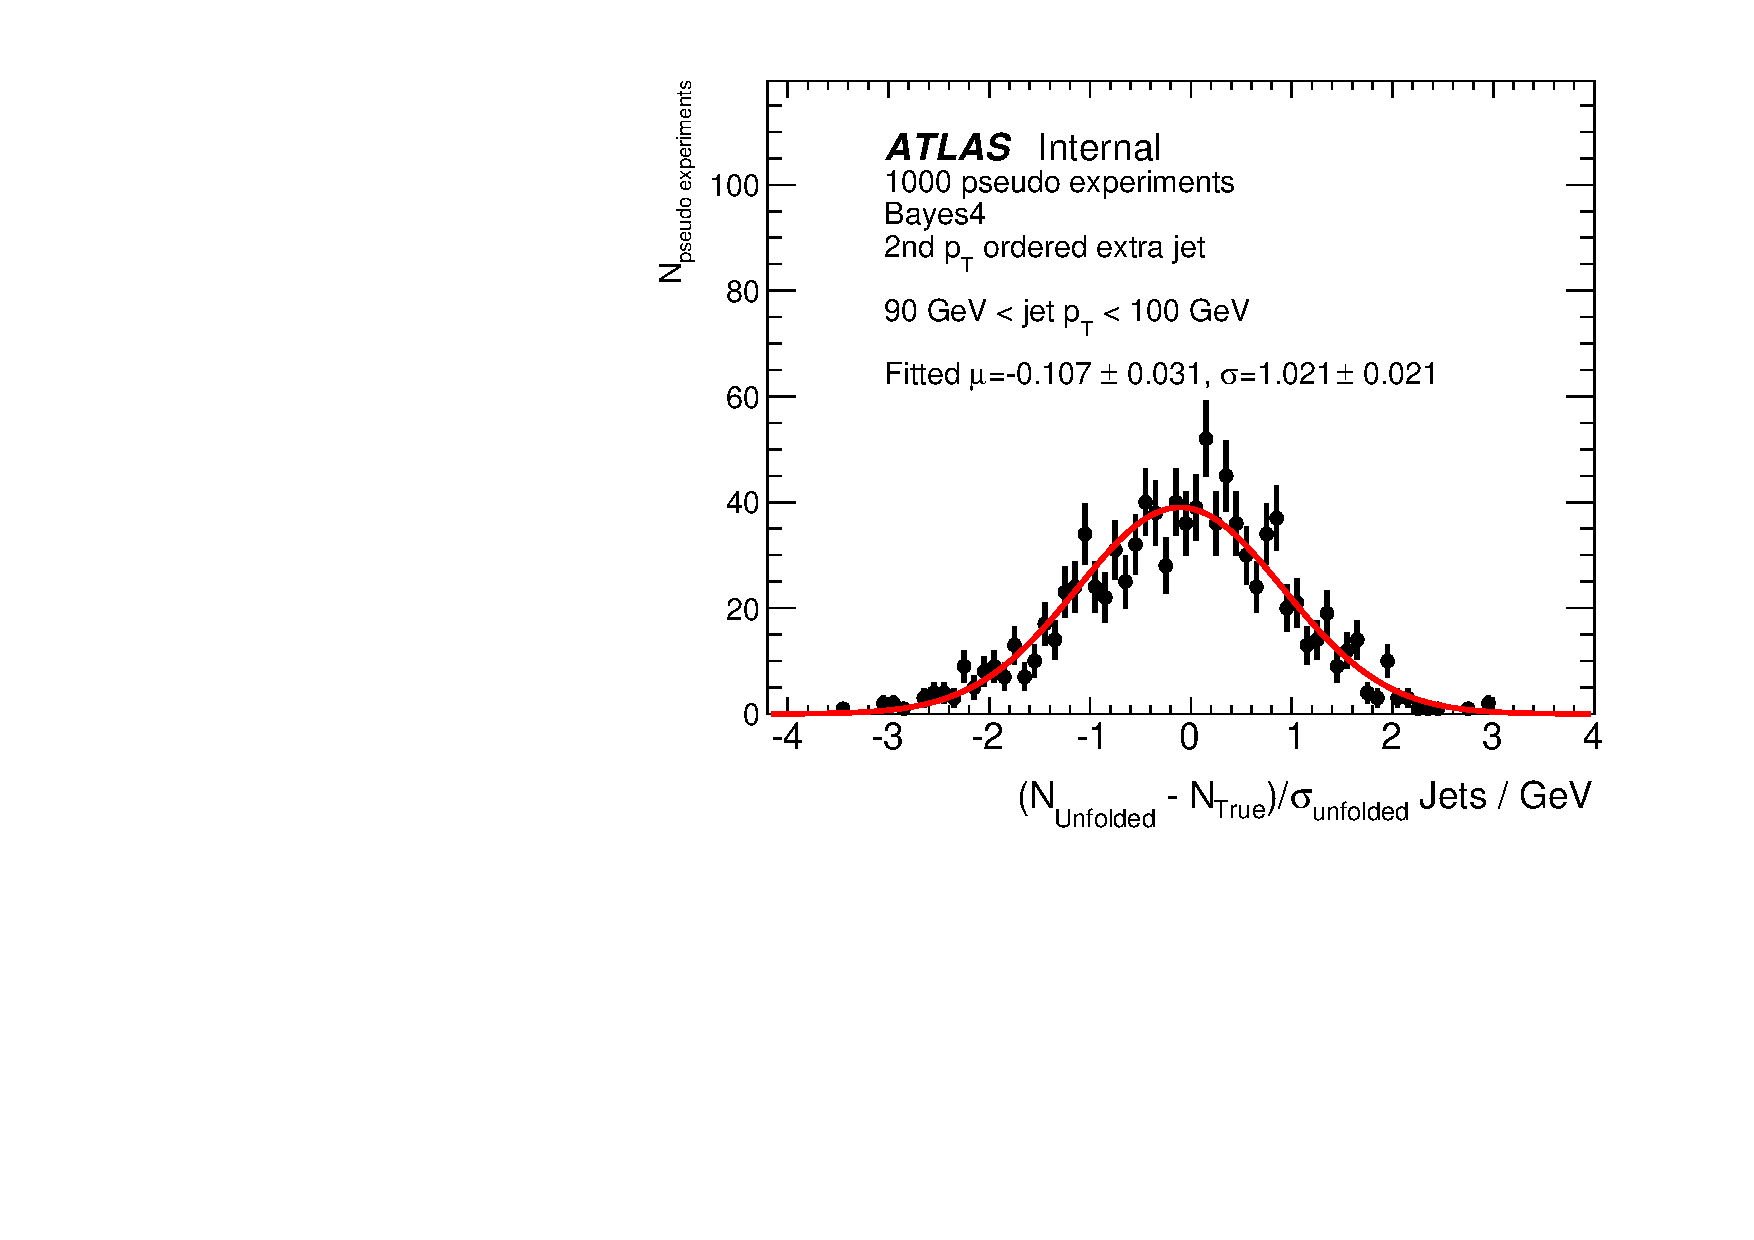
\includegraphics[width=0.33\textwidth]{fig/UnfoldPull/SingleSlicePull26.pdf}
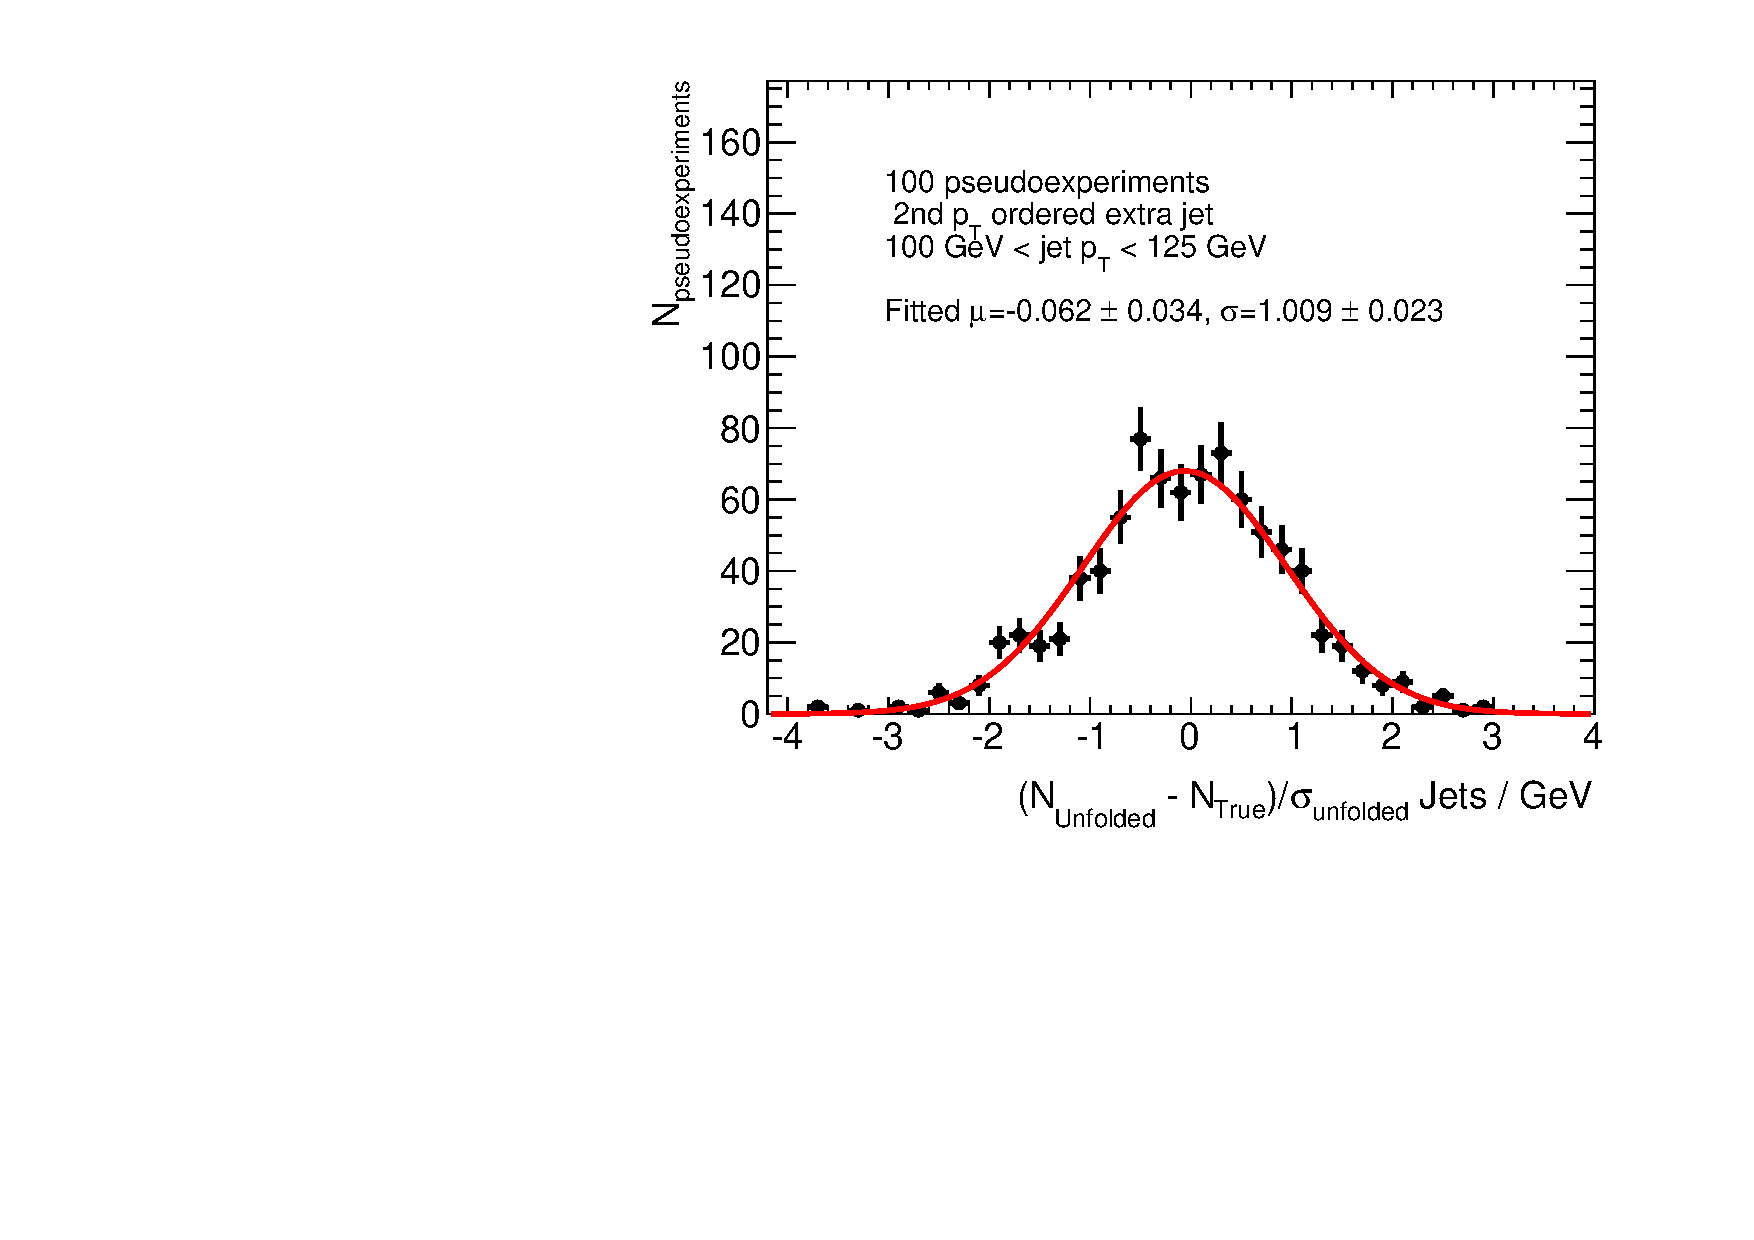
\includegraphics[width=0.33\textwidth]{fig/UnfoldPull/SingleSlicePull27.pdf}
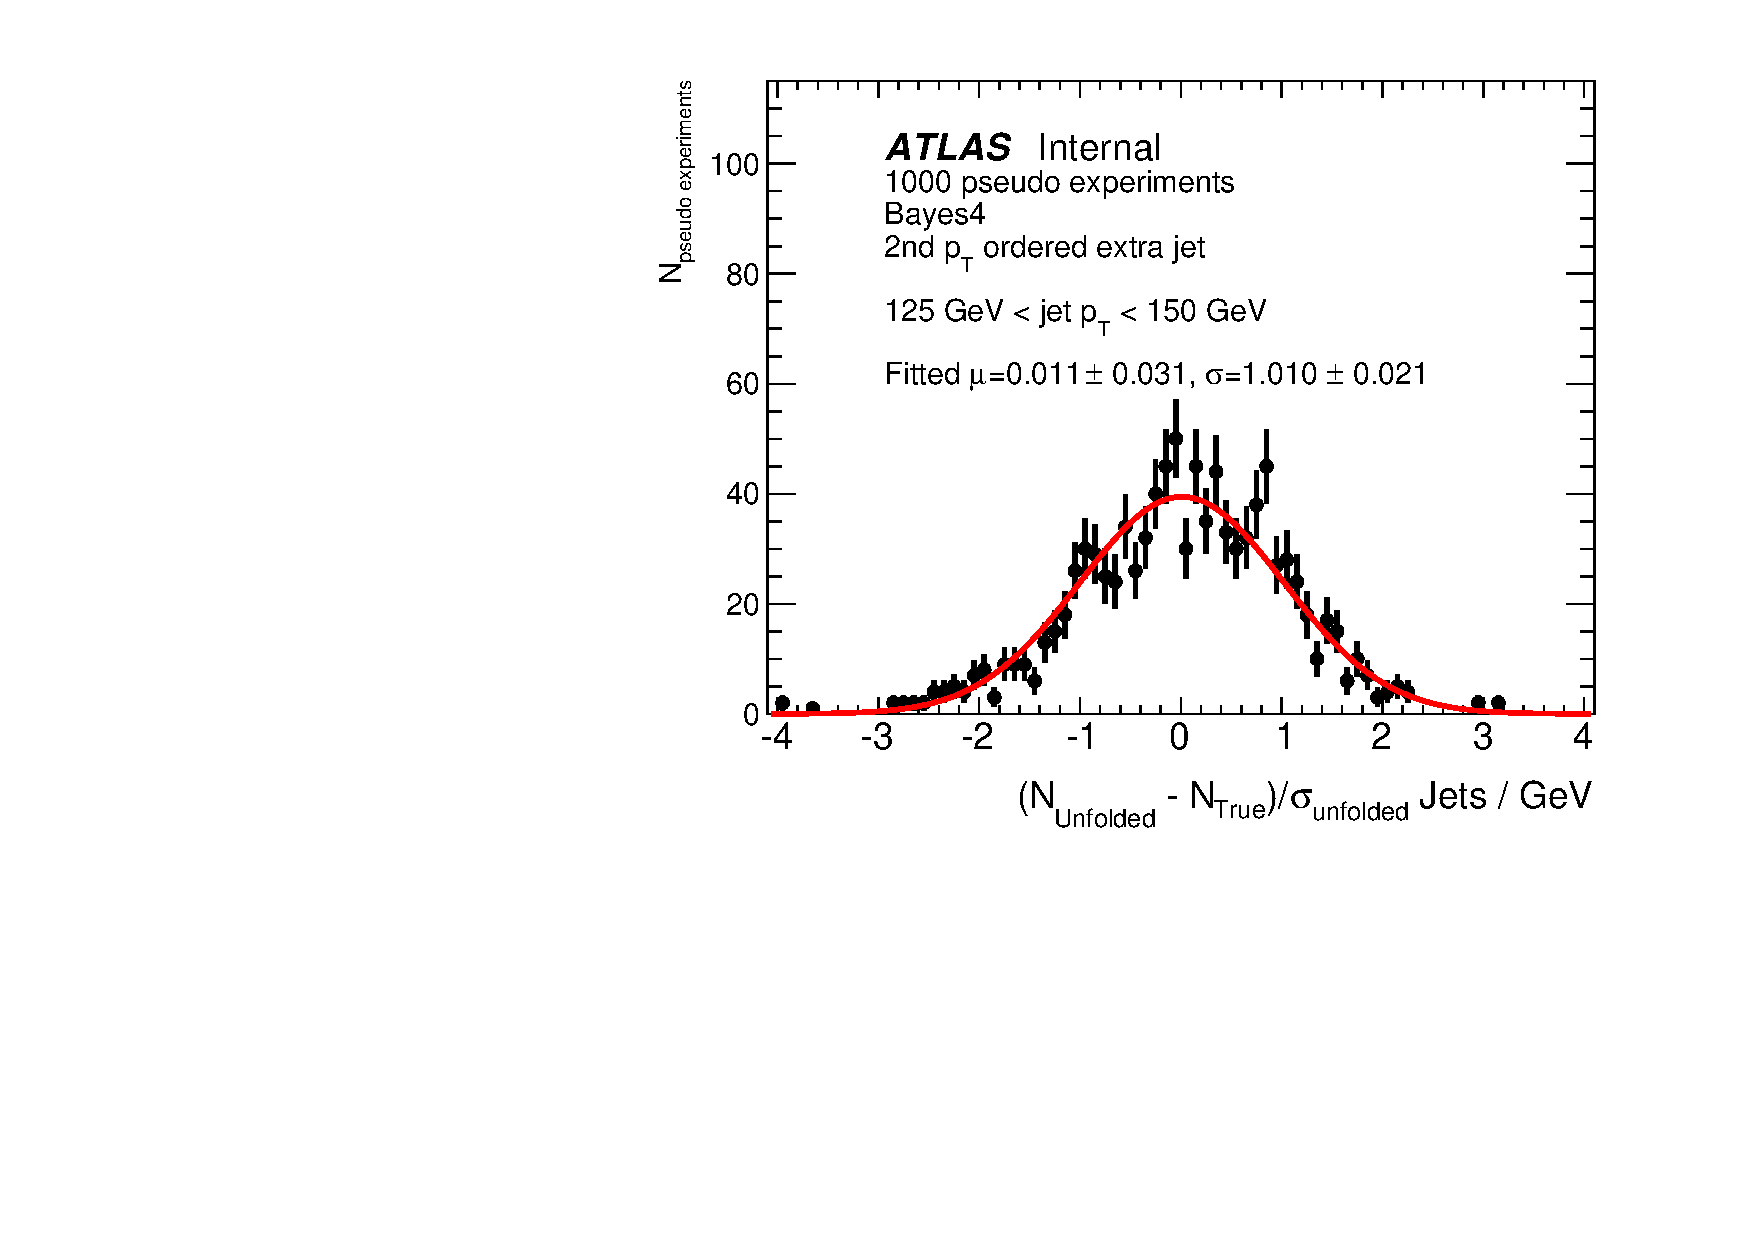
\includegraphics[width=0.33\textwidth]{fig/UnfoldPull/SingleSlicePull28.pdf}
%
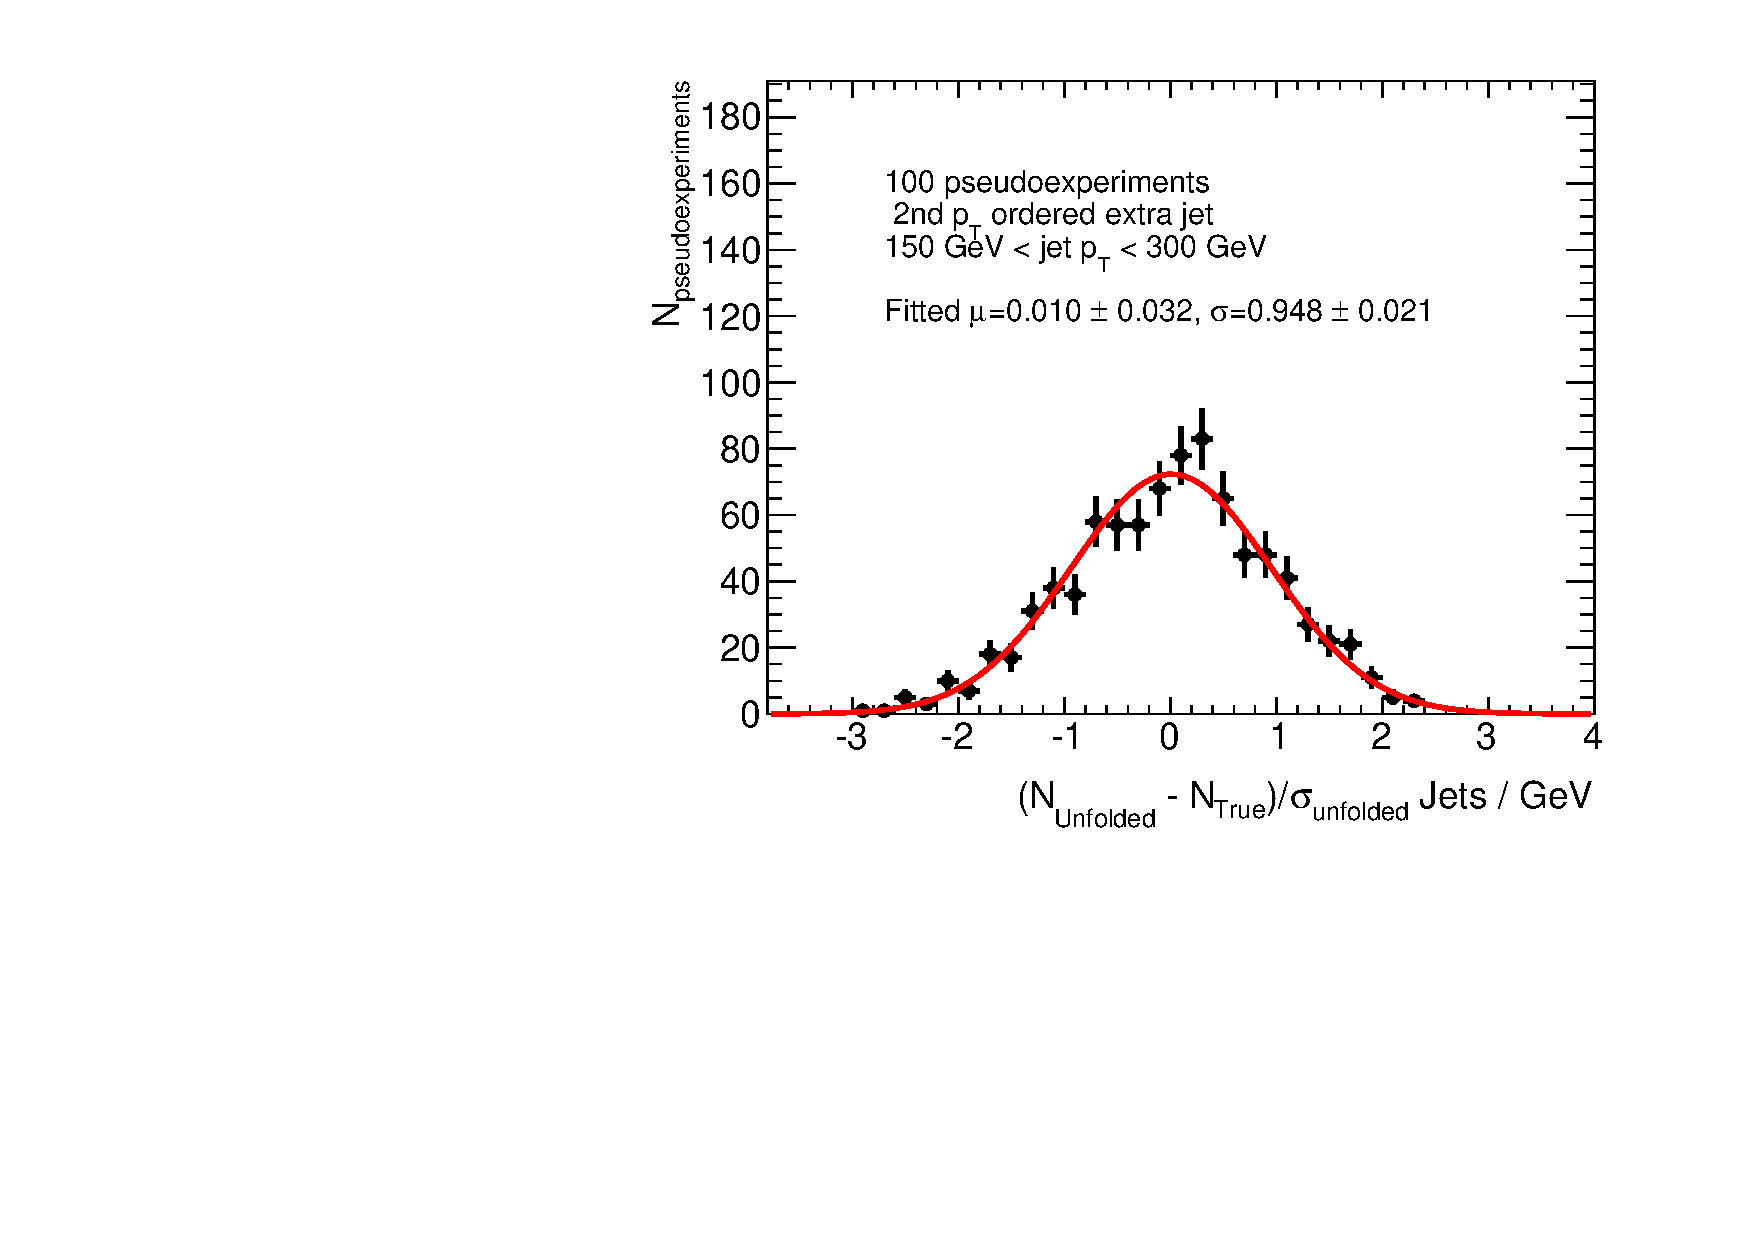
\includegraphics[width=0.33\textwidth]{fig/UnfoldPull/SingleSlicePull29.pdf}
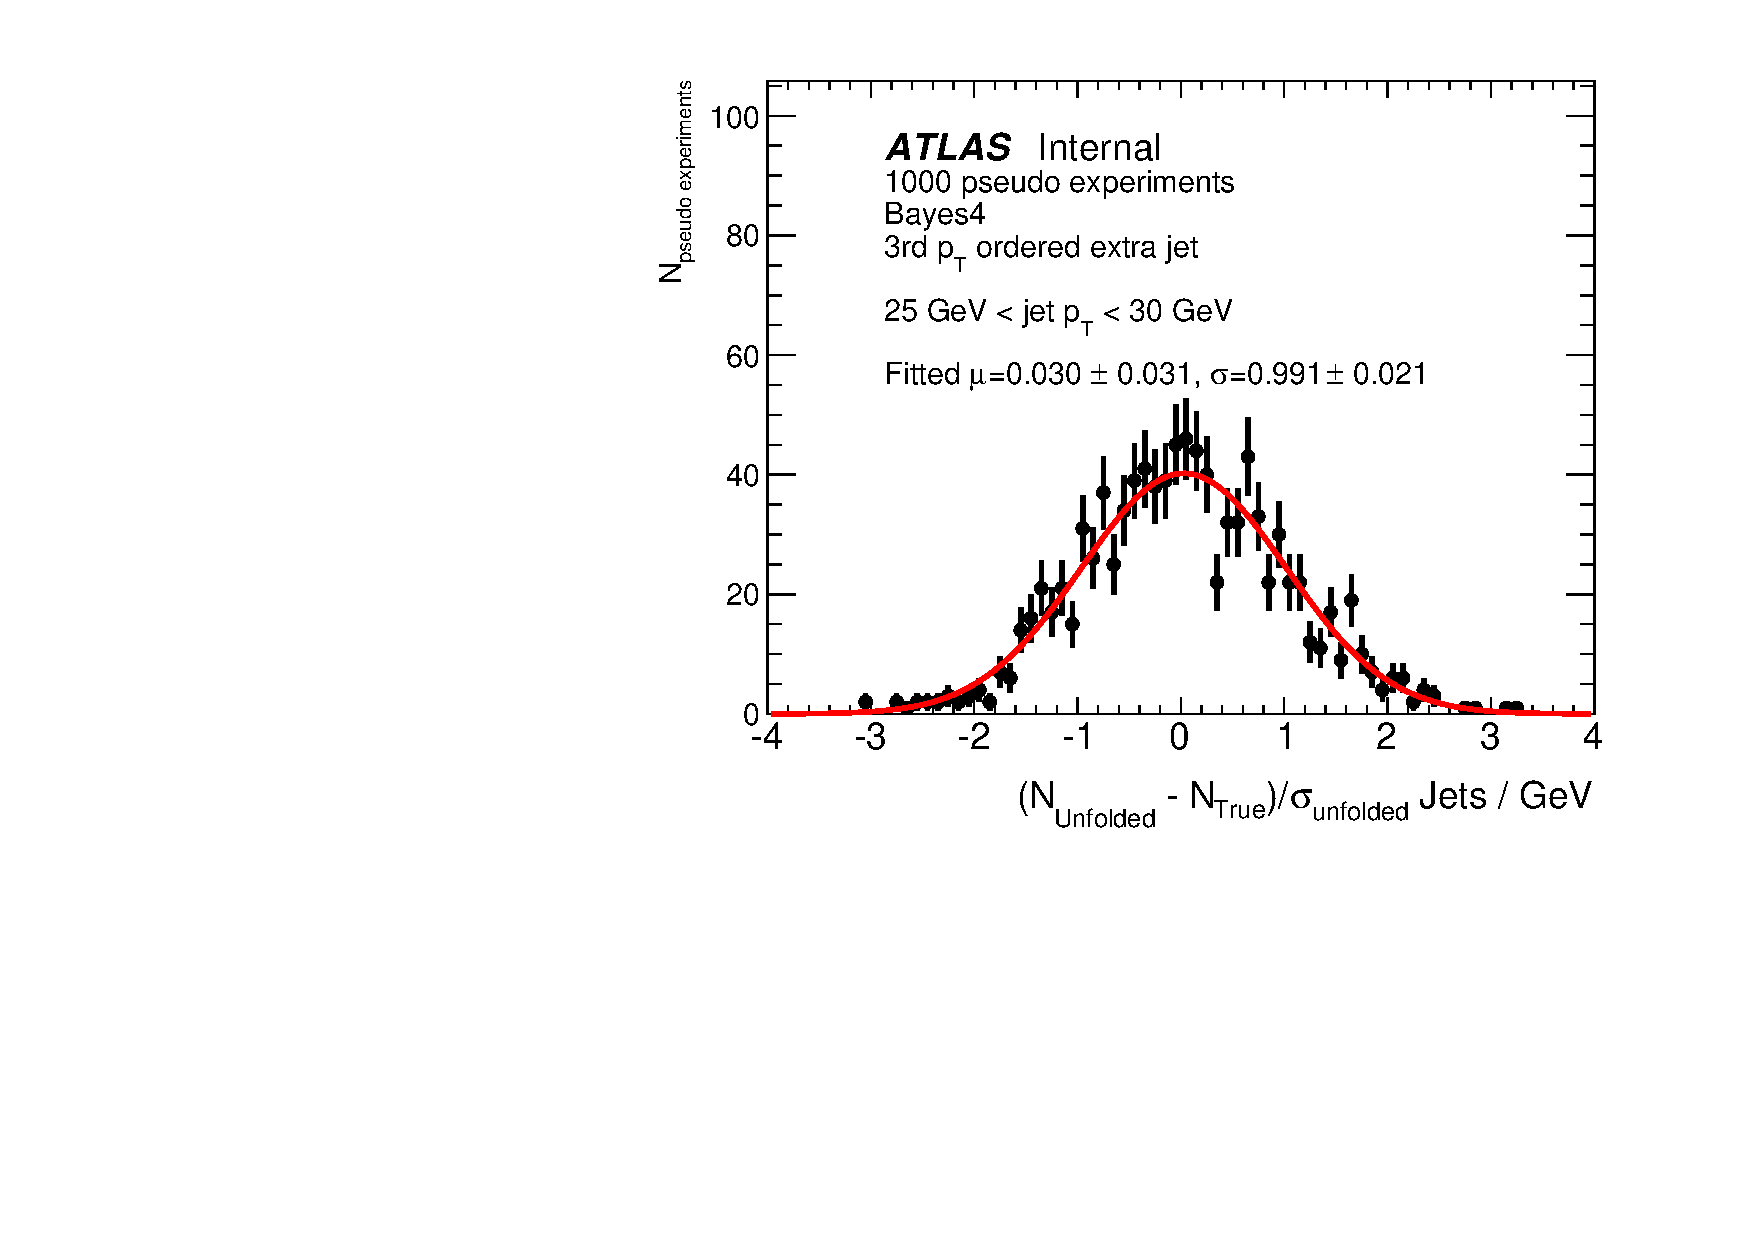
\includegraphics[width=0.33\textwidth]{fig/UnfoldPull/SingleSlicePull30.pdf}
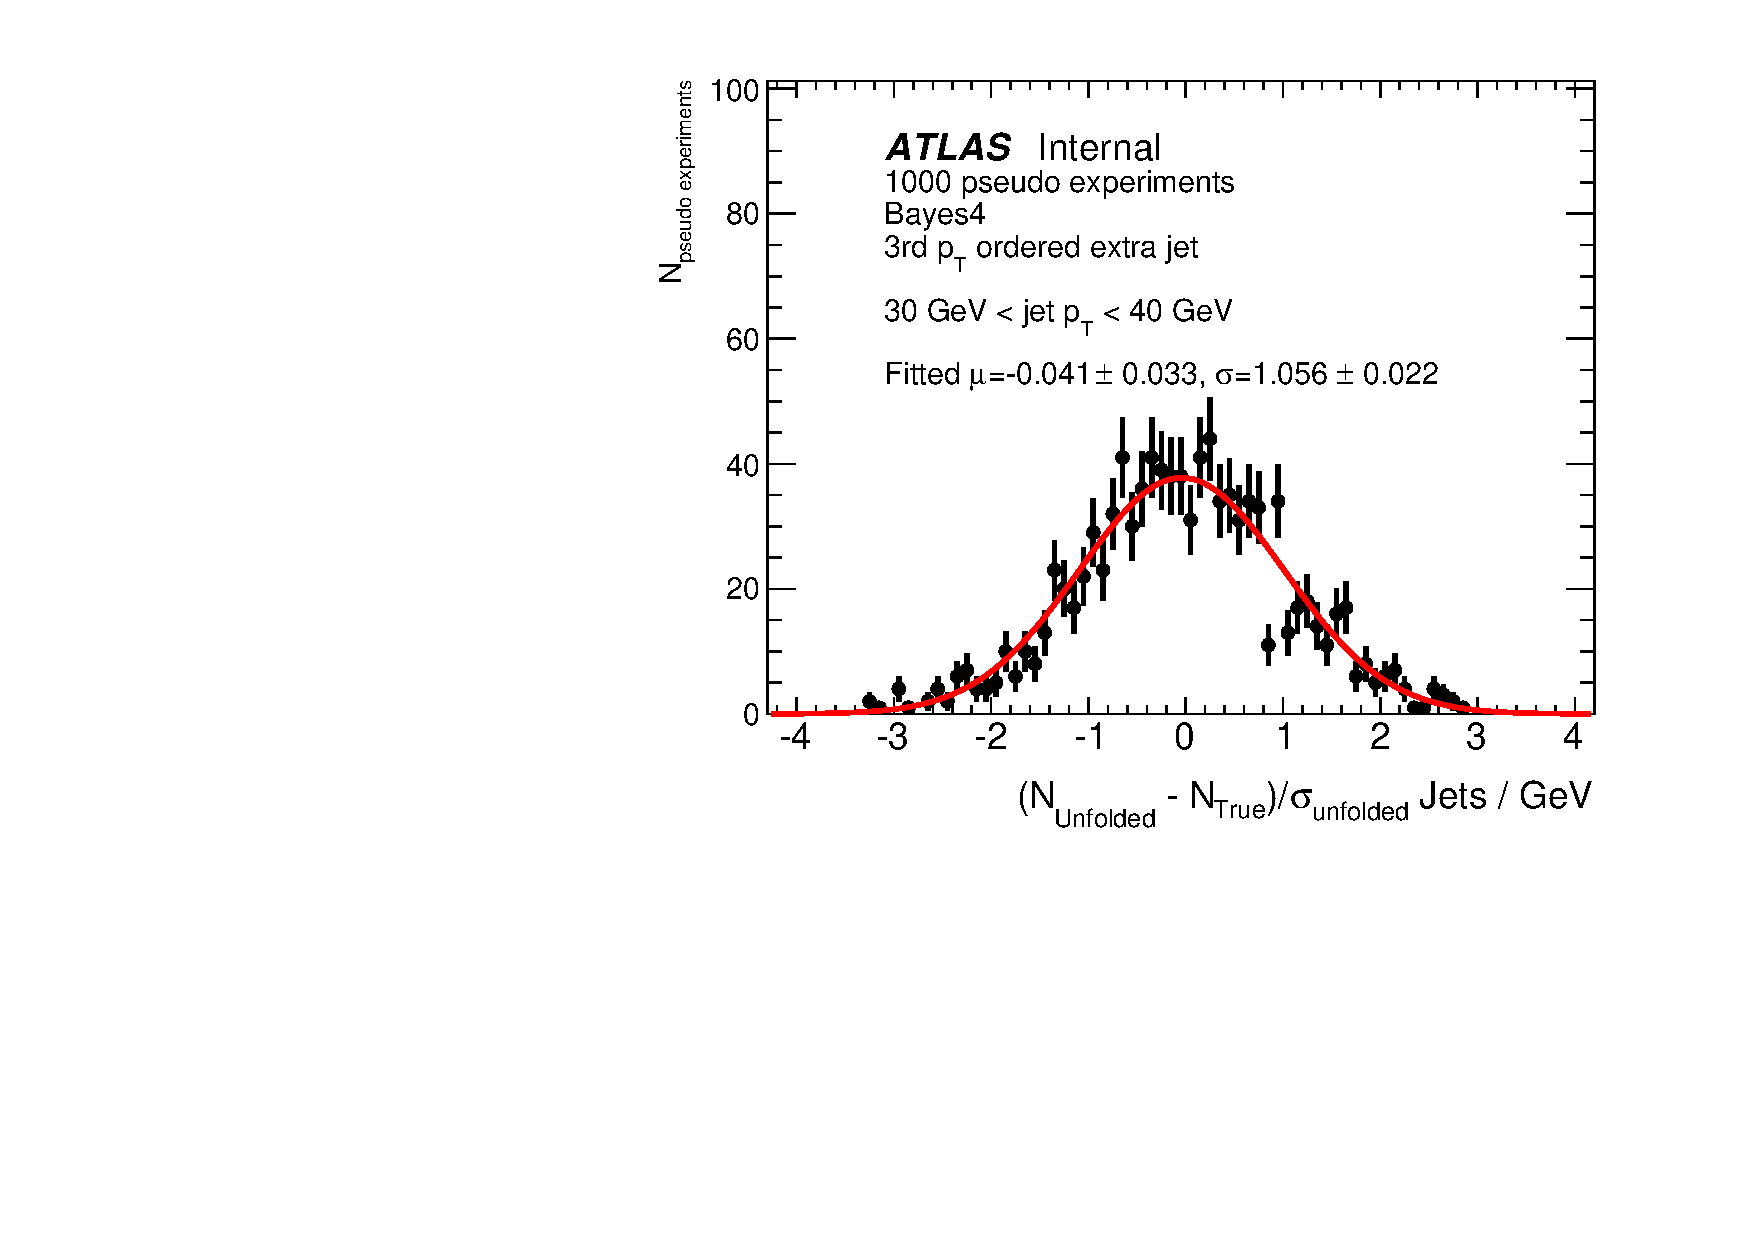
\includegraphics[width=0.33\textwidth]{fig/UnfoldPull/SingleSlicePull31.pdf}
%
\caption{Pull distributions for the extra jets from the baseline \ttbar\ +Wt simulation (\powpy) unfolded against a matrix filled with the baseline \ttbar\ +Wt simulation (\powpy). The Bayesian unfolding method 4 iterations is used. One thousand pseudoexperiments, each the size of the events in data, are randomly selected from the sample and unfolded.  A Gaussian is fit to the distributions of biases over the pseudoexperiments.}
\label{fig:appPull1}
\end{figure}
\begin{figure}
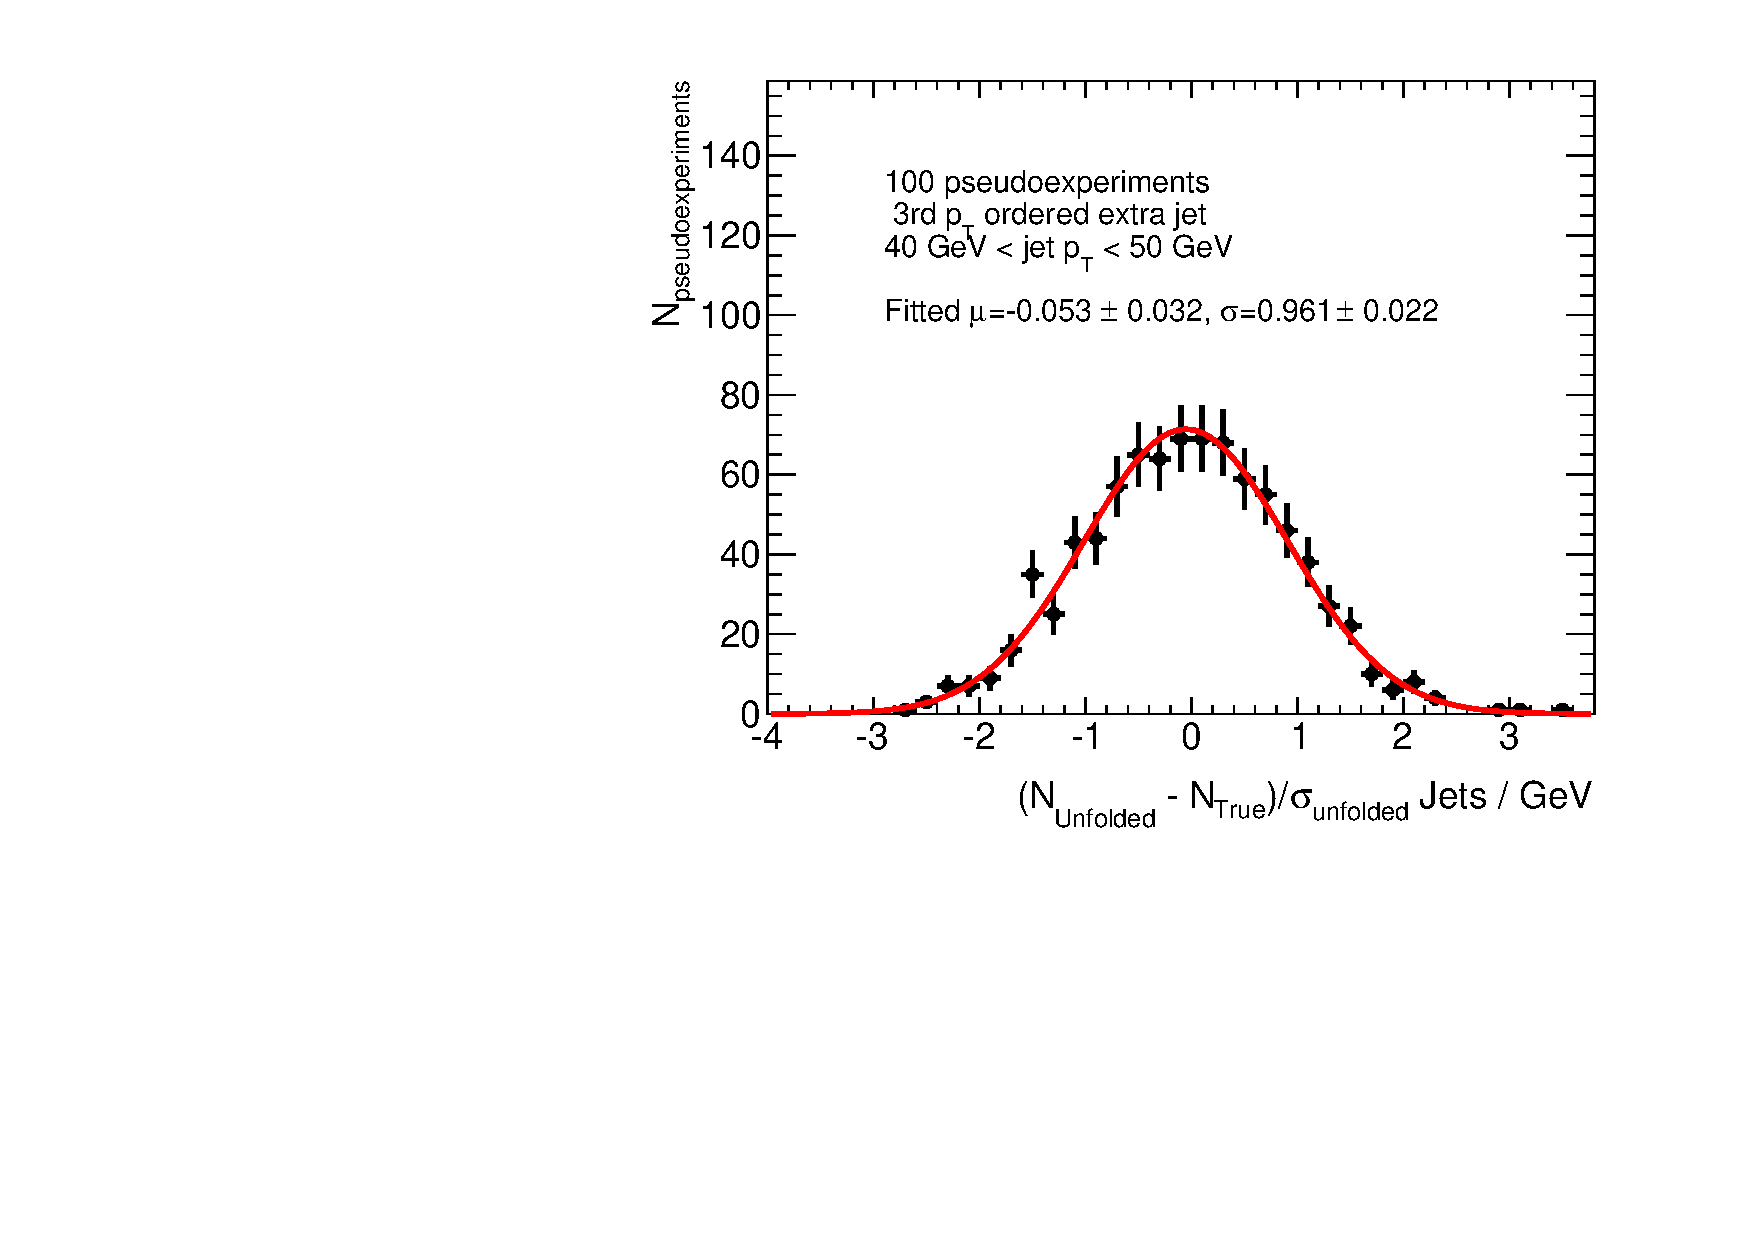
\includegraphics[width=0.33\textwidth]{fig/UnfoldPull/SingleSlicePull32.pdf}
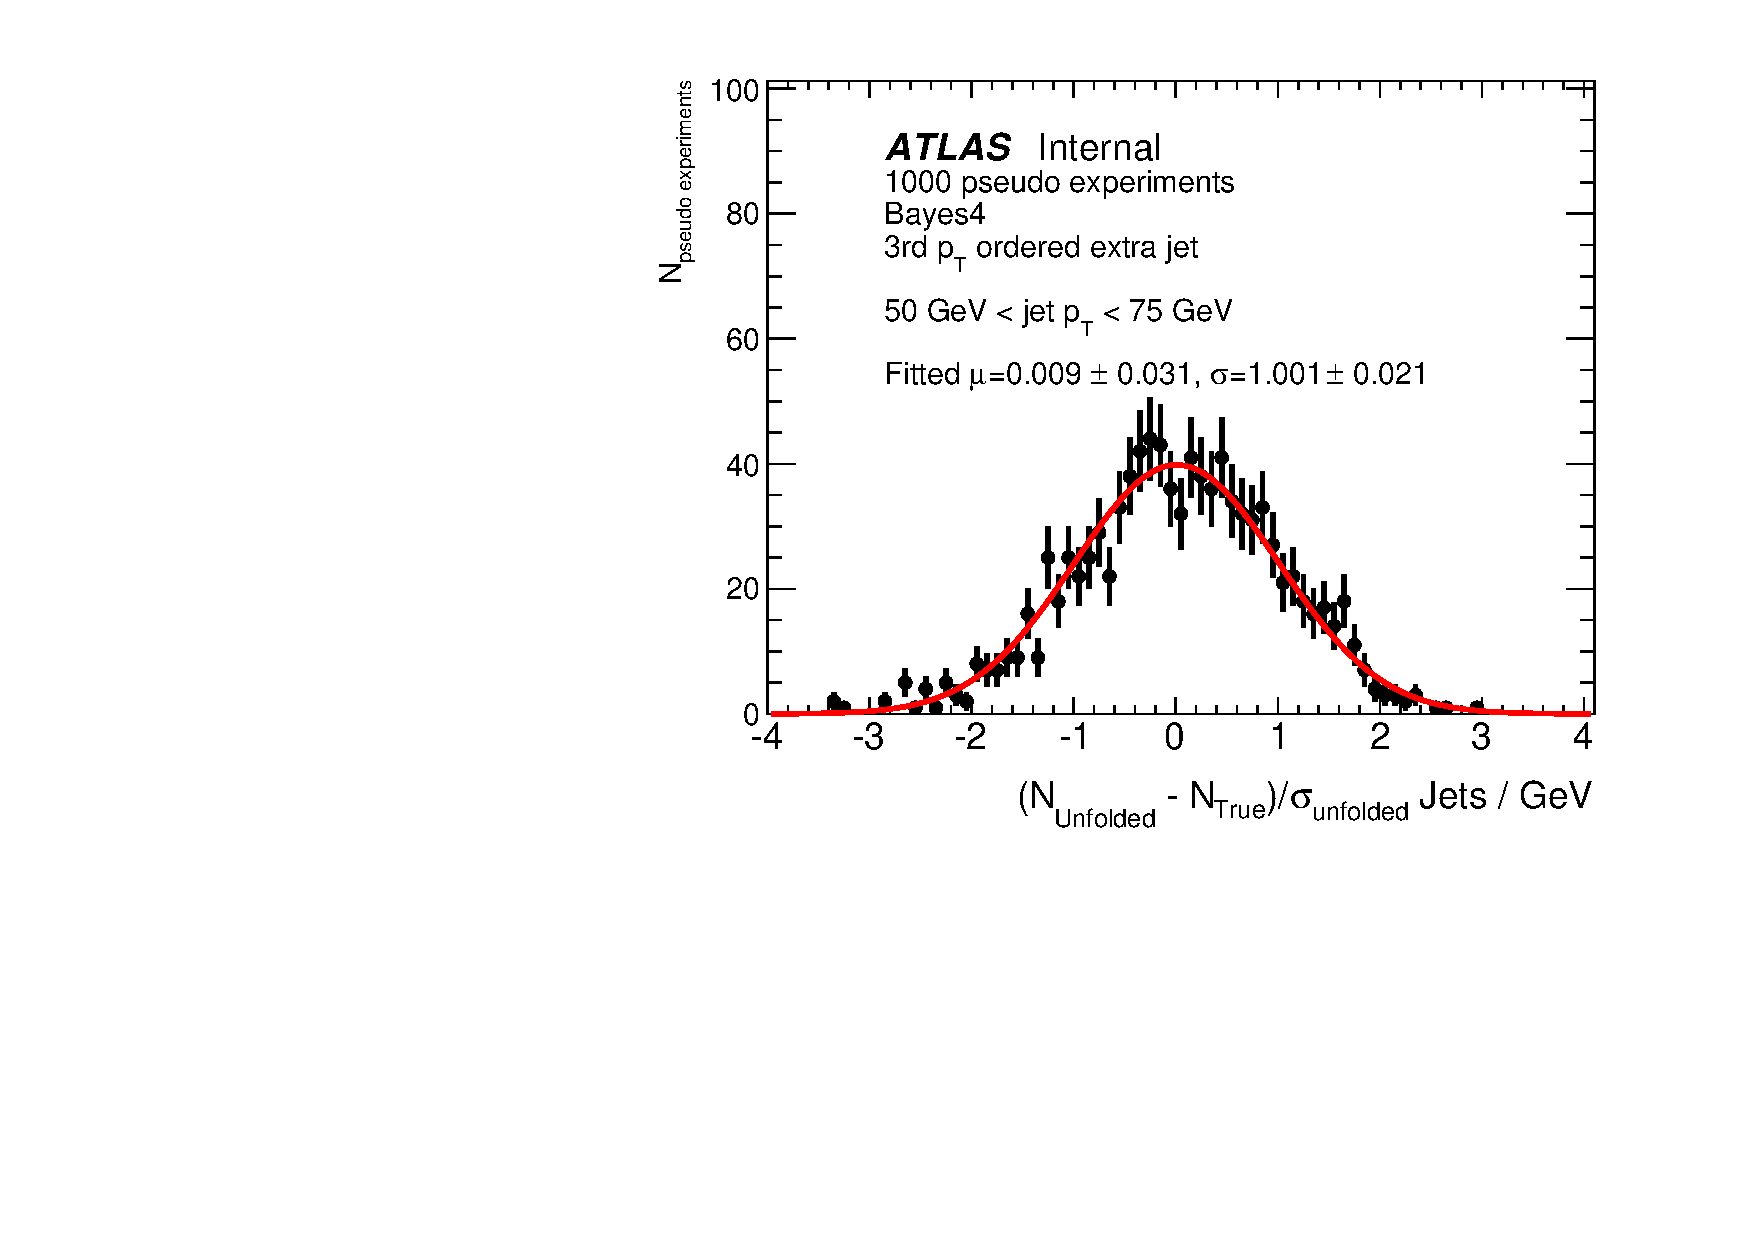
\includegraphics[width=0.33\textwidth]{fig/UnfoldPull/SingleSlicePull33.pdf}
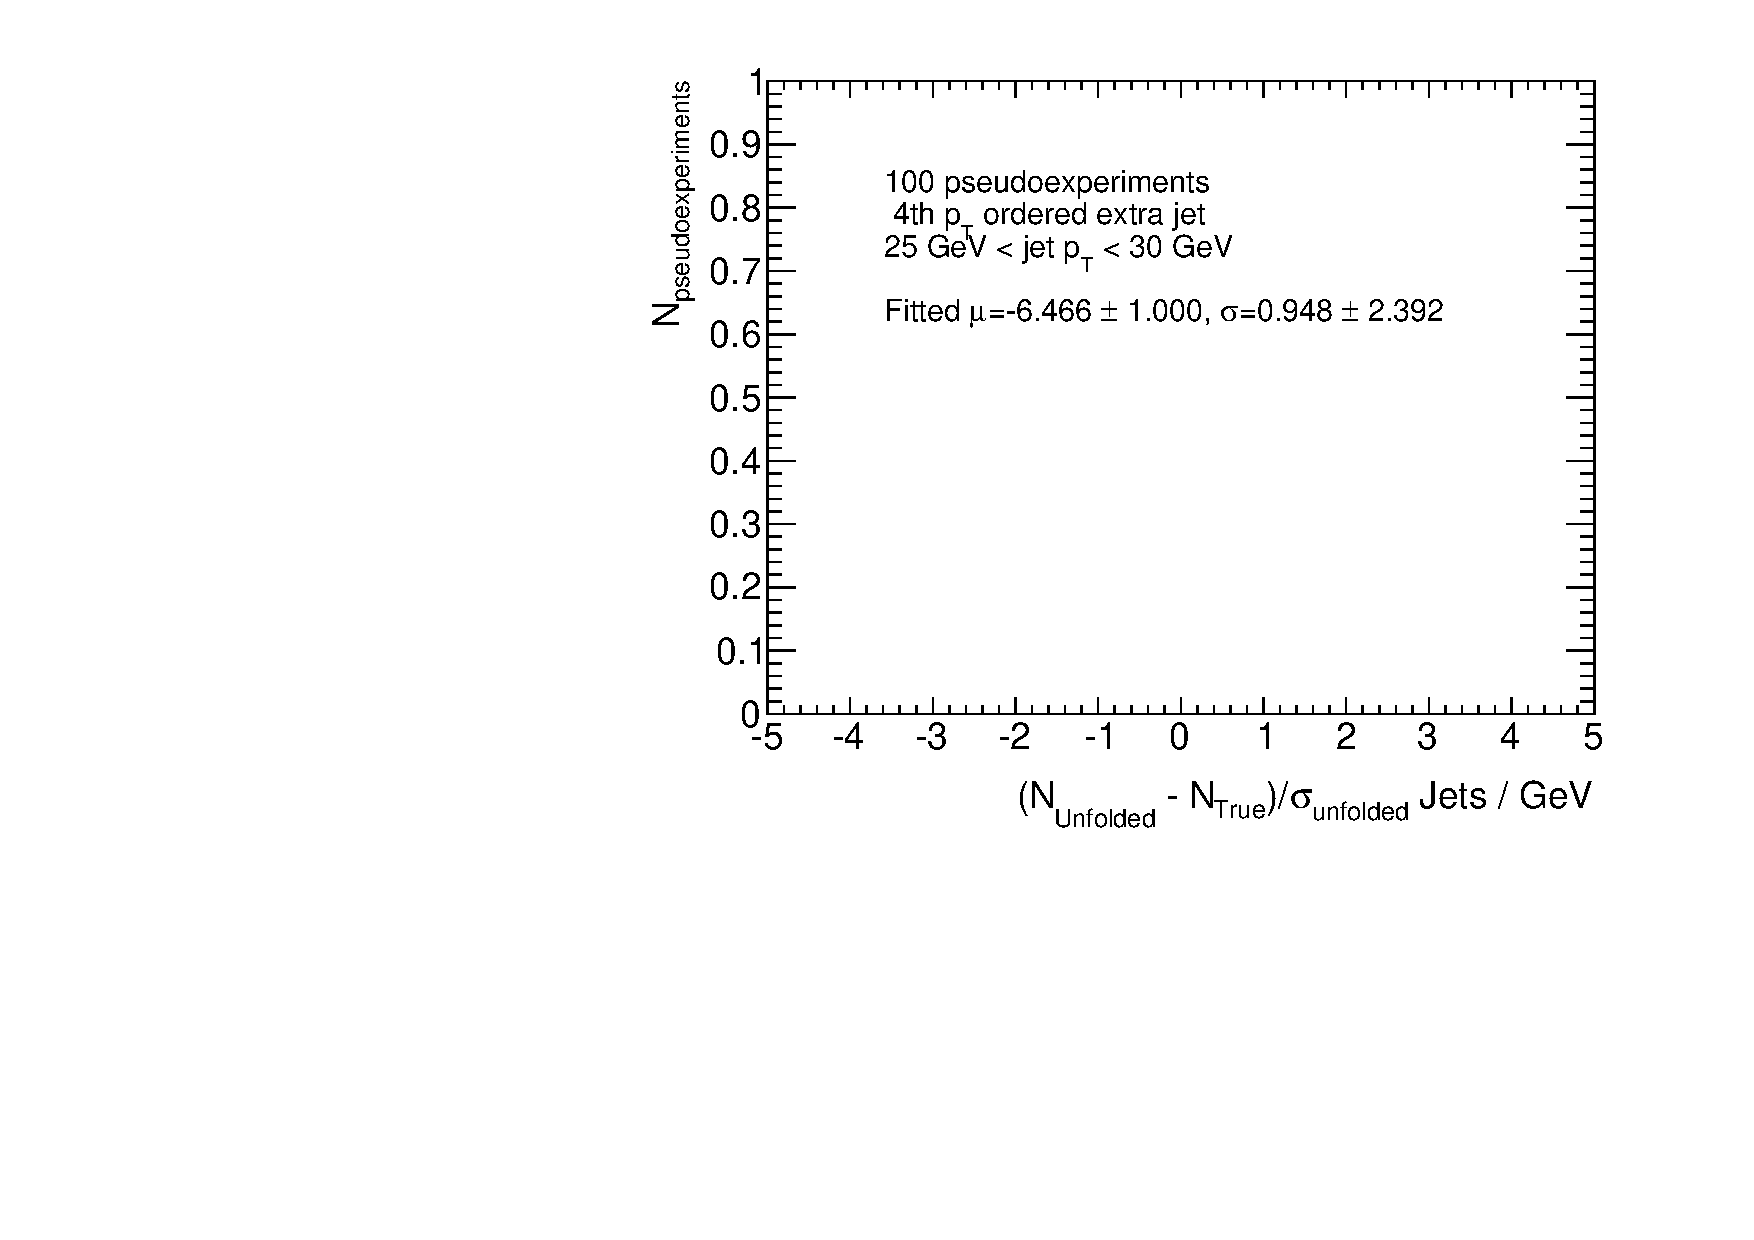
\includegraphics[width=0.33\textwidth]{fig/UnfoldPull/SingleSlicePull35.pdf}
%
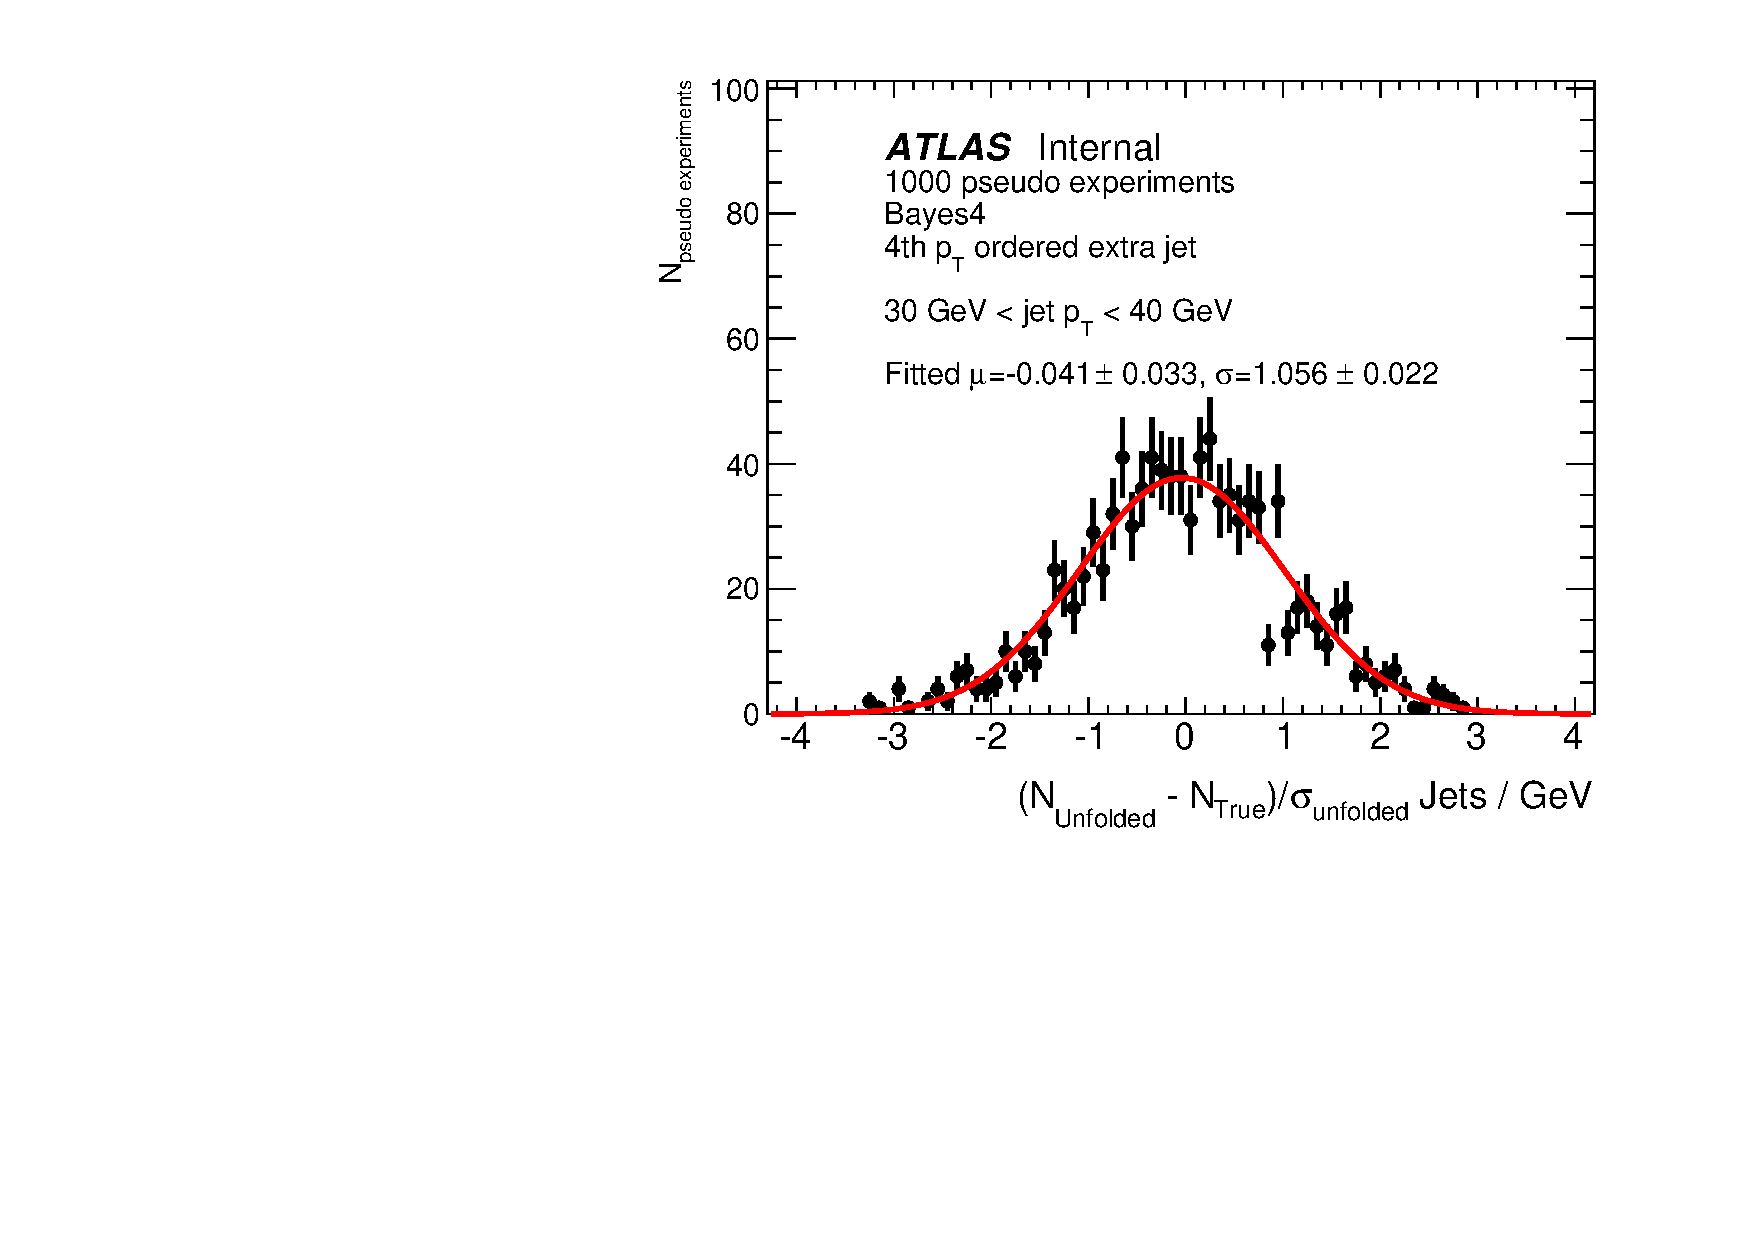
\includegraphics[width=0.33\textwidth]{fig/UnfoldPull/SingleSlicePull36.pdf}
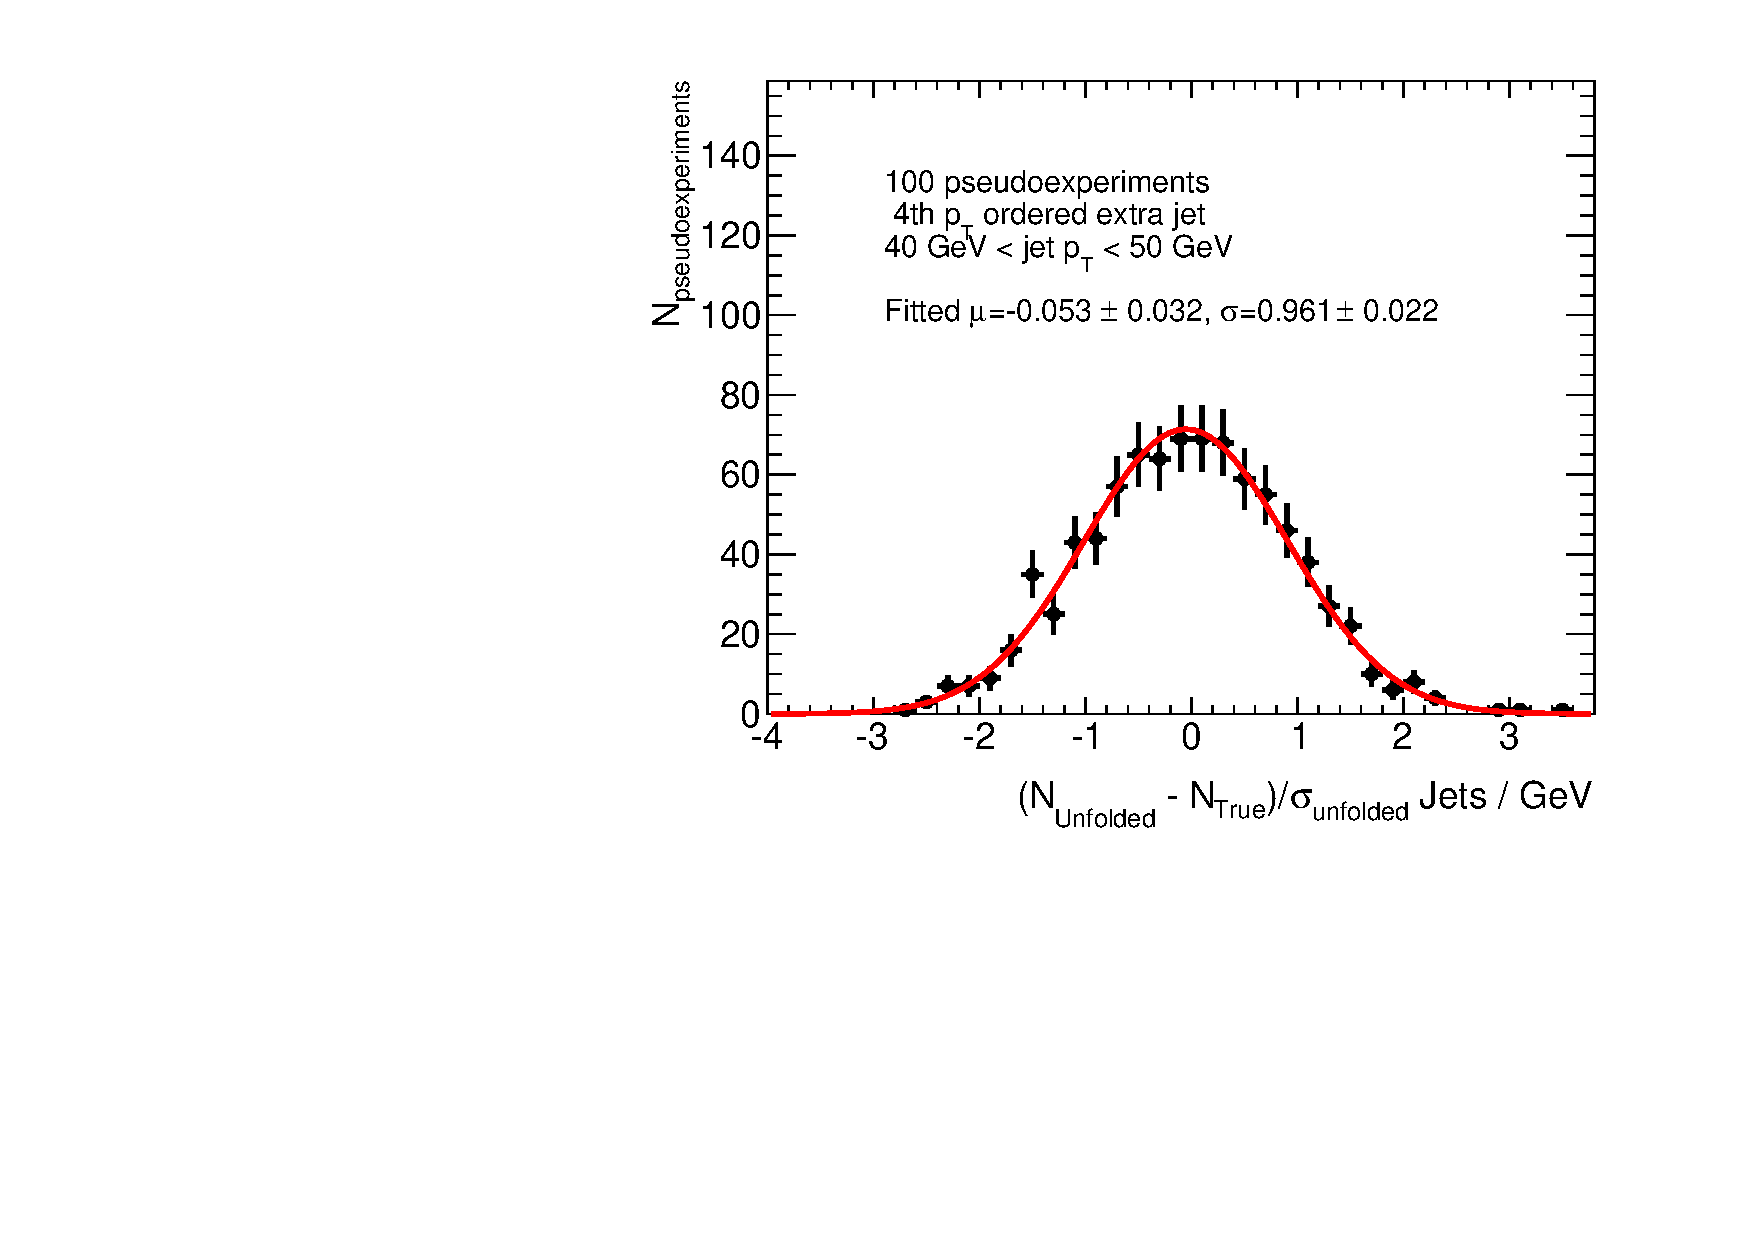
\includegraphics[width=0.33\textwidth]{fig/UnfoldPull/SingleSlicePull37.pdf}
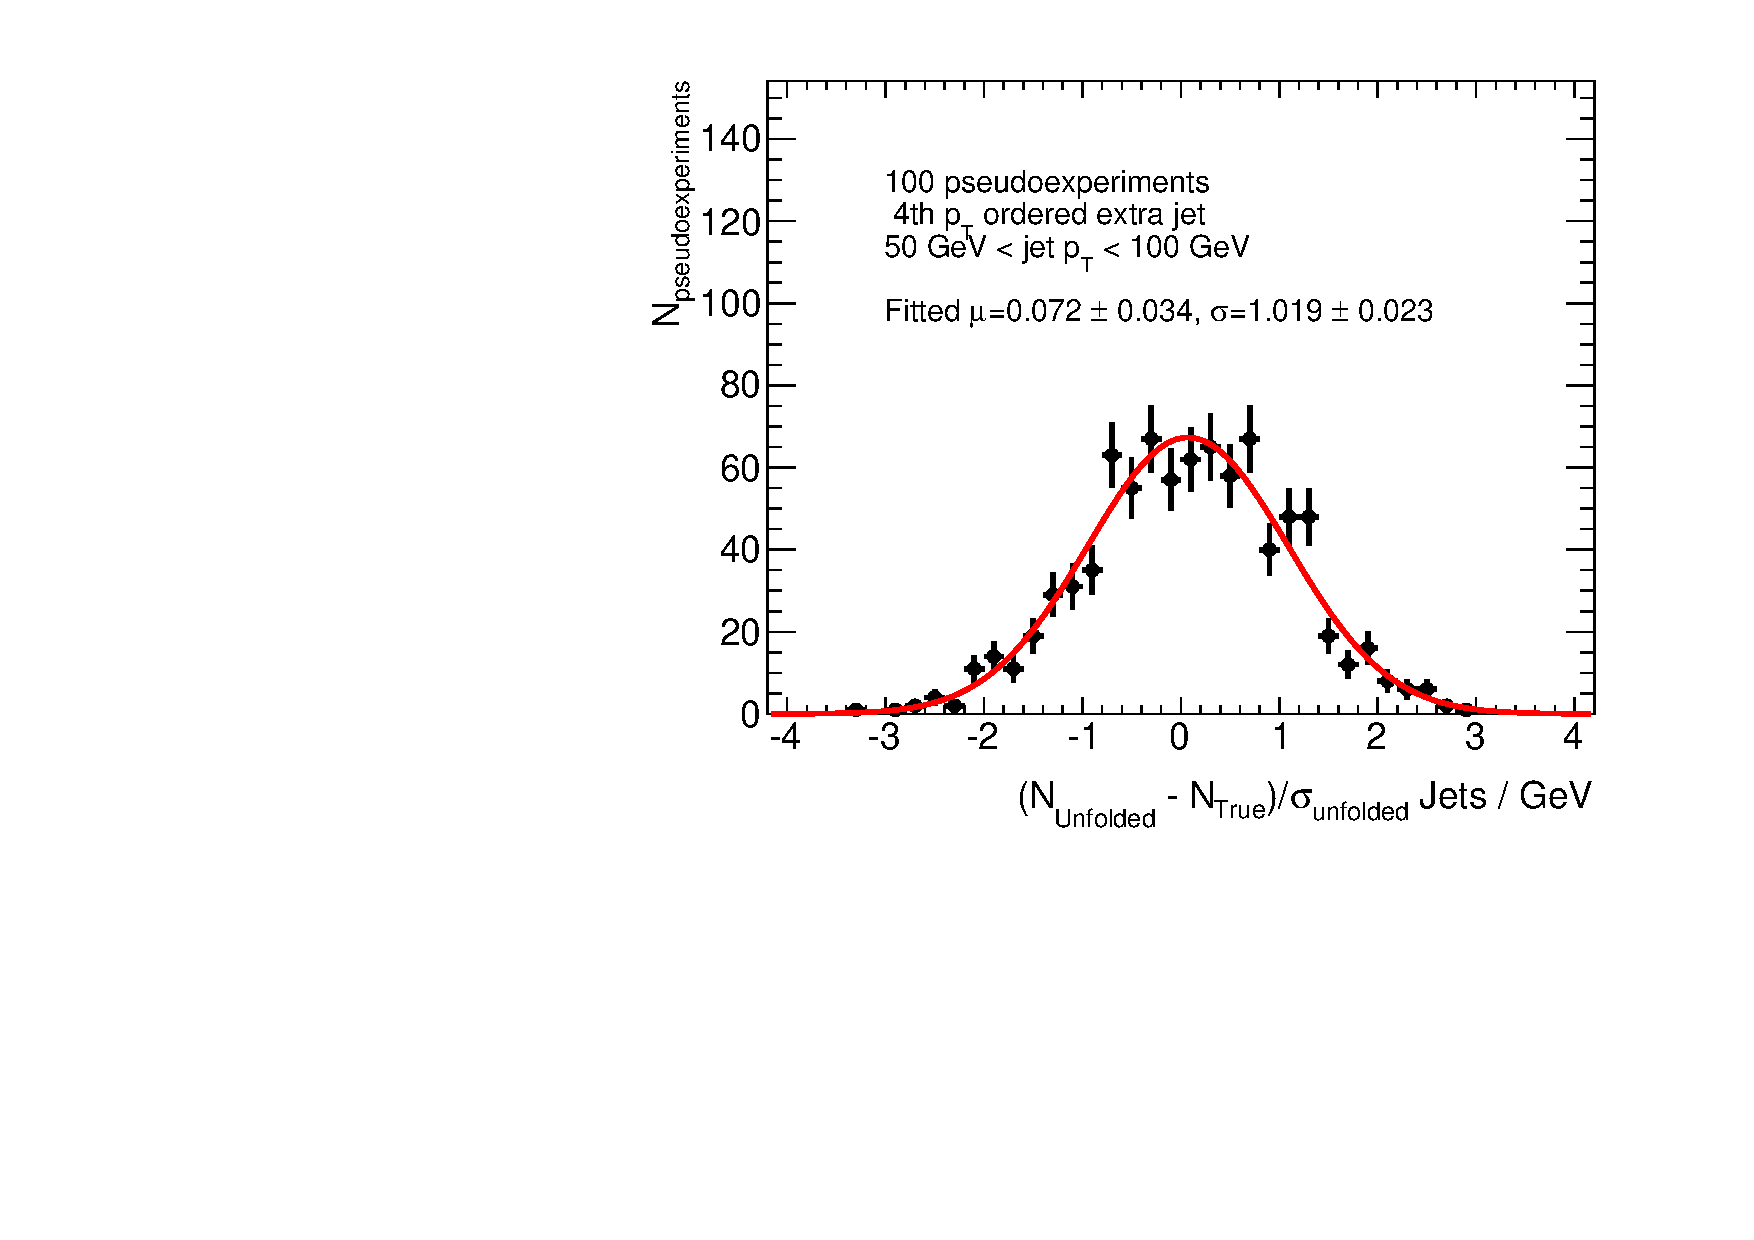
\includegraphics[width=0.33\textwidth]{fig/UnfoldPull/SingleSlicePull38.pdf}
%
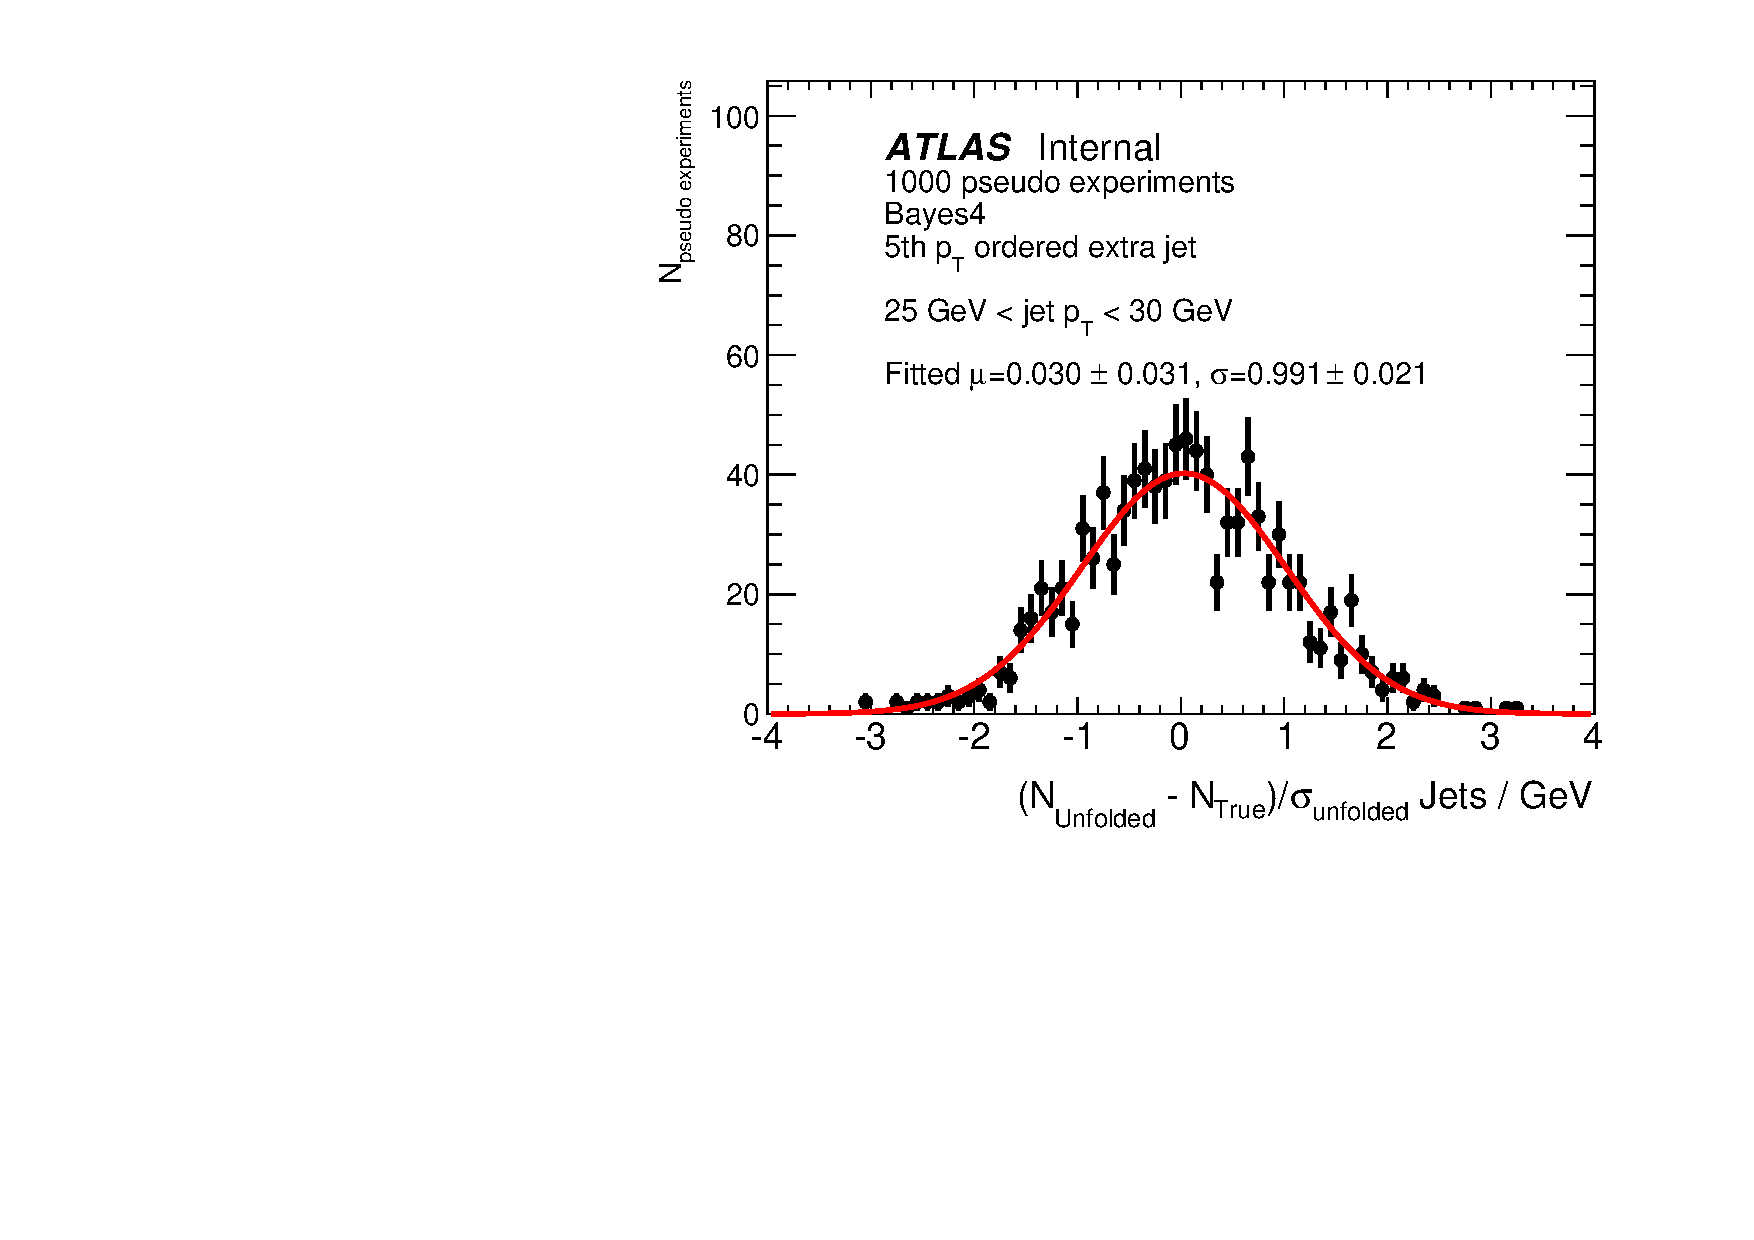
\includegraphics[width=0.33\textwidth]{fig/UnfoldPull/SingleSlicePull39.pdf}
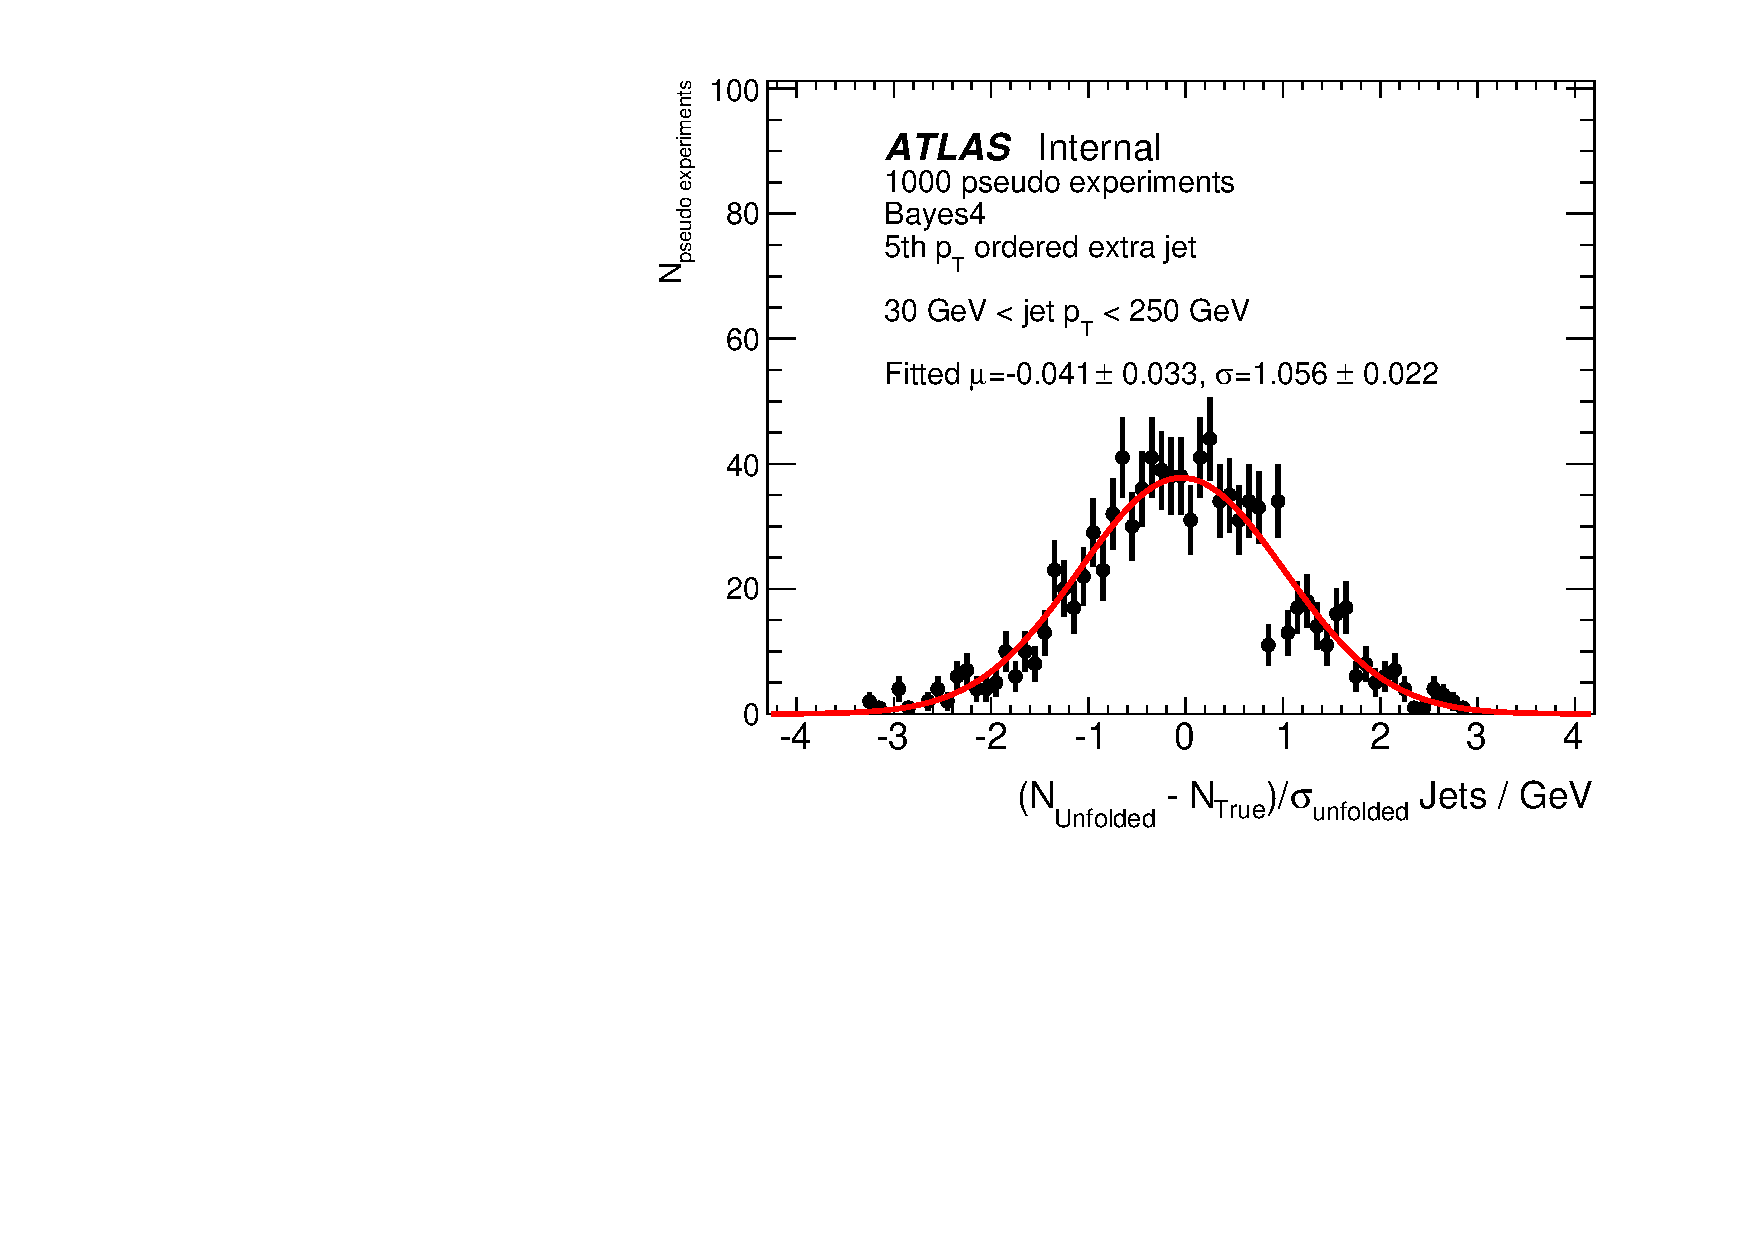
\includegraphics[width=0.33\textwidth]{fig/UnfoldPull/SingleSlicePull40.pdf}
%
\caption{Pull distributions for the extra jets from the baseline \ttbar\ +Wt simulation (\powpy) unfolded against a matrix filled with the baseline \ttbar\ +Wt simulation (\powpy). The Bayesian unfolding method 4 iterations is used. One thousand pseudoexperiments, each the size of the events in data, are randomly selected from the sample and unfolded.  A Gaussian is fit to the distributions of biases over the pseudoexperiments}
\label{fig:appPull2}
\end{figure}
\clearpage
